\documentclass[	
	12pt,								
	openany,               						
	oneside,			
	a4paper,
	abnt,						
	chapter=TITLE,						
	sumario=abnt-6027-2012,	 	
	english,										
	brazil												
]{faeterj-rio-abntex2}		



% --------------------------------------------------------------------
%
%            			INICIO DO DOCUMENTO 
%
% --------------------------------------------------------------------

\begin{document}
    % \citebrackets[]
    \citeoption{abnt-full-initials=yes}
    
    \pagestyle{empty}
	\selectlanguage{brazil}						%
	\frenchspacing								%
	\pretextual									%
	\imprimircapa								%
	\imprimirfolhaderosto*						%

    %\imprimirfichacatalografica
    %{666.555}  % esse número deve ser montado com a ajuda da biblioteca do IME
    %{S455h}
    %{Silva, F., Tal, C.} % <último nome>, <abreviação do primeiro nome>
    %{Projeto de Fim de Curso (PFC)}
    %{%
    %  1. Curso de engenharia da computação - Projeto Final de Curso.
    %  2. Um Assunto.
    %  3. Outro Assunto.
    %  I. Silva, Cilano.
    %  II. Beltrano, Fulano.
    %  III. \@title.
    %  IV. Instituto Militar de Engenharia.}
     %{Técnicas de blablabla}
	% --------------------------------------------------------------------
	% Insira abaixo os elementos prétextuais
	% 	como: folha de aprovação, dedicatória, agradecimentos, epigrafe,
	% 	resumo e listas de ilustrações, tabelas, siglas e simbolos.
	% --------------------------------------------------------------------
	
% Isto é um exemplo de Ficha Catalográfica, ou ``Dados internacionais de
% catalogação-na-publicação''. Você pode utilizar este modelo como referência.
% Porém, provavelmente a biblioteca da sua universidade lhe fornecerá um PDF
% com a ficha catalográfica definitiva após a defesa do trabalho. Quando estiver
% com o documento, salve-o como PDF no diretório do seu projeto e substitua todo
% o conteúdo de implementação deste arquivo pelo comando abaixo:
%
% \begin{fichacatalografica}
%     \includepdf{fig_ficha_catalografica.pdf}
% \end{fichacatalografica}

\begin{fichacatalografica}
	\sffamily
	\vspace*{\fill}					% Posição vertical
	\begin{center}					% Minipage Centralizado
	\fbox{\begin{minipage}[c][7,5cm]{12.5cm} 		% Largura
	\small
	
	C198m 
	\vspace{-0.3cm}
	\hspace{0.2cm}
	\parbox[t]{11cm}{
	%Sobrenome, Nome do autor
	Silva, Filipe Rodrigues Cardoso da
	
	\hspace{0.5cm} %\imprimirtitulo \imprimirautor. --
	%\imprimirlocal, \imprimirdata-
	Utilizando Coloração de Grafos de Interseção para Resolver o Problema de Programação de Horários de Exames em Universidades / Filipe Rodrigues Cardoso da Silva. – Rio de Janeiro: [s. n.], \imprimirdata.
	
	\hspace{0.5cm} \pageref{LastPage} p. 29 cm.\\
	
	\hspace{0.5cm}%  \imprimirorientadorRotulo~\imprimirorientador\\
	
	\hspace{0.5cm}
	%\parbox[t]{11.9cm}{
	Trabalho de Conclusão de Curso (Graduação em Tecnólogo
em Análise e Desenvolvimento de Sistemas) ~--~ Faculdade de Educação Tecnológica do Estado do Rio de Janeiro - FAETERJ-Rio, 
	\imprimirdata.
	%}
	\\
	
	\hspace{0.5cm}
	1. Coloração de Grafos. 
	2. Grafos de Interseção. 
	2. Programação de Horários de Exames em Universidades. 
	I. Silva, Filipe Rodrigues Cardoso da. 
	II. FAETERJ-Rio. 
	III. Utilizando Coloração de Grafos de Interseção para Resolver o Problema de Programação de Horários de Exames em Universidades  			
	}
	\begin{flushright}
	CDD 371.2
	\end{flushright}
	\end{minipage}}
	\end{center}
	
\end{fichacatalografica}
% ---
	% \include{TCC/capitulos/02.folha_de_aprovacao}
	
	% dedicatória
	
	% agradecimentos
	
	% epigrafe
	\begin{epigrafe}
    \vspace*{\fill}
	\begin{flushright}
		\textit{``Não diga pouco em muitas palavras,  \\
		mas sim muito em poucas. \\
		(PITÁGORAS)}
	\end{flushright}
\end{epigrafe}
% ---
	
	% resumo 
	 
% resumo em português
\setlength{\absparsep}{12pt} % ajusta o espaçamento dos parágrafos do resumo
\begin{resumo}

Ao agendar avaliações semestrais de uma universidade, pode-se identificar um clássico problema de combinatória, que vem sendo objeto de estudo na literatura desde a década de 1960. Este trabalho objetiva-se em apresentar o problema de programação de horários de exames universitários, suas características e restrições, bem como a modelagem matemática das turmas e alunos com a utilização de Grafos de Interseção. Será proposta uma heurística para aplicar o método de solução recorrendo à otimização de um problema de Coloração Generalizada de Grafos. Neste trabalho será apresentado um protótipo desenvolvido, e sua respectiva documentação, para permitir aos usuários a utilização do método de solução proposto de forma amigável.

 \textbf{Palavras-chave}: Problema de Programação de Horários de Exames em Universidades. Grafos de Interseção. Coloração de Grafos. Otimização.

\end{resumo}

% resumo em inglês
\begin{resumo}[Abstract]
 \begin{otherlanguage*}{english}
 
When scheduling semester examinations at a university, one can identify a classic combinatorial problem, which has been a study in the literature since the 1960s. This work aims to present the Examination Timetabling Problem, their characteristics and restrictions, as well as the mathematical modeling of classes with the use of Intersection Graphs. A heuristic will be proposed to apply the solution method using the optimization of a Generalized Graph Coloring Problem. In this work, will be presented a developed prototype and its respective documentation to allow users to use the proposed solution method in a friendly way.

   \vspace{\onelineskip}

\noindent
  \textbf{Keywords}:  Examination Timetabling Problem. Intersection Graphs. Graph Coloring. Optimization.
 \end{otherlanguage*}
\end{resumo}

% resumo em francês
%\begin{resumo}[Résumé]
% \begin{otherlanguage*}{french}
%    Il s'agit d'un résumé en français.

%   \textbf{Mots-clés}: latex. abntex. publication de textes.
% \end{otherlanguage*}
%\end{resumo}

% resumo em espanhol
%\begin{resumo}[Resumen]
% \begin{otherlanguage*}{spanish}
%   Este es el resumen en español.
%
%   \textbf{Palabras clave}: latex. abntex. publicación de textos.
% \end{otherlanguage*}
%\end{resumo}
% ---
	 
	% -----------------------------------------------
	%          Sumário (Não Altere)
	% -----------------------------------------------
	\pagestyle{simple}											%
    \stepcounter{tocdepth}	
    \pdfbookmark[0]{\listfigurename}{lof}
    \listoffigures*
    \cleardoublepage
    \pdfbookmark[0]{\listtablename}{lot}
    
    % Siglas
    \begin{siglas}
  \item[PPH] Problema de Programação de Horários
  \item[PPHE] Problemas Programação de Horários em Escolas 
  \item[PPHC] Problemas Programação de Horários de Cursos 
  \item[PPHEU] Problemas de Programação de Horários de Exames em Universidades
  \item[GGCP] \textit{Generalized Graph Coloring Problem}
  \item[LF] \textit{Largest-first}
  \item[HTML] \textit{Hypertext Markup Language}
  \item[CSS] \textit{Cascading Style Sheet}
  \item[PHP] \textit{PHP: “Hypertext Processor”}
  \item[RF] Requisito do Software
  \item[RN]  Regra de Negócio
  \item[UC] \textit{User Case} (Caso de Uso)
  \item[DER, ER] Diagrama de Entidade-Relacionamento
  \item[ICT] \textit{International Competition Timetabling}
 % \item[]
 % \item[]
 % \item[]
 % \item[]
\end{siglas}
% ---

\begin{simbolos}
  \item[$G$, $G(V, E)$] um grafo simples.
  \item[$V(G)$] conjunto de vértices de um grafo.
  \item[$v$, $w$] um vértice específico pertencente à $V(G)$.
  \item[$E(G)$] conjunto de arestas de um grafo.
  \item[$e$] uma aresta específica pertencente à $E(G)$.
  \item[$|V|$,  $n$] número de nós (vértices de um grafo).
  \item[$H(V, E)$] um multigrafo. 
  \item[$D(V, E)$] um grafo direcionado (digrafo).
  \item[$\mathbb{N}$] conjunto dos números naturais.
  \item[$p$] um rótulo de peso pertencente à \mathbb{N}.
  \item[$p(v, w)$, $p(e)$] um peso atribuído a uma aresta.
  \item[$\in$] simbolo matemático de pertence.
  \item[$k$] quantidade de horários disponíveis para realização das provas.
  \item[$K$] conjunto dos horários disponíveis para realização das provas $\in \mathbb{N}$.
  \item[$\chi(G)$] número cromático do grafo.
  \item[$C$] conjunto das possíveis colorações para o grafo.
  \item[$c$] uma coloração para o grafo.
  \item[$P_c$] quantidade de provas de segunda chamada necessárias para uma coloração $c$.
 % \item[]
 % \item[]
 % \item[]
 % \item[]
 % \item[]
 % \item[]
 % \item[]
\end{simbolos}
    % Símbolos
    
    \listoftables*
    \cleardoublepage
 	\pdfbookmark[0]{\contentsname}{toc}
    \tableofcontents*
    \cleardoublepage								%
 	%\settocdepth{section}						%
 	\cleardoublepage
	% ------------------------------------------------
	%               Fim do Sumário
	% ------------------------------------------------

	\textual									%
	% --------------------------------------------------------------------
	% Insira abaixo os capitulos da sua parte textual 
	% como: Introdução e os capitulos referentes ao desenvolvimento do trabalho
	% --------------------------------------------------------------------
	
	\chapter*[Introdução]{Introdução}
\setcounter{chapter}{1}
\addcontentsline{toc}{chapter}{INTRODUÇÃO}
\pagestyle{simple}
% ----------------------------------------------------------


% \section{Apresentação Geral}

Os problemas de programação de horários vem sendo estudados desde o início da década de 60, são problemas cotidianos e muitas vezes de difícil resolução. A dificuldade surge devido à natureza combinatória do problema, o que demanda grande esforço e tempo para se solucionar manualmente em alguns casos. Para isso é comum se propor soluções computacionais que sejam capazes de buscar a melhor programação dos horários no menor tempo e com menor esforço possível.

Para permitir a utilização de computadores na resolução de um problema cotidiano, precisaremos realizar um processo de modelagem na qual transformaremos o problema real em um problema de computador, e a partir desse momento utilizaremos os algoritmos, possibilitando que o computador execute uma série de instruções específicas de forma sequencial. 

Este trabalho apresentará o processo de modelagem e confecção de um protótipo de sistema para solucionar um clássico problema de natureza combinatória, observado em universidades.

% \section{Problema Geral}
Apresentaremos ao longo deste trabalho uma proposta de resolução para o \textbf{Problema de Programação de Horários de Exames em Universidades} (PPHEU), nomeado por \citeonline{schaerf99} e se caracteriza por ser de difícil resolução manual e bastante estudado por pesquisadores da área.

A aplicação de exames, provas ou avaliações em universidades, se torna um problema de natureza combinatória em algumas circunstâncias, e caso isso venha a ocorrer, encontrar uma solução perfeita pode ficar até mesmo impossível em alguns cenários. Nesses casos é recomendável a busca da melhor solução possível, maximizando (ou minimizando) determinado aspecto dela visando encontrar uma solução ótima através dessa otimização.

Os problemas de programação de horários de exames universitários foram vastamente estudados em trabalhos como os de \citeonline{kiaer92}, \citeonline{socha03}, \citeonline{lai08}, \citeonline{burke10} entre outros, onde são utilizadas diversas formas de modelagem e métodos de solução, contudo foram os trabalhos de \citeonline{brown87}, \citeonline{vredeveld_02} e \citeonline{scheeren18} que utilizaram as formas de modelagem ou solução mais similares as apresentadas neste trabalho.

% \section{Problema Específico}

A \textbf{programação de horários de exames universitários}, consiste na criação de uma tabela de horários para que diversas turmas de uma universidade realizem suas provas semestrais. Contudo, condições adicionais podem ser destacadas, por afetarem consideravelmente a solução e por consequência o resultado obtido.

Inicialmente, deve-se compreender turma em um contexto universitário, isto é, uma turma está diretamente relacionada a uma única disciplina ofertada semestralmente, e que seus alunos podem ou não integrarem ela, de acordo com o interesse do aluno e das normas da instituição. Com isso, temos um ambiente onde duas turmas podem ou não ter alunos em comum.

Ao estipularmos o horário em que uma turma deverá realizar uma prova, deveremos considerar que se duas, ou mais, turmas com alunos em comum realizarem seus exames de forma simultânea, os alunos terão avaliações em diferentes turmas no mesmo horário, com isso serão prejudicados e deverão realizar a segunda chamada dos exames que não puderam fazer em decorrência da alocação dos horários.

Caso uma instituição possua uma quantidade limitada de horários para a realização das provas, poderá não ser possível realizar a programação dos exames de forma a nenhum aluno ser prejudicado por conflitos nos horários de prova, assim buscaremos minimizar o número de provas de segunda chamada necessárias.


% \section{Objetivos Gerais}

Este trabalho trará uma abordagem em que se obtém o melhor resultado possível considerando as turmas, seus alunos e a quantidade de horários de provas disponíveis na instituição. Será apresentado conceitualmente e de forma prática na aplicação proposta, a melhor alocação e suas possíveis consequências, permitindo dessa forma, que sejam realizadas as aplicações das provas de segunda chamada.



% \section{Objetivos Específicos}



% Mesmo possuindo grande base conceitual e propostas de algoritmos que solucionam o problema, não foi proposto em nenhum desses trabalhos uma solução para um usuário final, considerando a utilização da solução por um leigo na parte matemática e algorítmica.


O objetivo deste trabalho é apresentar formalmente o problema de programação de horários de exames universitários com suas respectivas classificações e restrições, demonstrar a modelagem matemática para o problema e propor um algoritmo capaz de obter a melhor solução, além de apresentar um sistema que permita a busca pela resolução de forma automática e que seja amigável para qualquer usuário.

A \textbf{modelagem do problema} utilizará das estruturas matemáticas da \textbf{Teoria dos Grafos}, mais especificamente de \textbf{Grafos de Interseção} e \textbf{Coloração de Vértices}. Este modelo nos beneficiará com um enorme acervo de pesquisas, assim como observado em \citeonline{carlson66}, \citeonline{bondy78}, \citeonline{brown96}, \citeonline{kann97} e \citeonline{leung04}, que ajudam a facilitar a abordagem sobre tema, além de nos proporcionar uma adequação simplificada do modelo conceitual em um protótipo funcional.

Com o desenvolvimento de uma solução computacional, poderemos automatizar o processo de busca por soluções, permitindo obter uma solução com uma expressiva redução no tempo de busca em comparação com métodos manuais. 

O problema de programação de horários de exames universitários, pertence à família de problemas bem conhecidos  na computação e matemática, os \textbf{problemas de tabela de horários} (também conhecidos como \emph{Timetabling} ou \emph{Timetable}). 

Existem alguns exemplos de implementações amigáveis para o usuário final (\emph{user-friendly}), voltadas para o \emph{Timetabling} como, por exemplo, o “\textbf{Cronos}”\ de \citeonline{cronos20}, o “\textbf{GridClass}”\ de \citeonline{gridclass20} e o “\textbf{Urânia}”\ de \citeonline{urania20} sendo todos estes voltados para o problema de programação de horários escolares, onde, de forma simplificada, busca-se alocar professores e alunos em salas, em horários específicos, para a realização das aulas.

% \section{Metodologia / Estratégia}

% A documentação do processo, partindo da identificação de um problema de natureza combinatória até o desenvolvimento de um produto amigável para um usuário final, por meio da utilização de abstrações, estruturas e modelos matemáticos, não é comum em trabalhos de conclusão da instituição, contudo, visando uma maior disseminação dessas informações no âmbito da instituição e possibilitar a (re)utilização futura de partes deste trabalho em outros problemas de natureza similar decidimos seguir por este caminho.

% \section{Organização do Trabalho}

% Para desenvolver um “software” seja capaz de resolver o problema, mantendo sua simplicidade e sendo intuitivo ao máximo para os usuários finais, o problema deve estar bem estruturado, para que a solução encontrada por meio da aplicação seja satisfatória tanto do ponto de vista do usuário, quanto do ponto de vista conceitual. Com isso, iniciaremos a partir da análise do problema cotidiano, por consequência o problema do usuário, a quem se destinará a aplicação.

Este trabalho está organizado da seguinte forma.

No capítulo \ref{cap:problema} são apresentados os \textbf{Problemas de Escalonamento de Horários}, sua origem e suas subdivisões, incluindo a que pertence o problema de programação de horários de exames universitários.

No capítulo \ref{cap:modelagem} é demonstrada a \textbf{Modelagem Matemática}, apresentando fundamentos sobre Teoria dos Grafos e a forma pela qual os grafos de interseção foram utilizados.

No capítulo \ref{cap:solucao} é apresentado o \textbf{Método de Solução} que explica a forma pela qual utilizamos a modelagem apresentada no capítulo anterior para resolver o problema e os algoritmos propostos para isso.

No capítulo \ref{cap:software} está a \textbf{Documentação UML} relativa à aplicação desenvolvida, com as tecnologias usadas, metodologias e especificações do “software”.

No capitulo \ref{cap:resultados} estão descritos os \textbf{Resultados Obtidos} com o desenvolvimento do trabalho e são apresentadas as motivações e objetivos para os \textbf{Trabalhos Futuros}.

Por fim é apresentada no capítulo \ref{cap:conclusao} as \textbf{Considerações Finais} acerca do trabalho desenvolvido, as \textbf{Limitações de Pesquisa} observadas ao decorrer do trabalho e as \textbf{Recomendações para Pesquisas Futuras}, onde são apresentadas as recomendações para futuros estudos e trabalhos de motivação similar ao apresentado.

Em apêndice \ref{cap:roteiro} está descrito o roteiro para realização de um teste de usabilidade do sistema proposto, onde busca-se observar se os objetivos do desenvolvimento foram atingidos juntamente a usuários reais.

No anexo \ref{cap:manual} está o \textbf{Manual} para instalação e utilização do protótipo criado com base nas especificações do capítulo \ref{cap:software}, enquanto o anexo \ref{cap:resultado} apresenta um exemplo do \textbf{Relatório} sobre o resultado emitido pelo protótipo ao final da resolução do problema.


	
	%\part{Proposta de Desenvolvimento e Metodologia}
 	\phantompart
 	
 	\chapter{Problemas de Escalonamento de Horários}
\pagestyle{simple}
\label{cap:problema}

% ---
%
% ---
% A descrição do problema será voltada para o leitor leigo no assunto, onde será apresentado o problema, e o objetivo de se realizar um estudo sobre esse problema e qual a finalidade do mesmo.
%
% Versão atual da descrição: 2018/12/26 - 1.1.0 - Não revisada
% ----
% Problema de Agendamento (Scheduling)
Problemas de escalonamento de horários (\textit{scheduling}), são problemas amplamente estudados na matemática e computação, são tidos como problemas clássicos de otimização combinatória. Resumidamente, \citeonline{wren96} define esses problemas como: agendar recursos em horários, respeitando condições prévias, de forma a minimizar o custo total de algum conjunto de recursos utilizados. 

O problema de escalonamento é vastamente explorado na literatura por ser aplicável a muitas situações que envolvam alocar um ou mais recursos (como pessoas, veículos, maquinário, processadores e etc) em um quadro limitado de horários, onde se deseja maximizar (ou minimizar) alguma característica da solução que esteja em função de algum recurso, sem violar as regras inerentes ao problema enunciado. Na literatura muitas classes de sub-problemas de escalonamento são apresentados, dentre essas, uma que se destaca é o Problema de Programação de Horários (PPH), também chamado de \textit{timetabling}.


\section{Timetabling}

% Apresentar o Timetabling
O PPH foi primeiramente apresentado por \citeonline{gotlieb63}, demonstrando o problema de alocar professores, turmas e salas em determinados horários de aula, de forma a não se ter um mesmo professor em duas salas em um mesmo horário ou dois professores em uma mesma sala simultaneamente. 

O PPH é definido por \citeonline{wren96} como sendo a atribuição, sujeita a restrições, de recursos a eventos dispostos em quantidade de espaço e tempo limitados, visando satisfazer da melhor forma um conjunto de objetivos estabelecidos. Contudo, essa atribuição pode vir a possuir um alto grau de complexidade de acordo com as restrições e os objetivos a serem atingidos. 

% Tipos de Timetabling
Existe um grande volume de informações referentes ao PPH, sendo apresentadas formas de solução, aplicação e classificação. Em \citeonline{rocha13} os problemas de PPH são classificados de acordo com suas aplicações, podendo ser: Escalas de Trabalhadores (\textit{Employee Timetabling}), Escalas de Condutores de Veículos de Transporte (\textit{Transportation Timetabling}), Escalas de Jogos de Competições Esportivas (\textit{Sports Timetabling}), Educacional (\textit{Educational Timetabling}).


\subsection{Problemas de Programação de Horários Educacionais (\textit{Educational Timetabling})}

% Apresentar os Educacionais
Os PPH Educacionais são os problemas cujas características (restrições e recursos) são semelhantes a situações enfrentadas em instituições de ensino, como em definir o quadro de aulas, calendário de provas universitárias, distribuição de turmas em salas de aula entre outros. Segundo \citeonline{santos07}, os PPH da área educacional podem ser especificados em três categorias: Problemas Programação de Horários em Escolas (PPHE),  Problemas Programação de Horários de Cursos (PPHC) e Problemas de Programação de Horários de Exames em Universidades (PPHEU). 

Em \citeonline{schaerf99} pode ser observada a seguinte classificação:

\begin{itemize}
\item PPHE: A programação semanal para todas as classes de uma escola, evitando que os professores possuam duas aulas ao mesmo tempo, e vice-versa;
\item PPHC: A programação semanal de todas as palestras de um conjunto de disciplinas universitárias, minimizando as sobreposições de palestras de disciplinas que possuem alunos comuns;
\item PPHEU: O agendamento para os exames de um conjunto de disciplinas universitárias, evitando a sobreposição de exames de cursos com alunos comuns, e evitando, o melhor possível, que os alunos tenham exames muito próximos.
\end{itemize}


% Classificação do problema
Os PPH Educacionais estão entre os problemas mais difíceis da área de otimização combinatória. Podendo ainda serem aplicadas inúmeras novas restrições a problemas já enunciados, de modo a tornar o resultado obtido o mais próximo do ideal e/ou do mundo real, entretanto a dificuldade de se encontrar a melhor solução possível aumenta.

Em \citeonline{schaerf99} é visto que os PPH Educacionais são classificados como NP-Completo para a maioria das formulações. Dessa forma, a solução exata em curto tempo de execução só pode ser garantida para instâncias pequenas, que muitas vezes podem não corresponder à realidade da maioria das instituições de ensino.

\section{Problema de Programação de Horários de Exames em Universidades}
\label{subsec:desc_prob}
% !!! Descrever o problema
O problema consiste em definir horários de provas para diferentes turmas universitárias. Sendo uma turma universitária relacionada a apenas uma disciplina, diferente do contexto escolar, em que uma turma tem diversas disciplinas.

% !!! Descrever as restrições
Um mesmo aluno pode pertencer a diferentes turmas, dessa forma para que ele possa realizar suas provas, busca-se evitar a atribuição em um mesmo horário de diferentes avaliações para um mesmo aluno. Caso não seja possível criar uma grade de horários sem prejudicar nenhum aluno, sendo permitida a realização de avaliações de segunda chamada para aqueles que possuírem duas ou mais provas em um mesmo horário. 

Com isso deseja-se alocar as provas em horários buscando o menor número de avaliações de segunda chamada possível.

Neste trabalho iremos considerar esse problema como um problema de programação de horários de cursos universitários (PPHC). Que \citeonline{schaerf99} define como um problema semelhante ao de definir horários de exames (PPHEU), contudo, ele adverte que em situações onde as turmas são heterogêneas, o comum é definir o problema como um PPHC, onde os cursos (ou palestras) serão tratados como horários de avaliações.

\section{Criação de Horários de Exames em Universidades}

Uma solução trivial para o problema consistiria em ter um número de horários para realização da prova maior ou igual à quantidade de turmas. Com isso bastaria atribuir cada turma a um horário e não haveria nenhuma sobreposição e por consequência nenhuma prova de segunda chamada.
%% Inserir imagem apresentação
%%      --- Solução Trivial

Contudo, este trabalho focará em explorar as situações onde uma solução trivial não possa ser adotada. Isto é, quando a quantidade de turmas for maior que o número de horários disponíveis.

%% Inserir imagem apresentação
%%      --- Solução Não Trivial

Nesse cenário algumas turmas terão que, obrigatoriamente, compartilharem o mesmo horário de prova. Dessa forma, caso duas turmas possuam alunos em comum, a aplicação da prova de segunda chamada seria necessária para os alunos prejudicados.

Com isso o trabalho irá explorar como identificar as turmas com alunos em comum, de modo a minimizar a alocação em um mesmo horário dessas turmas. Dessa maneira minimizar a quantidade de provas de segunda chamada.





\section{Variações do problema}

No decorrer da pesquisa para realização deste trabalho, alguns problemas foram analisados (e consequentemente modelados) e pôde-se notar uma similaridade entre suas características.

Acreditamos que existam outros problemas que tenham características similares à estes apresentados, com isso a proposta de solução algorítmica (apresentada no \textbf{capitulo \ref{cap:solucao}}), visará resolve-los independente da descrição, obtendo resultados com a mesma qualidade.



\subsection{Alocação de Bandas em dias de um festival}
% !!! Descrever o problema
Um evento de música popular visa reunir diversos artistas, músicos independentes e amadores para se apresentar em diferentes palcos e horários. 

% !!! Descrever as restrições
Muitas bandas possuem membros em comum (definidos aqui como: um conjunto de pessoas que integrem a parte artística uma apresentação, seja instrumentista, dançarino, um técnico ou outros). Deseja-se evitar que muitas bandas sejam prejudicadas com a alocação de seus membros em diferentes palcos em um mesmo horário, pois, isso causaria um desfalque em uma das bandas.

Caso não seja possível evitar todos os desfalques, deve-se minimizar eles para que o festival ocorra do melhor modo possível.

\subsection{Escalas de Equipes em uma Companhia Aérea}
% !!! Descrever o problema
Uma companhia aérea separa seus comissários em diferentes equipes, podendo um comissário de voo estar em mais de uma equipe, a empresa deseja organizar os grupos a trabalhar em seus voos de forma que as equipes possam trabalhar com a menor quantidade de desfalques possível.

% !!! Descrever as restrições
Caso um comissário faça parte de uma ou mais equipes escaladas em um mesmo dia, esse desfalcará as demais equipes, pois, só poderá estar em um único voo, e um substituto deverá ser contratado para completar o grupo.

Deseja-se distribuir as equipes em diferentes voos buscando-se minimizar a quantidade de desfalques, e por consequência, contratações de substituintes.

\subsection{Distribuição de Recursos Militares}
% !!! Descrever o problema
Em uma operação militar existem diversos recursos, como equipamentos, armamentos, munições e especialistas, que devem ser distribuídos de melhor forma possível visando garantir o sucesso da missão.

% !!! Descrever as restrições
Ao se distribuir soldados em operações em diferentes lugares, busca-se formar separar as unidades militares de forma que subunidades sejam capazes de atuar de forma simultânea. Um soldado dessa forma é preparado para poder atuar em diferentes grupos caso seja necessário.

Quando diferentes operações demandam o destacamento das subunidades o oficial deve designar os soldados de forma a manter os grupos o mais coesos e similares aos grupos com os quais os soldados já realizaram treinamento.

Dessa maneira, um soldado de uma unidade pode pertencer a qualquer uma das subunidades com a qual já realizou treinamento, e caso seja designado a realizar uma operação com esse grupo, irá desfalcar os demais.

Deseja-se buscar uma distribuição das subunidades de forma que ocorra o menor número possível de desfalques nas operações. Visando concluir da melhor forma a missão recebida.

    
    %\include{capitulos/modelagem} 
    %definições de como foi modelado matematicamente o problema
    
 	\chapter{Modelagem Matemática}
\pagestyle{simple}
\label{cap:modelagem}

Visando permitir o uso do poder computacional na busca de uma solução para o problema apresentado no capítulo \ref{cap:problema}, necessita-se modelar o problema de forma matemática.

Dessa forma foi optado o uso da teoria dos grafos como estrutura matemática visando modelar o problema.

\section{Conceitos Gerais em Teorias dos Grafos}

Um grafo simples $G(V,E)$ é definido por \citeonline{szwarcifter86} como sendo uma estrutura matemática composta por um conjunto finito não vazio de vértices $V$ e um conjunto $E$ de pares, não ordenados, de diferentes vértices denominados arestas.

%% inserir imagem
%%  --- Grafo
\begin{figure}[H]
     \centering
     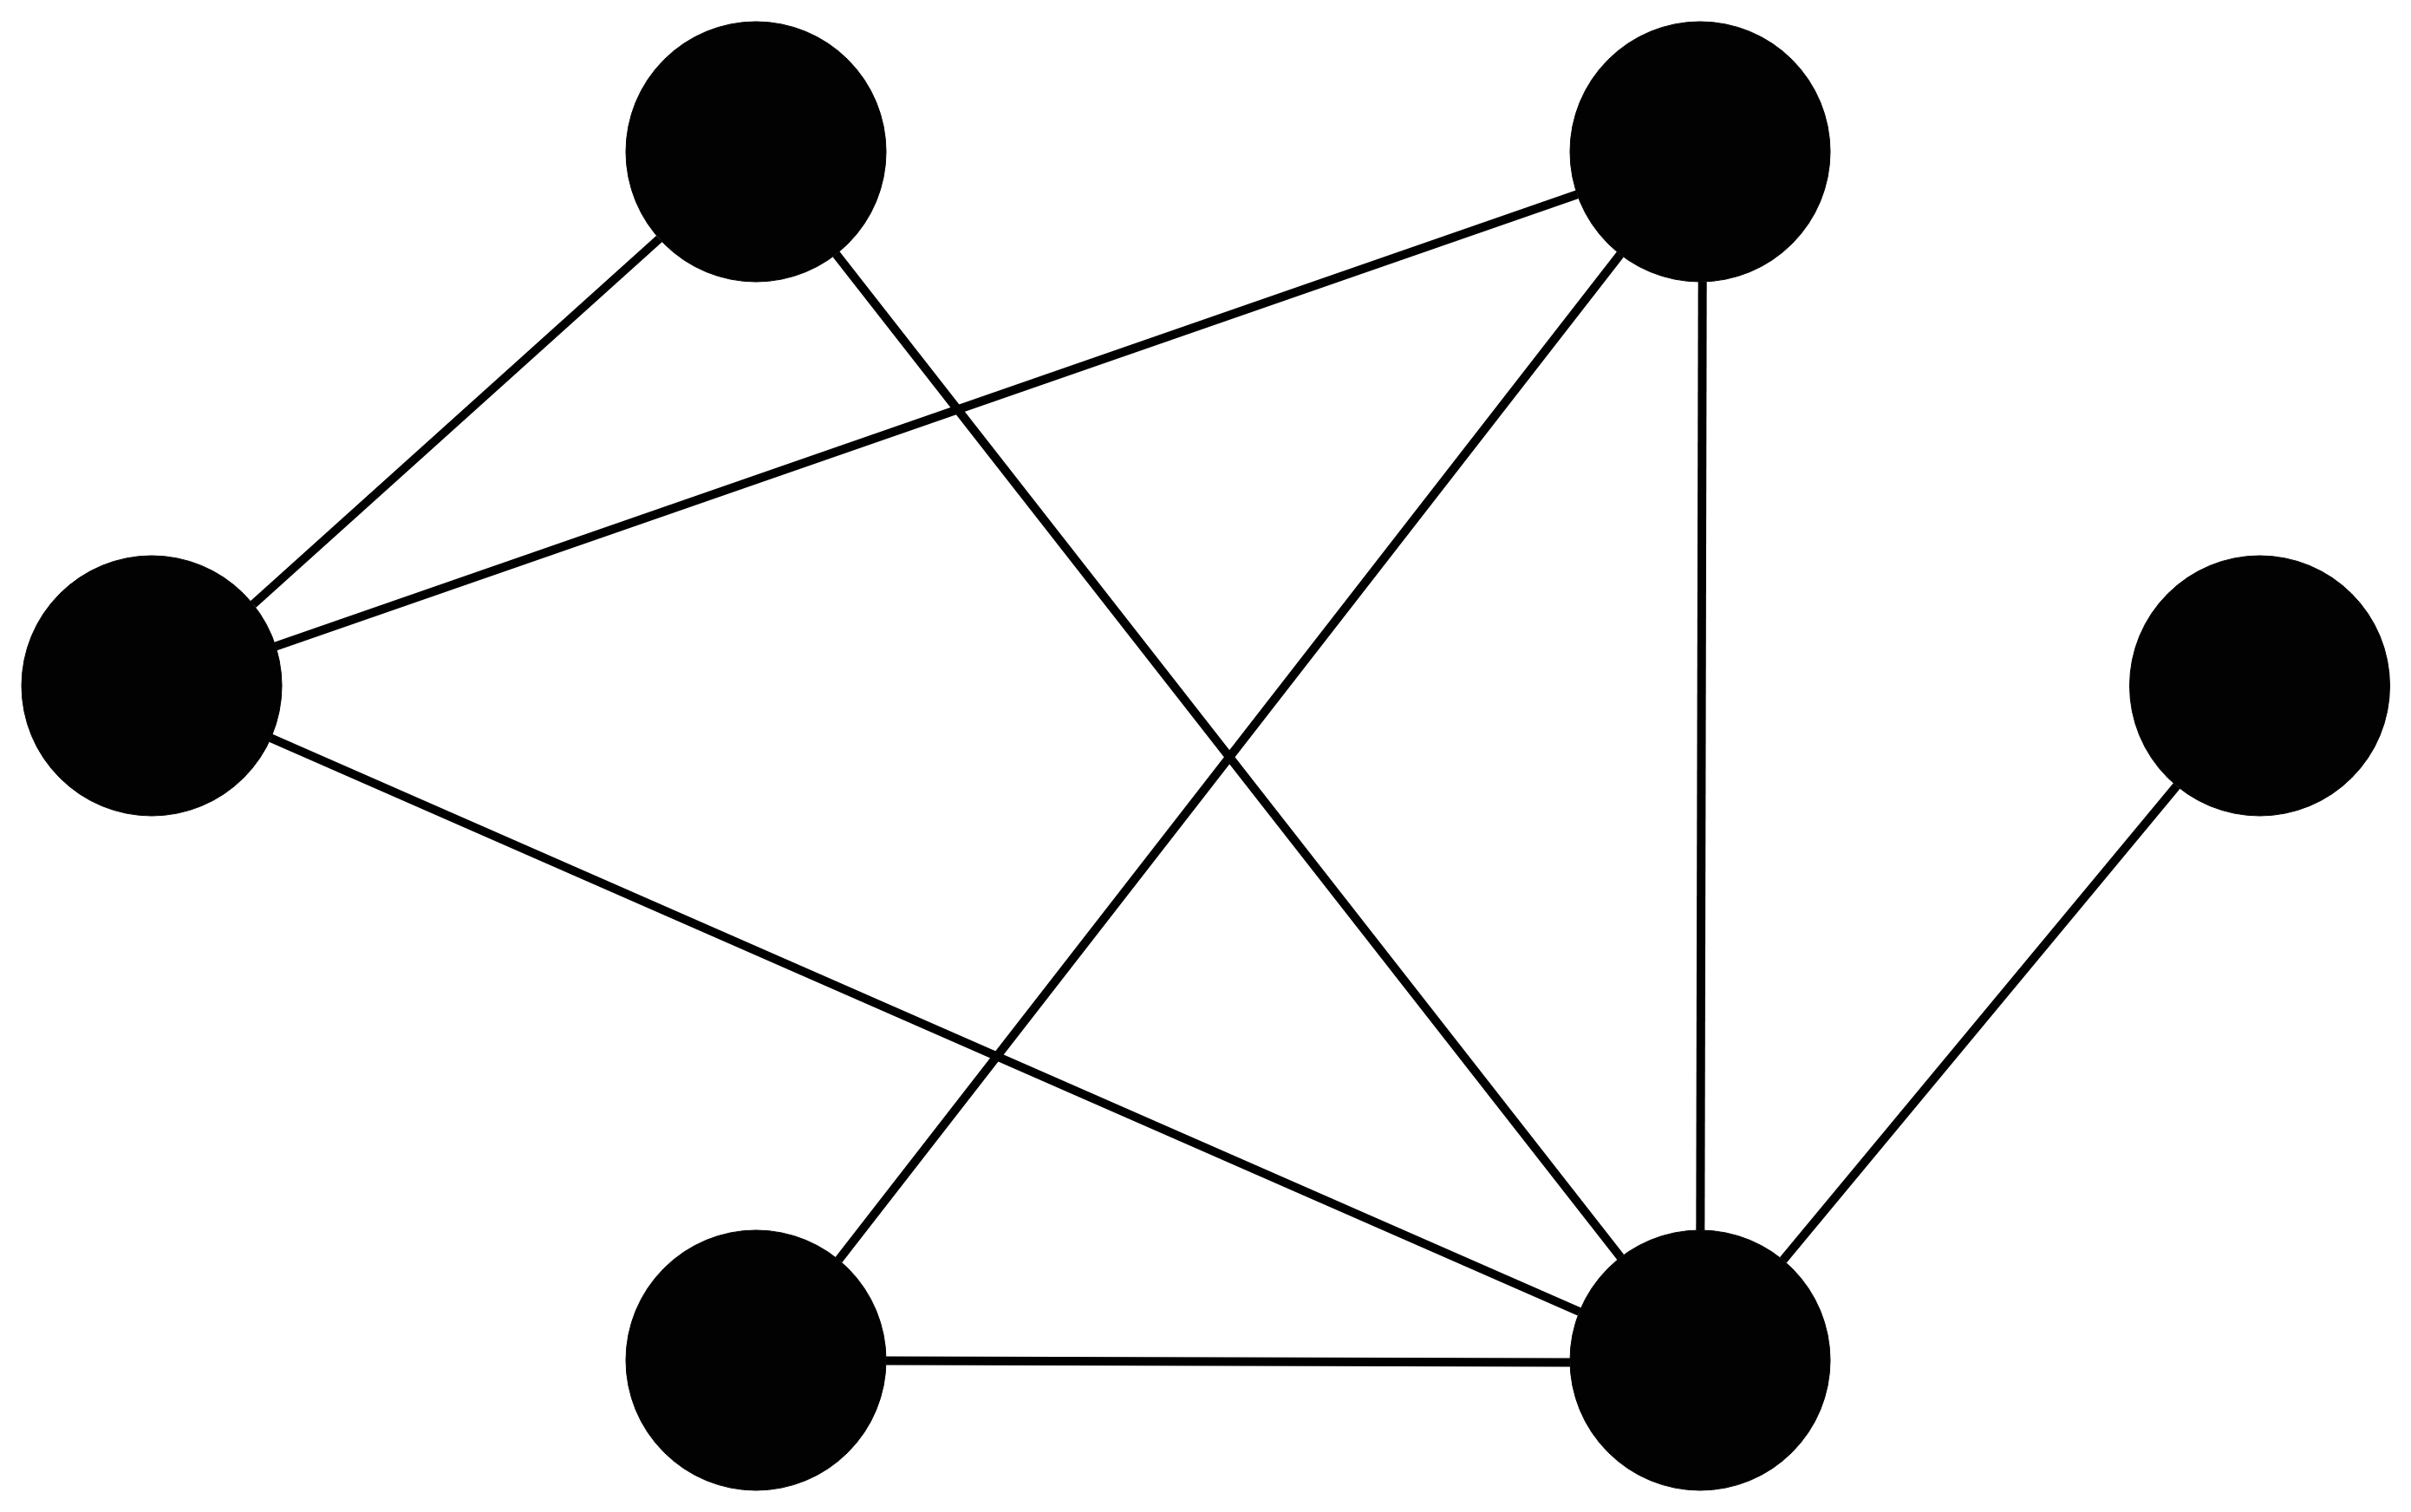
\includegraphics[width=0.6\textwidth]{TCC/imagens/grafos/grafo.png}
     \caption{Representação geométrica de um Grafo}
     \label{Representação geométrica de um grafo}
\end{figure}


Um grafo é comumente representado graficamente conforme a figura \ref{Representação geométrica de um grafo}, onde os vértices são representados por círculos e as arestas por linhas que interligam dois vértices.

Elementos componentes de um grafos conforme definidos por \citeonline{szwarcfiter18} e \citeonline{pinto18} a seguir.


\begin{definition} 
 \textbf{Vértice}: um vértice é denotado por $V(G)$ é representado graficamente através de um ponto, a quantidade dos vértices de um grafo é expressa por $|V|$, onde um grafo com $|V| = 1$ é classificado como um grafo trivial.
 \end{definition}

\begin{definition} 
\textbf{Aresta}: uma aresta $e \in E(G)$ é denotada por um par de vértices $e = (v,w)$. Dessa forma os vértices $v$ e $w$ estão conectados as extremidades da aresta e, dessa forma são denominados adjacentes. Já uma aresta é denominada incidente aos vértices em seus extremos $v$ e $w$.
\end{definition}

\begin{definition} 
\textbf{Grau de um vértice}: o grau de um vértice $v \in V(G)$, é denotado por grau($v$), sendo esse o número de vértices adjacentes a $v$.
\end{definition}

\begin{definition} 
\textbf{Multigrafo}: denotado por $H(V,E)$, é um grafo que admite diferentes arestas incidentes a um mesmo par de vértices $(v,w)$ ou laços, sendo arestas que são incidentes a um único vértice ($v$,$v$).
\end{definition}

\begin{definition} 
\textbf{Grafos Direcionados}: em um grafo direcionado (digrafo) $D(V,E)$ é um conjunto finito não vazio $V(G)$ (os vértices), e um conjunto $E(G)$ (as arestas) de pares ordenados de vértices distintos. Portanto, também que ($v$,$w$) possui uma única direção de $v$ para $w$.
\end{definition}

\begin{definition} 
\textbf{Grafo Ponderado em Arestas}: um grafo é classificado como ponderado quando é atribuído um valor (peso) $p$ as arestas, sendo esse $p(v,w)$ ou $p(e)$.
\end{definition}

\begin{definition} 
\textbf{Rótulo}: um rótulo consiste na atribuição de um valor (numérico ou alfabético) que simbolize ou represente um elemento do grafo de modo a facilitar a identificação de um vértice ou aresta específica em uma representação.
\end{definition}

% Área da matemática muito estudada na computação.
A Teoria dos Grafos é uma área amplamente estudada tanto na matemática quanto na computação. Muitos problemas do mundo podem ser descritos como problemas de grafos, dessa forma, ao se propor uma solução para o modelo de grafos também de obtém a solução para o problema real.

Muitos problemas e soluções já foram propostos com o passar dos anos, isso possibilita que a teoria dos grafos tenha modelos que se adéquem a muitas descrições, e algoritmos (sequência de instruções para se fazer uma operação no computador) eficientes para resolvê-los.

\section{Exemplos de problemas modelados com Grafos}

Atualmente muitos serviços tecnológicos utilizam das estruturas de grafos para resolverem problemas do dia-a-dia das pessoas. Esses serviços podem ser aplicativos para \textit{smartphones}, sistemas \textit{web} ou até mesmo sistemas \textit{desktop}.

Dentre os aplicativos que utilizam de modelos em grafos para resolver seus problemas, destacam-se os seguintes exemplos:


\subsection{\textit{Facebook} e \textit{Twitter}}
    
As mídias sociais que se popularizaram desde a criação da “internet”, muitas podem ter suas aplicações modeladas com uso de grafos, e não apenas isso, mas algumas dessas mídias são criadas de forma a obter benefícios dessas estruturas.

Dois exemplos podem ser destacados pela forma diferente de se utilizar a estrutura dos grafos, o \textbf{\textit{Facebook}} e o \textbf{\textit{Twitter}}. 
    
    O \textit{Facebook} pode ter as relações de amizade representadas como um grafo simples, onde duas pessoas que sejam amigos na plataforma representariam uma relação. Nesse caso cada usuário será representado por um vértice $v \in V$, e usaremos uma aresta ($v$, $w$) para representar relações de amizade entre dois usuários. Como apresentado na figura \ref{grafo-facebook}.
    
    \begin{figure}[H]
         \centering
         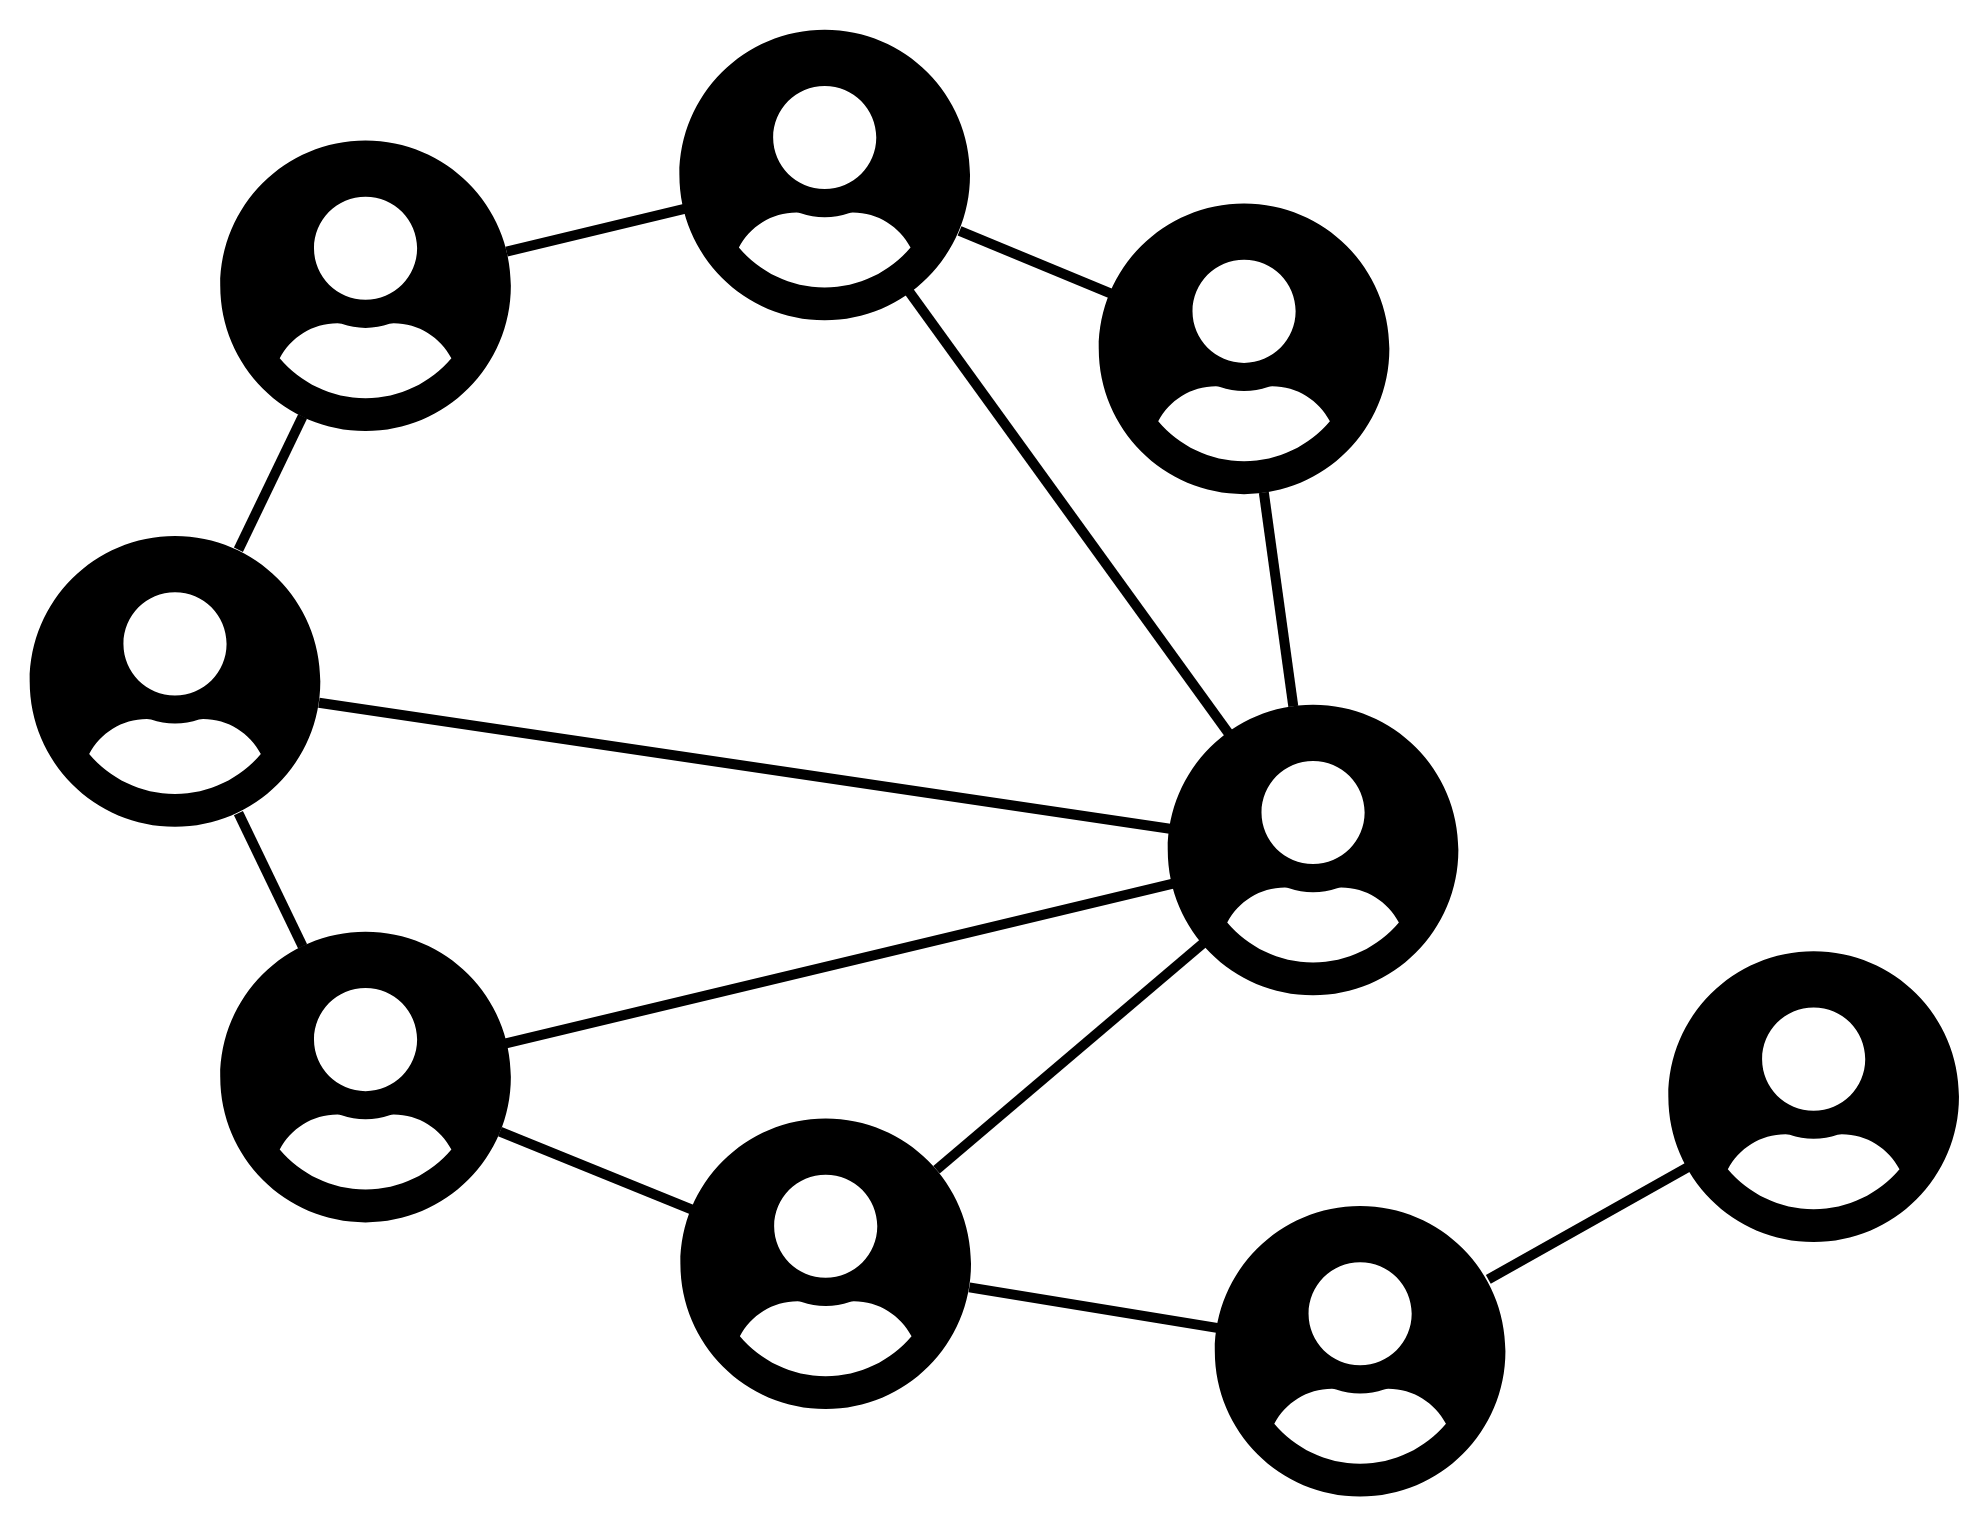
\includegraphics[width=0.6\textwidth]{TCC/imagens/grafos/grafo-facebook.png}
         \caption{Representação de uma rede de amigos do \textit{Facebook} como um Grafo}
         \label{grafo-facebook}
    \end{figure}

Diferente do caso do \textit{Facebook}, onde para termos uma relação de amizade precisamos que os dois usuários sejam amigos entre si, o \textit{Twitter} apresenta o conceito de seguir outros usuários, e não necessariamente ser seguido por eles.

Dessa forma, a representação dessas relações seriam expressas melhor por um multigrafo direcionado, onde os usuários são representados pelos vértices $v$, e uma aresta ($v$, $w$) representará aqueles que ele segue, sendo essas arestas com sentido, com a origem no usuário que segue $v$ e o destino no usuário que é seguido $w$. Dessa forma podemos observar essas diferenças na figura \ref{grafo-twitter}.
    
    \begin{figure}[H]
         \centering
         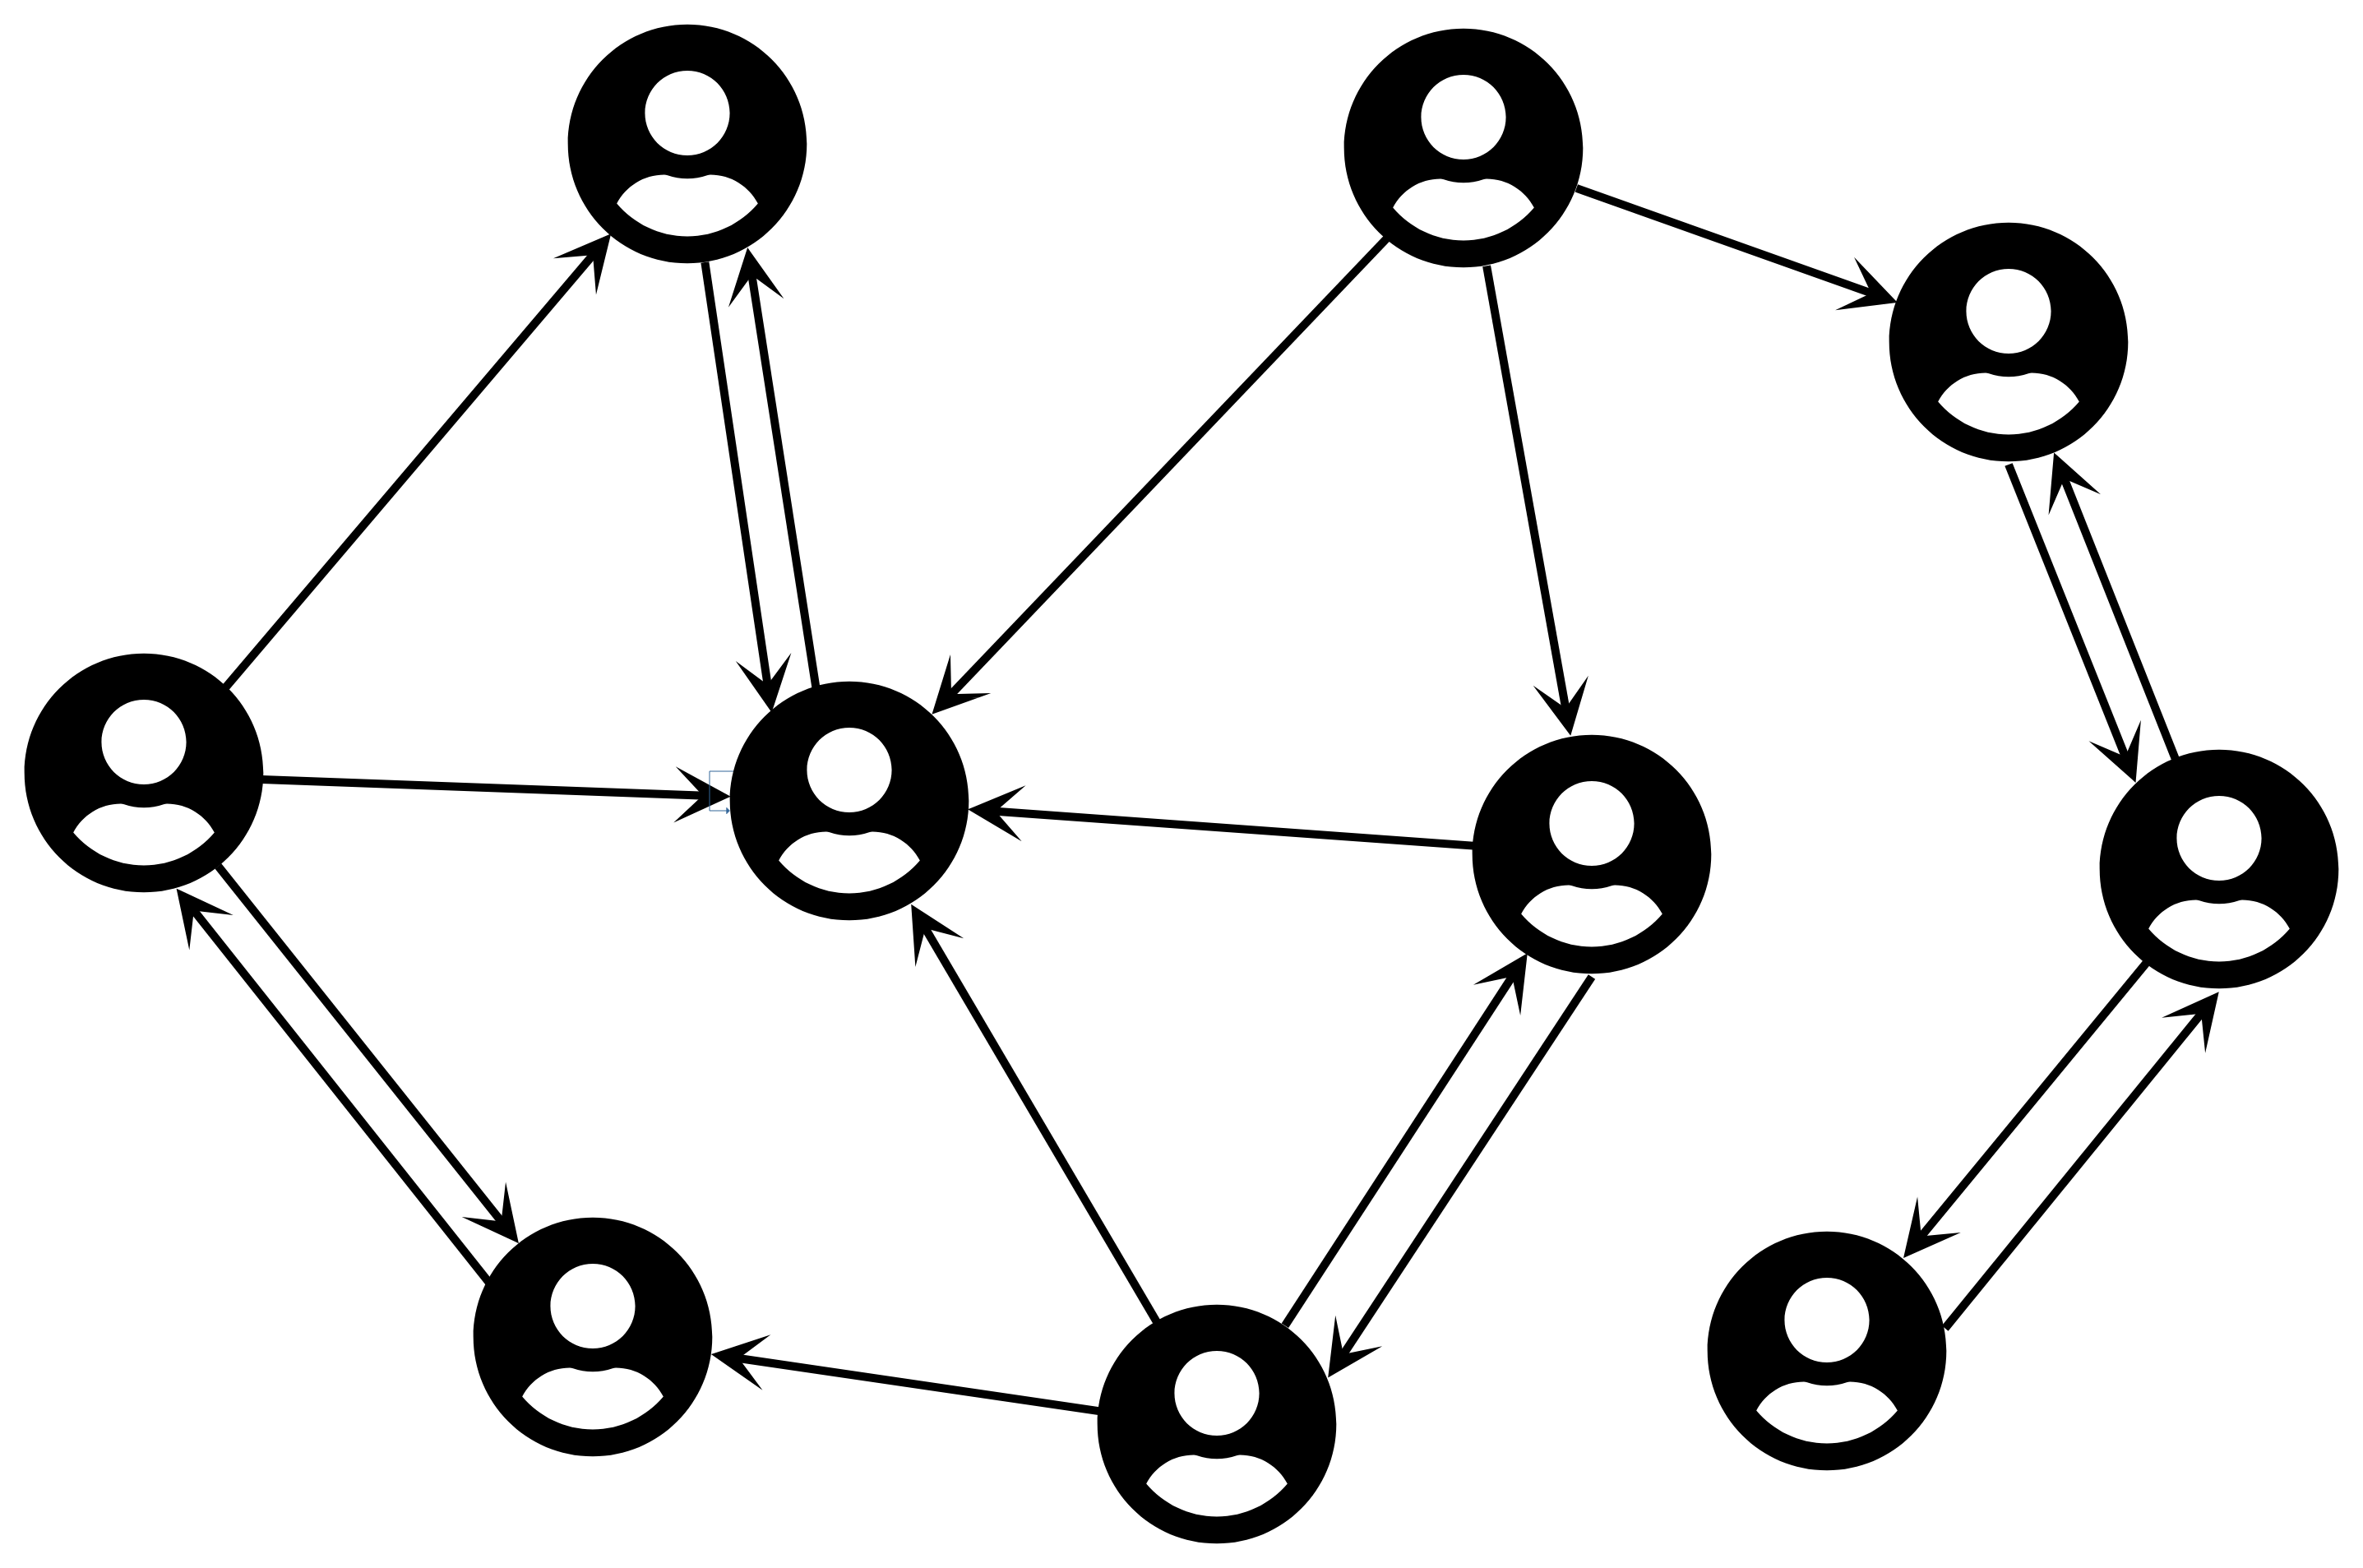
\includegraphics[width=0.6\textwidth]{TCC/imagens/grafos/grafo-twitter.png}
         \caption{Representação de rede de seguidores do \textit{Twitter} como um Grafo}
         \label{grafo-twitter}
    \end{figure}
    
    
    
    \subsection{\textit{Google Maps} e \textit{Waze}}
    
Aplicativos de geolocalização atuais podem utilizar grafos para determinar melhores rotas, podemos considerar como vértices os locais (ou pontos de referência) no qual o usuário deverá passar, e as arestas como o percurso que interligará esses dois pontos.

De acordo com a necessidade, o grafo pode ganhar informações adicionais, como pesos atribuídos as arestas, simbolizando a distância entre dois pontos, ou a velocidade média de outros veículos na travessia entre os dois pontos, esses fatores serão considerados para se propor uma rota, seja a que cruze o menor número de pontos, a que percorra a menor distância total, ou que obtenha a maior velocidade média de modo a percorrer em menor tempo a rota.
    
    \begin{figure}[H]
         \centering
         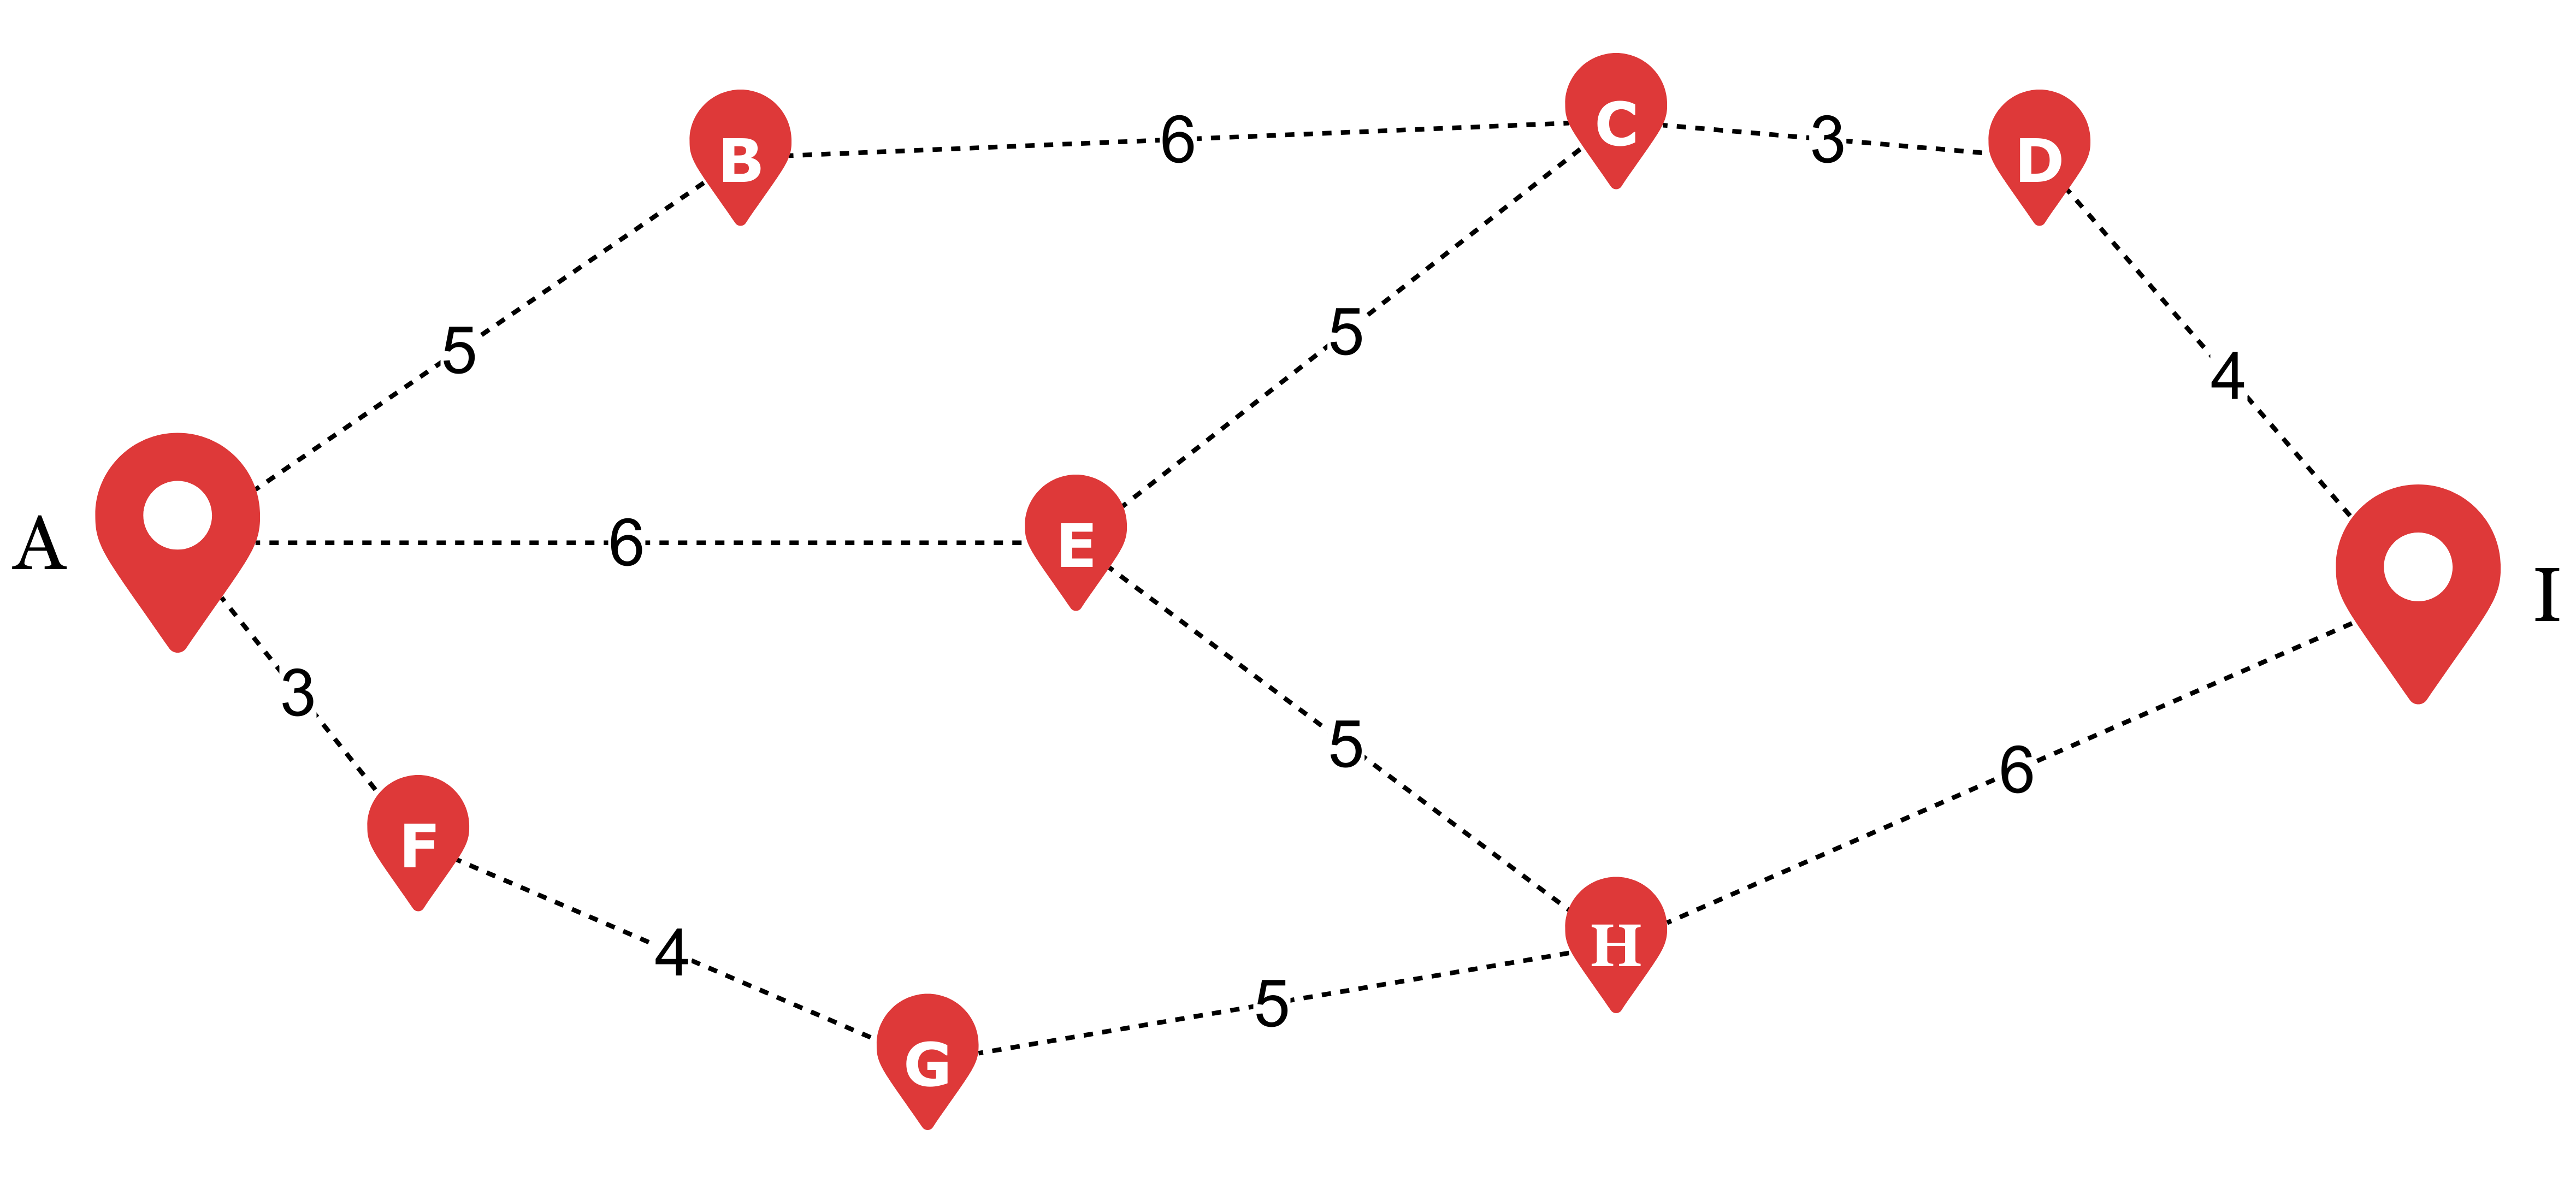
\includegraphics[width=0.6\textwidth]{TCC/imagens/grafos/grafo-maps.png}
         \caption{Representação de mapa de rotas como um Grafo}
         \label{Representação de gráfica de um grafo}
    \end{figure}
 
    
    

    
    




%%
 %%   \section{Definição do Problema Matemático}
 %%   \label{sec:def_prob}
    
 %%    Usando a notação de \cite{goldbarg_05} denotamos como: "Sendo o conjunto $M = \{1, 2, ..., m\}$ e um conjunto $f = \{ M_{1}, M_{2}, ..., M_{n}\}$ uma família de subconjuntos de $M$, onde $ M_j  \subseteq M $ e $ j \in J = \{1, 2, ..., n\} $”.
 %%    Observamos que $M_j \cap M_i \geq 0$, tendo $i \in J$ e $i \neq j$. 
    
%%    Buscando-se particionar os elementos de $f$ em $k$ partes, temos que $P = \{p_1, p_2, ..., p_k\}$ e $P \subseteq f$. 
    
 %%   Busca-se então particionar os elementos de $f$. Sendo $P_{p}$ uma partição $p$ de $\Omega$, com $p \in \{1,...,k\}$. Denotamos $S_p = |\bigcap\limits_{}^{} A'|,\; \forall A ”\in P_{p}$, ou seja, $S_{p}$ é o número de elementos existentes nas interseções entre os conjuntos que pertencem a partição $p$. Definimos também, $S$ como a soma de todos os $S_{p}$ de uma solução, ou: $\sum\limits_{i = 0}^{k}S_{p}$. 
    
  %%  Tendo $ S ”= | \bigcap\limits_{i = 0}^{n} A_{i} |$, e $Q$ um índice de qualidade de uma solução qualquer. Definimos que:
    
 %%   \begin{equation} \label{eq:qualidade}
 %%    Q = \frac{S \times 100}{S'}
  %%  \end{equation}
    
  %%  O objetivo nesse cenário se encontra em obter uma solução que possua o menor valor possível para $Q$, onde 0 seria a solução ótima para o problema, e 100 a pior solução possível. 
    
%%    Uma solução é definida aqui como: um $k$-particionamento qualquer de $\Omega$.
    
    
    % (imagem ilustrativa com N conjuntos de M elementos cada, sendo separada em K partições)
    
    %\subsection{Classificação do Problema}
    
  %%  Ao realizar uma analogia do o problema de \textit{Alocação de Turmas em Horários de Prova}, enunciado em \ref{subsec:desc_prob}, com as definições aqui apresentadas, observamos que: 
    
  %%  \begin{itemize}
  %%  \item[(a)] $\Omega$ corresponderá à uma instituição;
 %%   \item[(b)] um elemento $A_{i} \in f$ será correspondente a uma turma qualquer, onde $i$ representa uma turma específica;
 %%   \item[(c)] uma partição $P$ equivalerá à um horário de prova;
 %%   \item[(d)] e $S$ será o número de provas de segunda chamada necessárias, tendo $S_{p}$ como o número de conflitos obtidos em um horário $p$.  
%%    \end{itemize}
    
    

\section{Grafo de Interseção de Turmas}


\citeonline{pinto18} define um grafo de interseção, quando seja possível esse grafo $G(V, E)$ representar as relações entre elementos de um conjunto através das relações entre seus vértices $v \in V$.

Para modelarmos nosso problema original na forma de um grafo, será necessário ainda ressaltar algumas das características pertencentes ao problema estudado.

Observando uma instituição universitária, suas turmas têm caráter diferente do contexto escolar (ensino fundamental e ensino médio), em uma universidade as turmas são equivalentes uma disciplina que pode ser ofertada a um grupo de alunos, onde esses podem se inscrever nela ou não, de acordo com as normas estabelecidas pela instituição e vontade do aluno.

Um aluno, dessa forma, irá se inscrever em uma série de turmas todo semestre letivo. Cada turma terá ao início de cada semestre uma lista de alunos inscritos.

Para modelar essas turmas em um grafo de interseções, iremos primeiramente observar as listas de alunos inscritos nas turmas da instituição, como no exemplo mostrado a seguir na tabela \ref{tabela-lista-turmas}.

\begin{table}[H]
    \centering
    \vspace{0.5cm}
    \renewcommand\arraystretch{1.5}
    \begin{tabular}{c|c|c|c}
     
        \textbf{Turma A} & \textbf{Turma B} & \textbf{Turma C} & \textbf{Turma D} \\ % Note a separação de col. e a quebra de linhas
        \hline                               % para uma linha horizontal
        001   &   003  &   001   &   020  \\
        002   &   006  &   003   &   021  \\
        003   &   009  &   006   &   022  \\
        004   &   011  &   009   &   023  \\ 
        005   &   012  &   011   &   024  \\ 
        006   &   013  &   012   &   025  \\ 
        007   &   014  &   013   &   026  \\ 
        008   &   015  &   018   &   027  \\ 
        009   &   016  &   019   &   028  \\ 
        010   &   017  &   020   &   029     % não é preciso quebrar a última linha
        \\
        \hline
    \end{tabular}
    \caption{Lista de turmas e a matrícula seus respectivos alunos}
    \label{tabela-lista-turmas}
\end{table}

Observamos que essa instituição possui quatro turmas, com dez alunos em cada turma.

As turmas nesse exemplo são: “turma A', “turma B', “turma C ”e “turma D'. Nesse cenário iremos atribuir um vértice para cada turma, sendo o rótulo do vértice a letra que representa a respectiva turma (A, B, C e D).

Ao realizar esse processo teremos como resultado o grafo da figura \ref{grafo-turmas1}, com quatro vértices, um para cada turma.

\begin{figure}[H]
     \centering
     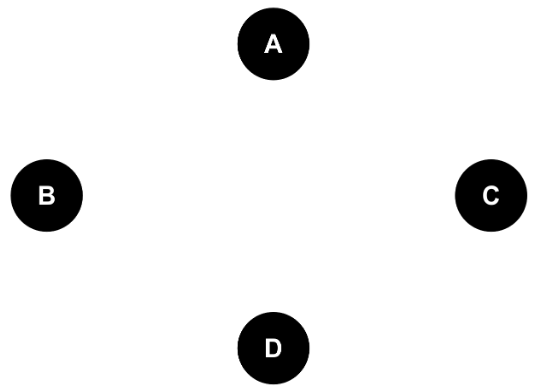
\includegraphics[width=0.4\textwidth]{TCC/imagens/grafos/turmas-vertices1.png}
     \caption{Turmas modeladas como um Grafo}
     \label{grafo-turmas1}
\end{figure}

Foi definido em nossa modelagem que uma aresta representaria a interseção de alunos entre duas turmas. Com isso toda turma que possuir alunos em comum irá receber uma aresta ($e$) que interligue os vértices ($v$ e $w$) referentes as respectivas turmas.

Observando novamente a tabela \ref{tabela-lista-turmas}, ao compararmos os alunos inscritos nas turmas A e B, notaremos que existem alguns alunos que pertencem a ambas turmas, como os alunos \textit{003, 006 e 009}.

Essa interseção observada irá gerar uma aresta no grafo que interliga os vértices \textbf{A} e \textbf{B}, como pode ser visto na figura \ref{grafo-turmas2}. Representando assim que ambas turmas possuem alunos em comum.

\begin{figure}[H]
     \centering
     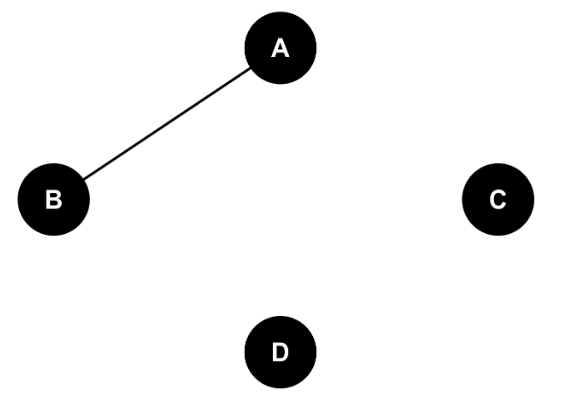
\includegraphics[width=0.4\textwidth]{TCC/imagens/grafos/turmas-vertices2.png}
     \caption{Representação do Grafo após comparar as turmas A e B}
     \label{grafo-turmas2}
\end{figure}

Repetindo o processo de observar a existência de alunos em comum entre cada par de turmas, iremos formar respectivamente os grafos exibidos nas figuras \ref{grafo-turmas3}, \ref{grafo-turmas4} e \ref{grafo-turmas5}.

\begin{figure}[H]
     \centering
     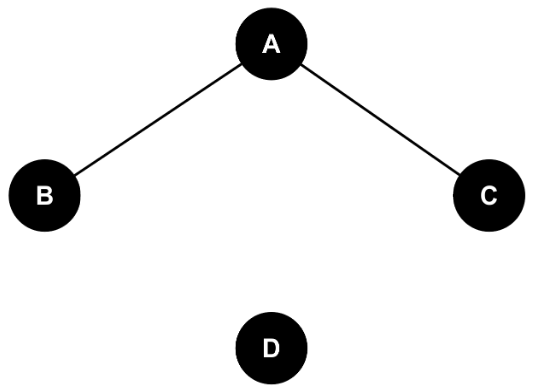
\includegraphics[width=0.4\textwidth]{TCC/imagens/grafos/turmas-vertices3.png}
     \caption{Representação do Grafo após comparar as turmas A e C}
     \label{grafo-turmas3}
\end{figure}

\begin{figure}[H]
     \centering
     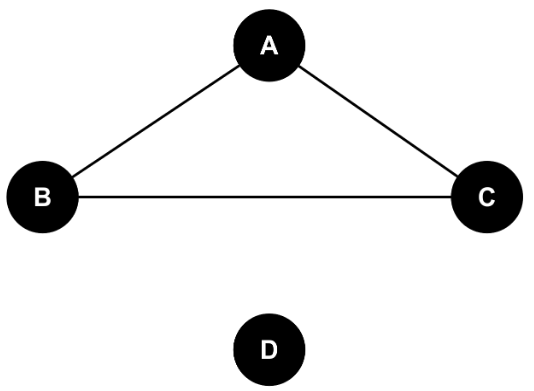
\includegraphics[width=0.4\textwidth]{TCC/imagens/grafos/turmas-vertices4.png}
     \caption{Representação do Grafo após comparar as turmas B e C}
     \label{grafo-turmas4}
\end{figure}

\begin{figure}[H]
     \centering
     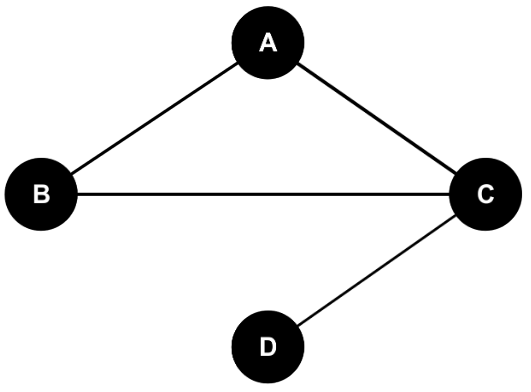
\includegraphics[width=0.4\textwidth]{TCC/imagens/grafos/turmas-vertices5.png}
     \caption{Representação do Grafo após comparar as turmas C e D}
     \label{grafo-turmas5}
\end{figure}

Finalizando o processo de identificação de interseções entre as turmas teremos o grafo de interseção das turmas da instituição, e através dele (figura \ref{grafo-turmas5}), podemos observar todas as turmas que possuem alunos em comum.

Agora que sabemos como transformar um conjunto de turmas em um grafo, precisaremos encontrar um meio de utilizar essa estrutura para simplificar a forma como criaríamos a grade de exames universitários.

A forma pela qual criaremos as grades de horários, será apresentada no capítulo de \ref{cap:solucao}, onde será utilizado o grafo criado no exemplo desse subcapítulo (figura \ref{grafo-turmas5}) para demonstrar os benefícios e limitações provenientes dessa modelagem e suas devidas soluções.





%%
%%
%%
%%


\chapter{Método de Solução}
\pagestyle{simple}
\label{cap:solucao}

Após realizar a modelagem na forma de um problema de grafo, iremos utilizar essa estrutura para criar uma grade de horário de provas que satisfaça as restrições do problema.

Considerando um grafo $G$ qualquer, definimos como as turmas pertencentes á $G$ como $V(G) = \{v_1, v_2, v_3, …, v_n\}$, ou seja, o conjunto de vértices $V(G)$ corresponderá às disciplinas ofertadas na instituição, sendo $n$ a quantidade de vértices do grafo $|V(G)|$ e de disciplinas ofertadas.

Definimos que os horários serão representados por números inteiros positivos $K = \{1, 2, 3, …, k\} \in \mathbf{N}$, sendo $k$ o número correspondente a quantidade máxima de horários para realização das provas.

Ao atribuirmos uma turma a um horário de prova, estaremos relacionando um elemento de $K$ á um vértice $v$ de $V(G)$.

Sendo $V(G) = \{v_1, v_2, v_3, v_4\}$ e $K = \{1, 2, 3, 4\}$, podemos realizar uma atribuição que gere o resultado apresentado na tabela a seguir:

\begin{table}[H]
    \centering
    \vspace{0.5cm}
    \renewcommand\arraystretch{1.5}
    \begin{tabular}{c|c}
     
        \textbf{Vértices ($V(G)$)} & \textbf{Horários ($K$)} \\ % Note a separação de col. e a quebra de linhas
        \hline                               % para uma linha horizontal
        	$v_1$ & 1 \\
$v_2$ & 2 \\
$v_3$ & 3 \\
$v_4$ & 4      % não é preciso quebrar a última linha
        \\
        \hline
    \end{tabular}
    \caption{Relação entre os vértices e os horários}
    \label{tabela-relacao1}
\end{table}




Dessa forma, teremos cada turma realizando a prova em um horário distinto. Como apresentado no capítulo \ref{cap:problema}, esse seria um exemplo de solução trivial para o problema.

Contudo, assim como explicado anteriormente, a solução trivial não é o foco do trabalho, dessa forma para se realizar a atribuição de turmas aos horários deveremos por uma ou mais turmas em um mesmo horário. 

Para definir quais provas poderão ser aplicadas em um mesmo horário, iremos considerar os alunos pertencentes á ambas turmas. Com isso, caso duas turmas não possuam alunos em comum, elas poderão realizar seus exames em um mesmo horário.

Para sabermos se as turmas possuem alunos em comum, realizamos a modelagem das turmas na forma de um grafo (conforme apresentado no capítulo \ref{cap:modelagem}), dessa maneira podemos visualizar a existência de relações de acordo com as arestas do grafo.

Agora, para realizarmos a atribuição das turmas em horários aproveitaremos a forma gráfica do grafo, atribuindo uma cor a cada horário.

Para demonstrar, iremos utilizar o grafo resultante da modelagem no capítulo \ref{cap:modelagem} (figura \ref{grafo-turmas5}), que utilizou como base os alunos e as turmas descritas na tabela \ref{tabela-lista-turmas}.

Caso tivéssemos quatro ou mais horários disponíveis, bastaria realizar a solução trivial para o problema, então definiremos que será necessário aplicar as provas dessas turmas em apenas três horários. Sendo assim, teremos $k = 3$ horários e $n = 4$ turmas.

Para facilitar a visualização das operações que serão realizadas, relacionaremos os horários que temos disponíveis para realização de prova á cores únicas, conforme a tabela abaixo:

\begin{table}[H]
    \centering
    \vspace{0.5cm}
    \renewcommand\arraystretch{1.5}
    \begin{tabular}{c|c}
     
        \textbf{Horário} & \textbf{Cor} \\ % Note a separação de col. e a quebra de linhas
        \hline                               % para uma linha horizontal
        	1 & Vermelho \\
2  & Azul \\
3 & Verde
        \\
        \hline
    \end{tabular}
    \caption{Relação entre horários e cores}
    \label{tabela-relacao2}
\end{table}


A partir disso iremos atribuir á primeira turma o primeiro horário, dessa forma podemos pintar o vértice \textbf{A} (correspondente a turma A) de vermelho (cor que corresponde ao horário 1), assim como pode ser observado na figura \ref{grafo-colorido1}.

\begin{figure}[H]
     \centering
     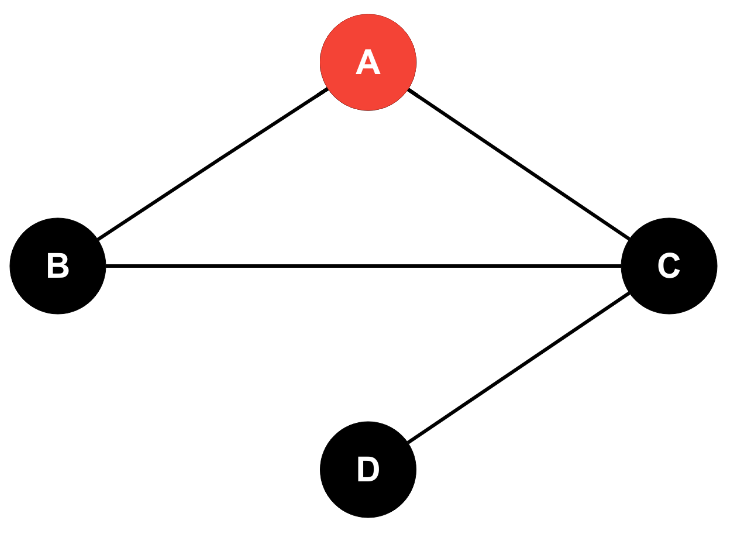
\includegraphics[width=0.4\textwidth]{TCC/imagens/grafos/colorindo1.png}
     \caption{Grafo após definir horário para turma A}
     \label{grafo-colorido1}
\end{figure}


Ao olhar para o vértice \textbf{B}, percebemos que a turma que ele representa possui alunos em comum com a turma representada pelo vértice \textbf{A}, logo, caso ambas as turmas necessitem fazer prova em um mesmo horário, esses alunos em comum terão que obrigatoriamente realizar a segunda chamada de uma das disciplinas.


Assim, visando evitar esse conflito de horários iremos atribuir a “turma B ”ao horário 2, com isso pintaremos o vértice \textbf{B} de Azul.

\begin{figure}[H]
     \centering
     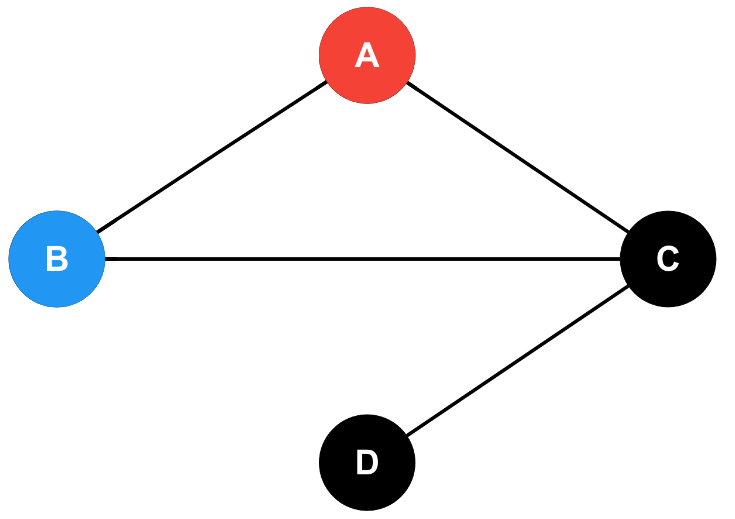
\includegraphics[width=0.4\textwidth]{TCC/imagens/grafos/colorindo2.png}
     \caption{Grafo após definir horário para turma B}
     \label{grafo-colorido2}
\end{figure}


Observando que o vértice \textbf{C} é adjacente (ligado por arestas)
 aos vértices \textbf{A} e \textbf{B}, sabemos que ele possui alunos em comum com ambas as turmas, dessa forma ele não deverá ser colocado em um horário diferente, assim atribuiremos ele ao horário 3 e pintaremos ele de verde.

\begin{figure}[H]
     \centering
     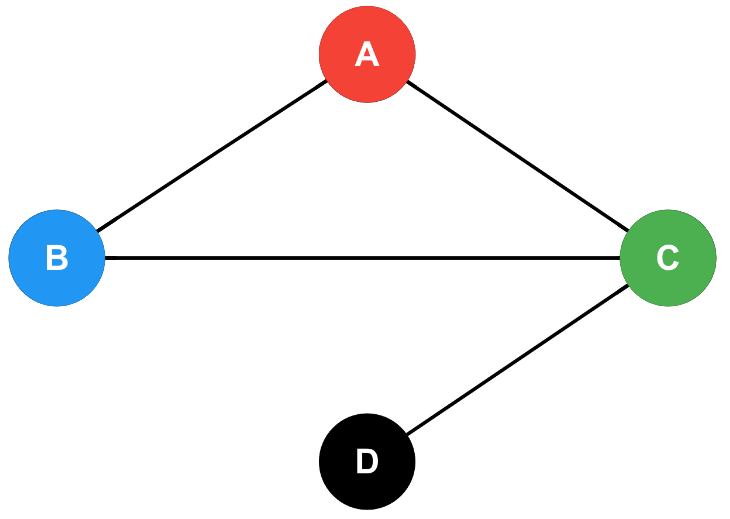
\includegraphics[width=0.4\textwidth]{TCC/imagens/grafos/colorindo3.png}
     \caption{Grafo após definir horário para turma C}
     \label{grafo-colorido3}
\end{figure}


O vértice \textbf{D}, é adjacente apenas ao vértice \textbf{C}, logo poderíamos pinta-lo de vermelho ou de azul, e dessa forma seus alunos realizariam a prova sem conflitos. Iremos então atribuí-lo ao horário 1 no mesmo horário que a turma A, e pintaremos o vértice D de vermelho.

Dessa forma podemos observar na figura \ref{grafo-colorido4} a distribuição das turmas em seus respectivos horários através do grafo com todos os seus vértices pintados.

\begin{figure}[H]
     \centering
     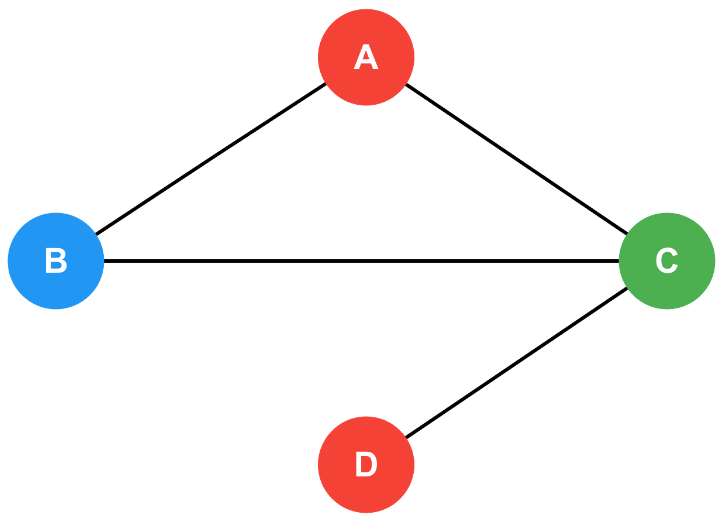
\includegraphics[width=0.4\textwidth]{TCC/imagens/grafos/colorindo4.png}
     \caption{Grafo após definir horário para turma D}
     \label{grafo-colorido4}
\end{figure}

Com isso obtemos como resultado, a grade de horários representada pela tabela a seguir:

\begin{table}[H]
    \centering
    \vspace{0.5cm}
    \renewcommand\arraystretch{1.5}
    \begin{tabular}{c|c}
     
        \textbf{Turmas} & \textbf{Horário} \\ % Note a separação de col. e a quebra de linhas
        \hline                               % para uma linha horizontal
        	A, D & 1 \\
B  & 2 \\
C & 3
        \\
        \hline
    \end{tabular}
    \caption{Alocação das turmas em três horários}
    \label{tabela-relacao3}
\end{table}



O processo de pintar os vértices do grafo, de forma que vértices adjacentes não recebam mesma cor, consiste em uma área muito estudada dentro da Teoria de Grafos, que é a Coloração de Grafos.

No caso específico apresentado, pode ser observado que realizar a alocação das turmas em horários, corresponde á busca por uma coloração própria de vértices do grafo.


\section{Coloração Própria de Vértices de um Grafo}


% [DEFINIÇÃO]

% O que é coloração

A coloração de um grafo qualquer é dada através da atribuição de rótulos aos elementos pertencentes ao grafo (vértices ou arestas), relacionamos esses rótulos à cores de forma a facilitar a visualização da coloração. Contudo para uma coloração ser válida ela precisa cumprir determinada restrição, elementos adjacentes (ou incidentes) não podem possuir mesma “cor”.

% Coloração de vértices

Entre os tipos de coloração existem as de vértices, arestas e total, que visam colorir tanto vértices quanto arestas. Para \citeonline{goldbarg_12} colorir os vértices de um grafo propriamente corresponde a atribuir cores aos vértices de forma que os vértices adjacentes recebam cores distintas.


\begin{figure}[H]
     \centering
     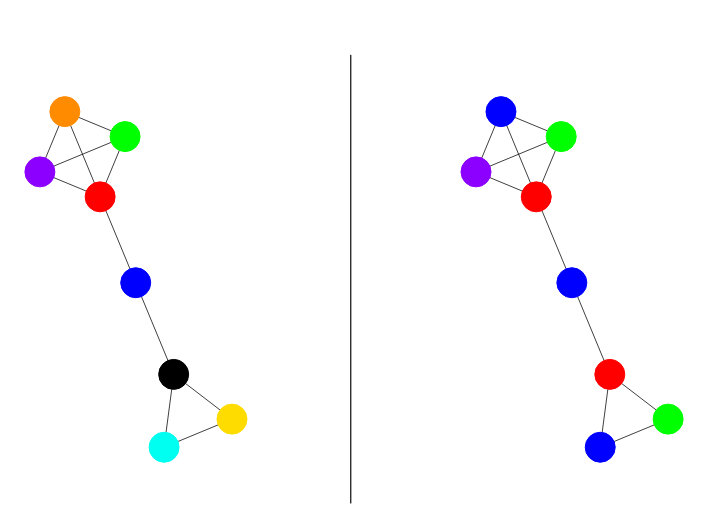
\includegraphics[width=0.4\textwidth]{TCC/imagens/grafos/grafo-propriamente.png}
     \caption{Grafo colorido propriamente}
     \label{grafo-propriamente}
\end{figure}


Uma coloração própria para os vértices de um grafo pode ser realizada ao se colorir cada vértice de uma cor diferente, dessa forma nenhum vértice adjacente (ou vizinho) terá mesma cor. No entanto quando pretendemos colorir os vértices buscando utilizar um número mínimo de cores, nos deparamos com um problema que pode não ser muito simples de se resolver.

% Número Cromático
\begin{definition} 
O menor número possível de cores para se colorir um grafo é chamado de \textbf{número cromático do grafo} denotado por $\chi(G)$. 
\end{definition}

% Coloração própria
Encontrar uma coloração com o número cromático do grafo é classificado como um problema NP-Completo quando $\chi(G) \geq 3$ . Dessa forma, encontrar tal coloração é classificado como um dos problemas mais difíceis estudados na computação.


% [ORIGEM]

Sendo uma das áreas mais estudadas na matemática e computação atualmente, a coloração de grafos se popularizou através da demonstração para uma conjectura existente por mais de um século. O matemático Francis Guthrie conjecturou em 1852 que \textbf{quatro cores eram o suficiente para se colorir um mapa}. Por se tratar de um problema muito difícil a demonstração matemática foi apresentada apenas em 1960 com auxílio do poder computacional \cite{lima_14}.

\begin{figure}[H]
     \centering
     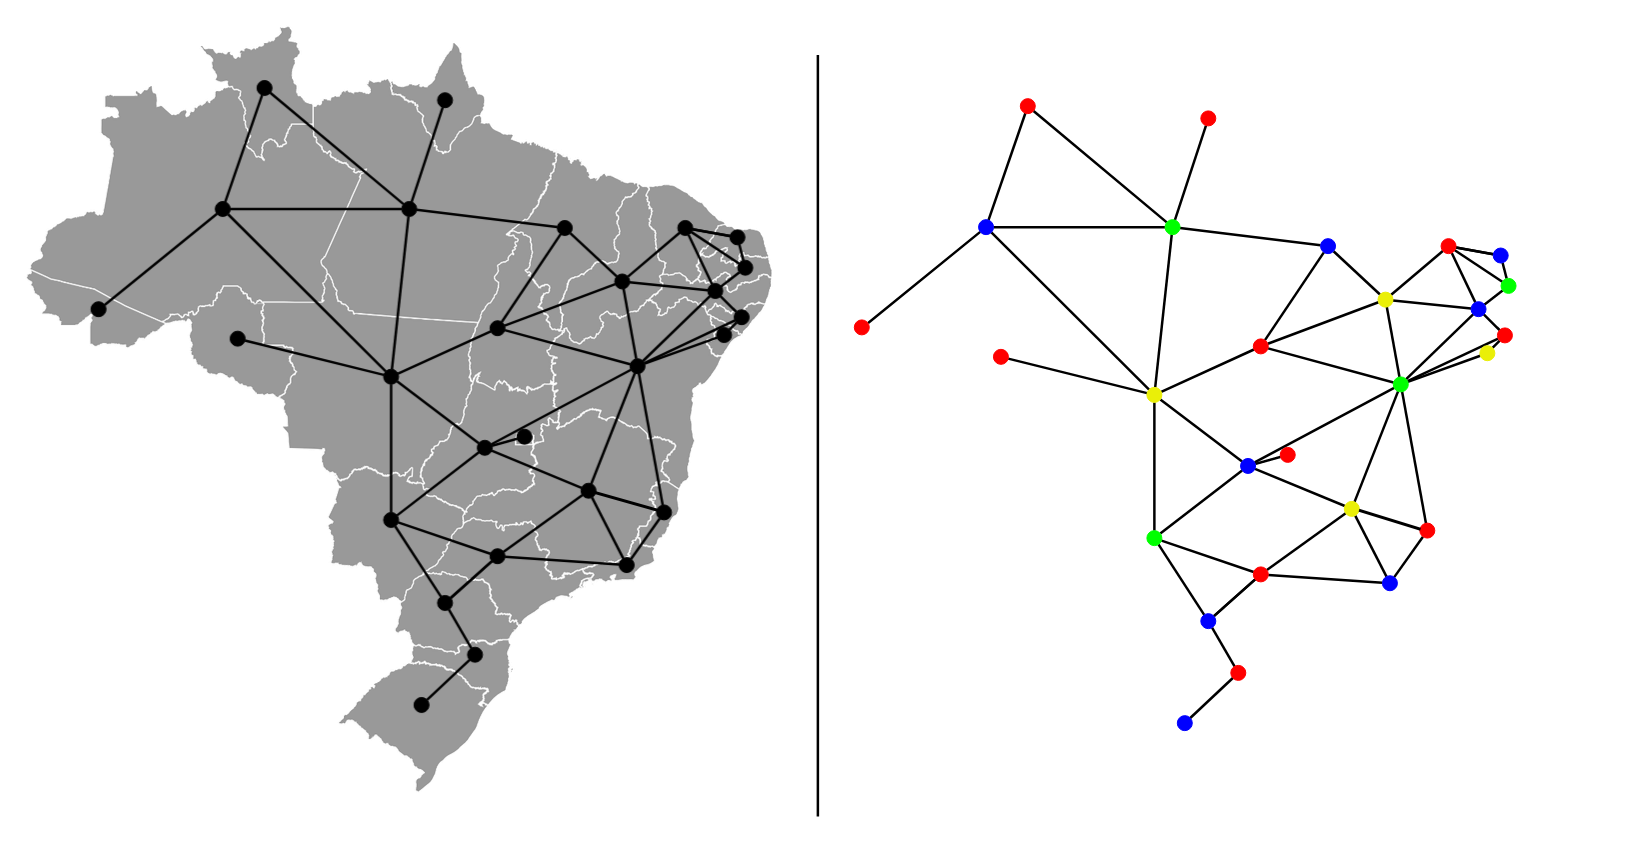
\includegraphics[width=0.8\textwidth]{TCC/imagens/grafos/grafo-mapa4cores.png}
     \caption{Exemplo de 4-coloração do mapa do Brasil}
     \label{grafo-mapa4cores}
\end{figure}

Para essa demonstração foi utilizada uma estrutura de grafo, onde buscava-se modelar um mapa de forma que os vértices representassem locais e esses vértices possuiriam arestas caso possuíssem fronteira. Então ao se colorir propriamente o grafo era possível demonstrar que a mesma coloração poderia ser realizada no mapa, afim de que países que tenham fronteiras em comum não possuam mesma cor.


% [APLICAÇÕES]

Desde então muitos outros modelos e aplicações utilizaram da coloração de grafos como uma forma de solução para um problema abstrato ou concreto.

Além da clássica aplicação concreta da coloração de grafos para se colorir mapas, existem ainda muitas outras formas de se utilizar essa ferramenta matemática.

Algumas aplicações em que se é utilizado a coloração de grafos, e que são formalmente apresentadas em diversos trabalhos e pesquisas acadêmicas, estão formas de se resolver jogos como \textit{SUDOKU}, realização de transporte de componentes que podem ou não se misturados, visando minimizar custos e aumentar a segurança, armazenamento seguro ou inteligente de itens conforme suas características, visando deixa-los mais próximos ou distantes entre muitos outros observados na literatura. 

% [ALGORITMOS]

Existem diversas propostas de algoritmos para encontrar uma coloração própria de um grafo, alguns se destacam por sua simplicidade e desempenho. Desde métodos exatos até heurísticas, as propostas de solução para o problema das colorações são as mais diversificadas possíveis e em alguns casos, a utilização dessas soluções não é o suficiente para se encontrar uma coloração que atenda as condições do problema modelado.

Nesse caso busca-se identificar os fatores que contribuem para a não obtenção do resultado ideal, e assim modelar o problema novamente solucionando então esses possíveis empecilhos.

\section{Limitação no número de Horários de Prova}

A solução do problema de exames universitários por meio da coloração própria de vértices, não resolverá todos os casos possíveis, já que é possível existir um caso onde a quantidade de horários disponíveis para realização da prova $k$ é menor que o número cromático do grafo $\chi(G)$.

\begin{figure}[H]
     \centering
     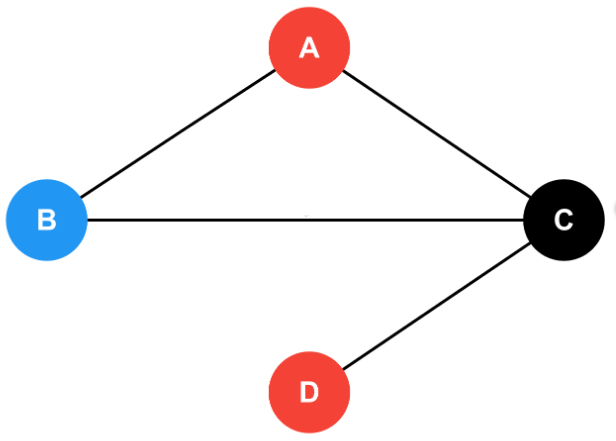
\includegraphics[width=0.4\textwidth]{TCC/imagens/grafos/grafo-colorido-2k.png}
     \caption{Qual cor devo atribuir ao vértice C?}
     \label{grafo-k2}
\end{figure}



Nesse caso, como uma coloração própria não será suficiente, adotaremos uma nova forma de solução. 

Considerando que não será possível separar todas as turmas que possuem alunos em comum em horários de forma que não gere conflitos, iremos buscar uma solução que minimize a quantidade de provas de segunda chamada, ou seja, a número de alunos prejudicados.

Para sabermos quantos alunos estarão sendo prejudicados precisaremos incluir mais uma etapa em nossa modelagem.

Iremos atribuir às arestas do grafo um peso, correspondente a quantidade de alunos que pertencem às duas turmas. Dessa forma teremos um Grafo Ponderado em Arestas.



\section{Grafos Ponderados em Arestas}

Retornando a tabela \ref{tabela-lista-turmas} no capítulo \ref{cap:modelagem}, observamos agora não apenas a existência de alunos em comum às turmas, mas também a quantidade de alunos.

Ao realizar esse processo e escrevermos sobre as arestas a quantidade de alunos na interseção, teremos um grafo ponderado como na figura \ref{grafo-ponderado1}.

\begin{figure}[H]
     \centering
     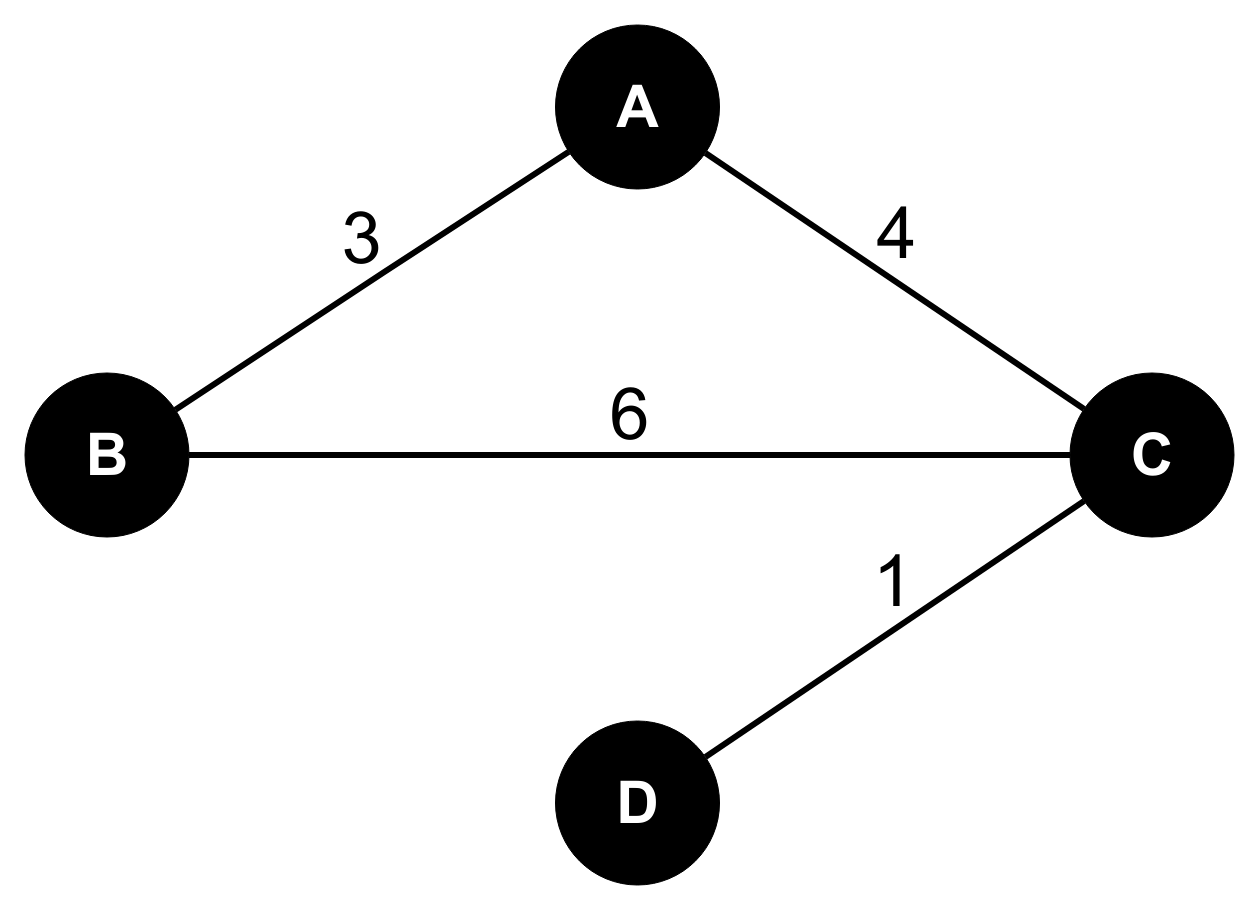
\includegraphics[width=0.4\textwidth]{TCC/imagens/grafos/grafo-ponderado.png}
     \caption{Grafo ponderado em arestas}
     \label{grafo-ponderado1}
\end{figure}


Utilizando do grafo ponderado conseguimos observar quantos alunos seriam prejudicados caso alocarmos quaisquer duas turmas em um mesmo horário. 

Colorir o grafo agora consistirá em encontrar uma coloração não própria cuja soma dos pesos das arestas incidentes em vértices coloridos com mesma cor seja o menor possível.  

Esse processo é chamado de {Generalized Graph Coloring}, onde efetuamos um tipo especial de coloração de modo a atingir algum objetivo pré-estabelecido.




\section{Generalized Graph Coloring Problem}

\begin{definition} 
 \citeonline{vredeveld_02}, define o $k$-GGCP como sendo um problema que consiste em um grafo $G(V, E)$, uma função de peso $z:E \rightarrow  Z$ sobre as arestas, e um número inteiro $k \geq 2$.

Onde deseja-se encontrar uma atribuição de cores $c:V \rightarrow  \{1, ..., k\}$ dos vértices que minimize o peso total das arestas monocromáticas do grafo, isto é, arestas que incidem em vértices com mesma cor.

\end{definition}

Usando o exemplo da figura \ref{grafo-k2}, onde não sabemos como colorir o vértice \textbf{C}, pela ausência de uma terceira cor, iremos testar como seria se escolhermos uma das duas cores para colorir esse vértice.

\begin{figure}[H]
     \centering
     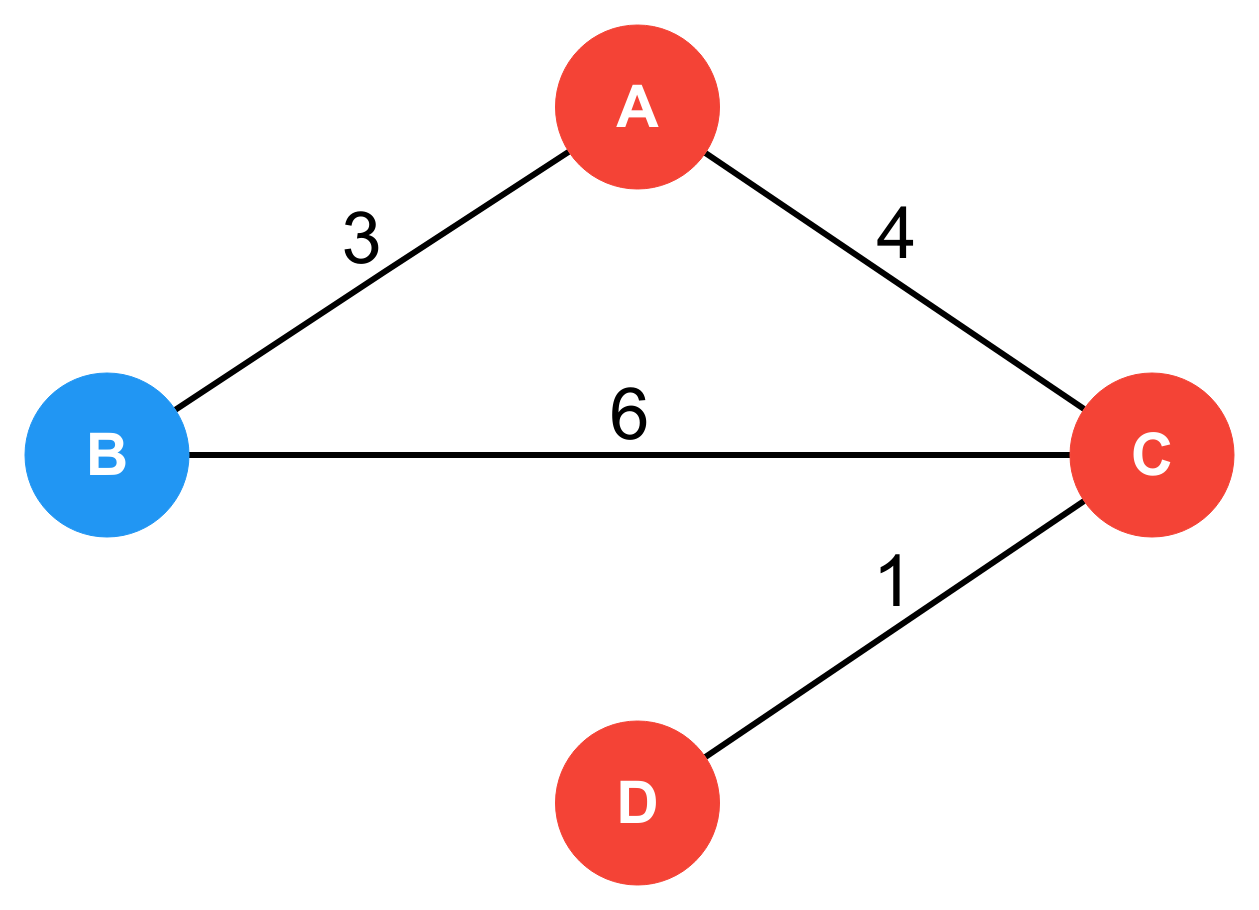
\includegraphics[width=0.4\textwidth]{TCC/imagens/grafos/grafo-ponderado-colorido.png}
     \caption{Caso 1: Grafo colorido com vértice C vermelho}
     \label{grafo-ponderado-colorido1}
\end{figure}


Caso optemos por colorir o vértice \textbf{C} de vermelho, teremos as turmas A, C e D em um mesmo horário de prova. Ao somar o peso das arestas que incidem nesses vértices, temos que cinco provas de segunda chamada serão necessárias, sendo quatro alunos prejudicados nas turmas A e C, e um aluno nas turmas C e D.

\begin{figure}[H]
     \centering
     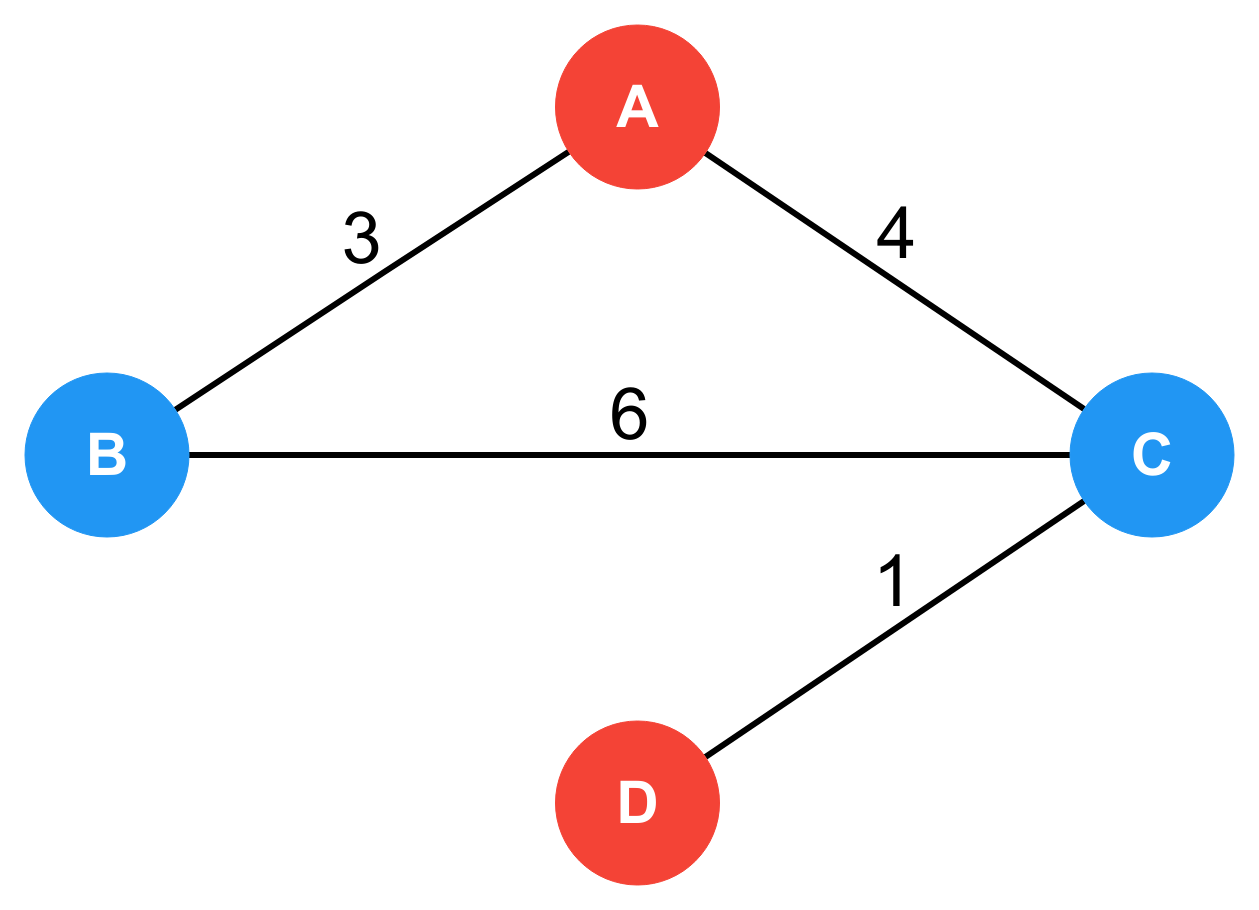
\includegraphics[width=0.4\textwidth]{TCC/imagens/grafos/grafo-ponderado-colorido-v2.png}
     \caption{Caso 2: Grafo colorido com vértice C azul}
     \label{grafo-ponderado-colorido2}
\end{figure}


Escolhendo colorir o vértice de azul, temos a “turma C ”no mesmo horário que a “turma B', o que causaria conflito para os seis alunos que pertencem às duas turmas.

Ao buscar a distribuição que cause o menor número de conflitos chegaremos à coloração representada na figura \ref{grafo-ponderado-colorido3}, no qual podemos observar que teremos apenas os três alunos que fazem parte das turmas A e B prejudicados.

\begin{figure}[H]
     \centering
     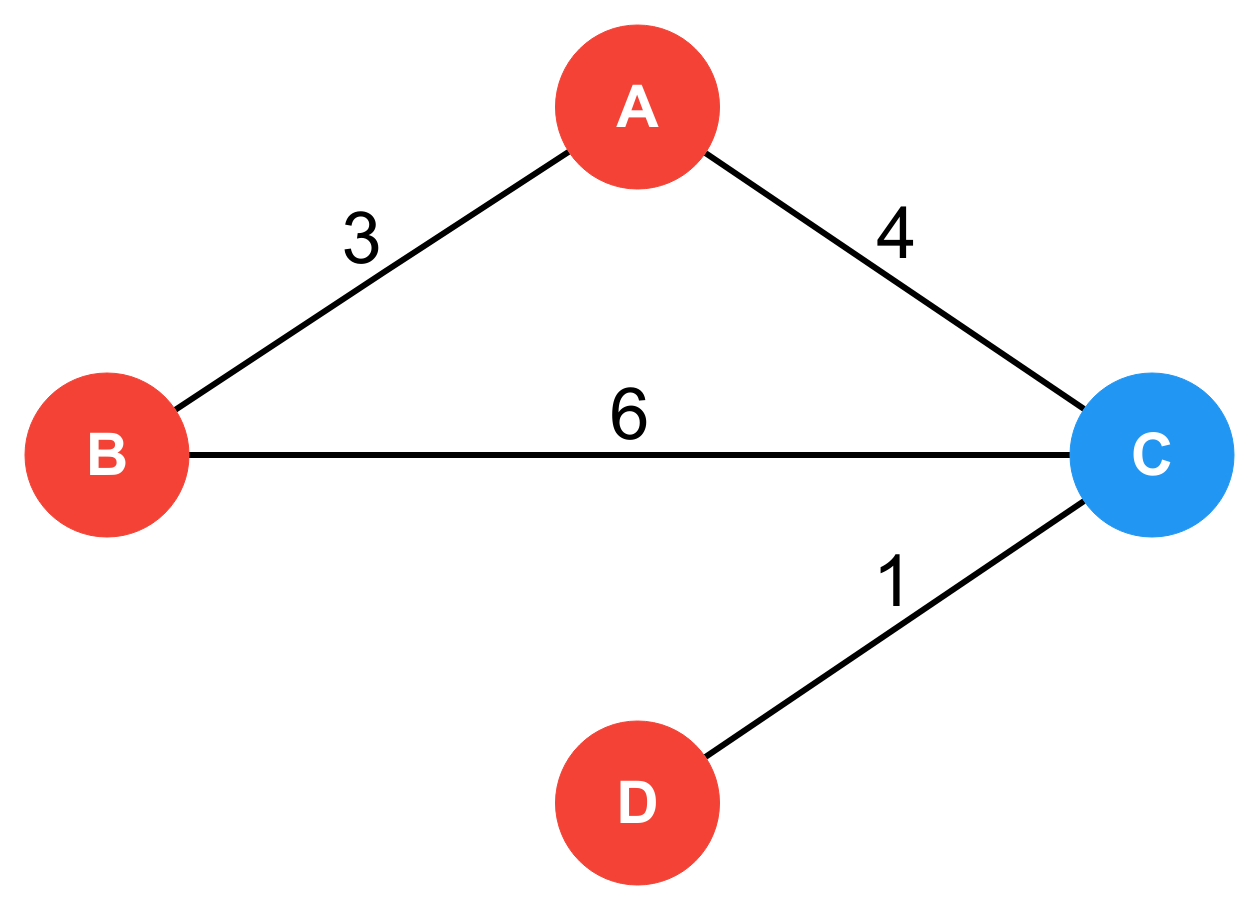
\includegraphics[width=0.4\textwidth]{TCC/imagens/grafos/grafo-ponderado-colorido-v3.png}
     \caption{Melhor coloração com duas cores para o Grafo}
     \label{grafo-ponderado-colorido3}
\end{figure}


Dessa forma o resultado para a grade de horário de prova para as turmas do exemplo será:

\begin{table}[H]
    \centering
    \vspace{0.5cm}
    \renewcommand\arraystretch{1.5}
    \begin{tabular}{c|c}
     
        \textbf{Turma} & \textbf{Horário} \\ % Note a separação de col. e a quebra de linhas
        \hline                               % para uma linha horizontal
        	A, B, C & 1 \\
C  & 2
        \\
        \hline
    \end{tabular}
    \caption{Relação entre horários e cores}
    \label{tabela-relacao4}
\end{table}



Causando dessa forma \textbf{três provas de segunda chamada} por consequência da alocação.



\section{Complexidade do Problema e Viabilidade de Solução}

O PPHC é um problema classificado NP-Completo por \citeonline{garey79}, para todo $k \geq 3$, isso é, para qualquer quantidade de horários maior ou igual a $3$ quando $k$ não for fixo, \citeonline{vredeveld_02} define o problema como NP-Difícil quando o valor $k$ é fixo, por ser equivalente ao MaxCut quando $k = 2$ e equivalente ao problema Max $k$-Cut para qualquer $k \geq 3$, enquanto estes são classificados como NP-Difícil.  

% O problema foi resolvido utilizado o método de força bruta, onde se busca exaustivamente por todas as situações possível a fim de encontrar a melhor solução (cite).

% [O que é NP-Completude e NP-Completo]


Na teoria da computação a complexidade de um problema está diretamente atrelada a capacidade que temos de soluciona-la computacionalmente e o tempo que custará para isso. A maioria dos problemas podem ser divididos em duas diferentes classes P e NP. 

São considerados P os problemas que possuem pelo menos um algoritmo capaz de resolve-lo em tempo polinomial, já um problema NP é um problema não determinístico, porém que pode ter uma solução verificada em tempo polinomial.

% (Pegar definição resumida de problema NP-Completo)
Um subconjunto dos NP é chamado de NP-Completo, sendo uma classe de problemas em que para se pertencer a ela, o problema deve ser classificado como NP e deve ser possível equipara-lo a outro problema já classificado como NP-Completo, ou seja, por definição os NP-Completos são uma classe que ao se encontrar uma solução para um dos problemas os demais também serão solucionados devido a suas semelhanças.

% [O que é um problema NP-Difícil]
Outro subconjunto dos NP são os NP-Difíceis, que são classificados como problemas pelo menos tão difíceis quanto os NP-Completos.


% [O que um problema NP-Difícil interfere na solução]

Ao se deparar com situações desse tipo, o mais comum na literatura é buscar soluções não exatas. Assim, muitos trabalhos publicados para problemas similares ao apresentado aqui, demonstraram bons resultados utilizando diversas técnicas não exatas para se encontrar uma solução, com uso de heurísticas e meta-heurísticas como: \textit{GRASP}, \textit{Busca Tabu}, \textit{Algoritmos Genéticos}, entre muitos outros \cite{rocha13}.

\section{Algoritmo Desenvolvido Inicialmente}
\label{sec-alg-desv}

Um algoritmo foi desenvolvido inicialmente, visando encontrar a melhor alocação de turmas em uma quantidade limitada de horários.

Esse algoritmo possui como entradas: 
\begin{itemize}
    \item[(A)] Um Grafo de interseção ponderado nas arestas $G$;
    \item[(B)] a quantidade $k$ de horários de prova disponíveis.
\end{itemize}
 

E como saída:
\begin{itemize}
    \item[(C)] A coloração $c$  (ou $c^{min}$) com menor custo obtido;
    \item[(D)] a quantidade $P_c$ de provas de segunda chamada necessárias com a coloração de menor custo. 
\end{itemize}
 

A entrada e a saída gerada pelo algoritmo consistia em arquivos de texto e o algoritmo apresentou bons resultados para uma série de testes que foram efetuados.

O método pelo qual o algoritmo buscava a melhor solução consistia em uma busca exaustiva por força bruta, na qual todas as combinações possíveis eram testadas e tinham seus resultados comparados, de modo a encontrar a solução com menor valor $p$ de provas de segunda chamada.

Apesar da garantia da obtenção de uma solução ótima para o problema, o custo computacional (e tempo de processamento) eram muito elevados para grandes instâncias com muitos horários de prova. Visando encontrar uma solução mais viável para grandes instâncias foi proposta a criação de uma heurística que nos permitisse encontrar uma solução boa com menor custo computacional.

\section{Heurística Proposta}


Para desenvolver a heurística foi utilizado como base o bem conhecido algoritmo chamado LF (\emph{Largest-first}), também chamado de método heurístico guloso de coloração própria de vértices de um grafo.

Esse algoritmo foi proposto inicialmente por \citeonline{welsh-powell67} e se baseia na estratégia de escolher colorir primeiramente os vértices que possuem maior grau, ordenando os vértices de acordo com o grau e os colorindo seguindo essa sequência.


\begin{figure}[H]
     \centering
     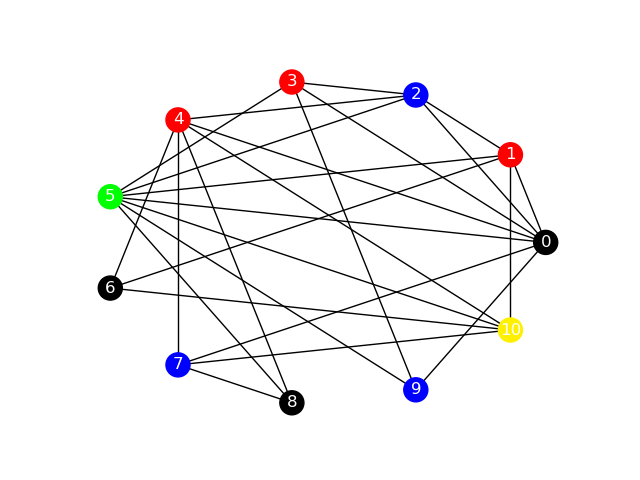
\includegraphics[width=0.7\textwidth]{TCC/imagens/grafos/20_11_50_10_6.png}
     \caption{Exemplo de Grafo colorido com algoritmo inicial }
     \label{grafo-20_11_50_10_6}
\end{figure}


\noindent\begin{minipage}{\linewidth}
\lstset{numbers=left, numberstyle=\tiny, stepnumber=1, numbersep=15pt}

\lstinputlisting[frame=tb,caption=Implementação do LF em Python,
  captionpos=b,belowcaptionskip=2cm, xleftmargin=5.0ex,
  label=zebra,language=python,label={alg-welsh-powell}]{arquivos/welsh-powell.py}
\end{minipage}

O algoritmo apresentado em \ref{alg-welsh-powell} foi desenvolvido inicialmente buscando encontrar colorações onde a quantidade de horários de provas disponíveis eram maiores ou iguais ao número cromático do grafo $\chi(G)$. Porém, conforme o problema evoluiu para um cenário onde deseja-se encontrar uma solução que satisfaça também modelos onde a quantidade de horários disponíveis seja menor que o número cromático do grafo, foi necessário uma mudança na estratégia.

Ao implementar o método por busca exaustiva citado na seção \ref{sec-alg-desv},  notou-se a necessidade de se obter uma solução em um menor tempo de processamento, ao se observar que em modelos com muitas turmas e muitos horários esse tempo de execução poderia dificultar ou até impossibilitar a utilização da mesma.

Foi então proposto um algoritmo adaptado do LF, observado a seguir, onde seria priorizada a coloração com diferentes cores dos vértices adjacentes as arestas de maior peso do grafo, ao invés do vértice de maior grau, como no algoritmo clássico de \citeonline{welsh-powell67}.

O algoritmo proposto pode ser exemplificado através dos passos apresentados através da tabela a seguir.


\begin{table}[H]
    \centering
    \vspace{0.5cm}
    \renewcommand\arraystretch{1.5}
    \begin{tabular}{c|l}
     
        \textbf{Passo} & \textbf{Ação} \\ % Note a separação de col. e a quebra de linhas
        \hline                               % para uma linha horizontal
        	1 & Buscar a aresta $vw$ com maior peso do Grafo, \\ & cujo o vértice $v$ ou $w$ não possuam cor. \\
            2  & Verificar se o vértice $v$ possui uma cor. \\
            3  & Selecionar uma cor $i$ para colorir o vértice $v$. \\
            4  & Verificar se o vértice $v$ pode ser colorido com a cor $i$. \\
            5  & Colorir o vértice $v$ com a cor $i$. \\
			6  & Verificar se o vértice $w$ possui uma cor. \\
            7  & Selecionar uma cor $j$ para colorir o vértice $w$. \\
            8  & Verificar se o vértice $w$ pode ser colorido com a cor $j$. \\
            9  & Colorir o vértice $w$ com a cor $j$. \\
            10 & Repetir o \textbf{passo 1} para a próxima aresta até que \\ & todos os vértices estejam coloridos.
        \\
        \hline
    \end{tabular}
    \caption{Passos para serem executados pela heurística}
    \label{tabela-heuristica}
\end{table}

A cada interação um novo par de vértices $uv$ são selecionados e duas cores são escolhidas para colori-los, contudo em caso de um resultado positivo o ao executar o passo 2 o algoritmo deverá pular para o passo 6. 

Caso não seja possível colorir um vértice com determinada cor, em função dele ser adjacente a outro vértice de mesma cor, o algoritmo deve retornar ao passo anterior e selecionar uma nova cor, se não houverem cores disponíveis o vértice será colorido om a cor que incide na aresta de menor peso.

A seguir está o código em linguagem C que tem como objetivo implementar os passos da heurística a fim de encontrar uma coloração ótima em um tempo reduzido de execução em comparação com o método de busca exaustiva.

\vspace{15pt}

\lstset{ numbers=left, numberstyle=\tiny, stepnumber=1, numbersep=15pt}

\lstinputlisting[frame=tb,caption=Heurística Proposta em C,
  captionpos=b,belowcaptionskip=2cm, xleftmargin=5.0ex,
  label=zebra,language=c,label={heuristica-proposta}]{arquivos/heuristica-proposta.c}

Após desenvolver um modelo no qual pudéssemos representar as turmas e as relações de interseção de alunos entre elas, buscamos então demonstrar um algoritmo capaz de solucionar os desafios apresentados ao longo do capítulo de forma a gerar uma programação de horários de prova com mínimos conflitos de horários de prova para os alunos e consequente aplicação de avaliações de segunda chamada.

Contudo, para possibilitar uma utilização mais diversificada da solução. Foi proposto um sistema, que será apresentado no capítulo \ref{cap:software}, no qual um usuário com menor conhecimento técnico fosse capaz de gerar grades de horários de prova.
 
	% \include{capitulos/mod_mat}

	%\part{Informações Técnicas do Software}
    \chapter{Software para Agendamento de Horários de Provas}
\pagestyle{simple}
\label{cap:software}

Para solucionar o problema apresentado no capitulo \ref{cap:problema}, este trabalho irá apresentar uma proposta de “software” que ofereça ao usuário a possibilidade de se agendar horários de prova, de forma simples e obtendo informações necessárias referentes a solução gerada.

Foi definido como objetivo do desenvolvimento, a criação de um “software” que atendesse as seguintes definições:
\begin{enumerate}
    \item[I --] \textbf{Simplicidade}
    
    Buscando ter um sistema que atenda a simplicidade definida por \citeonline[p. 341]{pressman11} como um conteúdo informativo, sucinto, apropriado para as informações entregues. É dito ainda que esse conteúdo deve apresentar uma estética agradável sem exageros, ter sua arquitetura centrada em atender os objetivos da aplicação da maneira mais simples possível e ter uma navegação de forma intuitivamente óbvia.
    
    \item[II --] \textbf{Compatibilidade}
    
\citeonline[p. 342]{pressman11} define como compatibilidade a necessidade da aplicação de ser usada em uma variedade de ambientes distintos (equipamento físico diferentes, categorias de conexão com “internet”, sistemas operacionais, navegadores) e que a mesma deve ser compatível com esses diversos ambientes.
    
    \item[III --] \textbf{Navegabilidade}
    
 A navegação nas páginas deve ser mantida de forma simples, e previsível para \citeonline[p. 342]{pressman11}, visando propiciar ao usuário um comportamento consistente. Os links devem ser sinalizados, e estarem posicionados de forma a facilitar o acesso aos recursos que esses forneçam.
    
    \item[IV --] \textbf{Reusabilidade}
    
Para \citeonline[p. 362]{pressman11} deve-se pensar o sistema de forma a se permitir a reusabilidade, sendo importante por possibilitar a reutilização do programa, ou de parte dele em outras aplicações.  
    
\end{enumerate}


\section{Tecnologias Utilizadas no Desenvolvimento}

\citeonline[p. 35]{pressman11} define como um sistema “web”, uma categoria de “software” centralizada em redes, sendo em sua forma mais simples um conjunto de arquivos de hipertexto interconectados.

Um sistema “web” pode ser dividido em duas partes, chamadas de “Frontend” e “Backend”. \citeonline{mariosouto2019} classifica “frontend” como sendo a parte visual de um sistema, com a qual um usuário pode interagir, e classifica “backend” como a parte do sistema responsável por realizar a ponte entre os dados no navegador e o banco de dados, aplicando regras de negócio e validações, para garantir o acesso às funcionalidades do sistema.

As tecnologias usadas para desenvolver o “Frontend” do protótipo foram:
\begin{itemize}
    \item[] \textbf{HTML 5}   
    
    \begin{citacao} 
    HTML é uma abreviação de “Hypertext Markup Language” - Linguagem de Marcação de Hipertexto. Resumindo em uma frase: o HTML é uma linguagem para publicação de conteúdo (texto, imagem, vídeo, áudio e etc) na Web \cite{ferreiraHTML}.
    
    \end{citacao}     
    A partir da versão 5 muitos novos recursos foram desenvolvidos e disponibilizados, possibilitando maior utilização de elementos visuais na página com uso de apenas HTML.
       
    \item[] \textbf{CSS 3}
    
     O CSS ("Cascading Style Sheet” ou Folhas de Estilo em Cascata em português) é definido por \citeonline{arianegoncalves2019} como uma linguagem de marcação para estilizar páginas HTML.

Em sua versão 3 o CSS se tornou ainda mais compatível com os navegadores moderno e em conjunto do HTML5 possibilitam a criação de elementos que antes seriam necessárias a inclusão de outras linguagens para realização.
   
   
    \item[] \textbf{JavaScript }
      
   O JavaScript é definido por \citeonline{vilsonheckjunior2014} como uma linguagem de “Scripts” que reside dentro de um documento em HTML, promovendo diferentes níveis de interatividade entre o usuário e a página Web, através da Lógica de Programação.

   
    \item[] \textbf{Cytoscape.JS}
    
    É uma biblioteca que utiliza a Teoria dos Grafos escrita em JavaScript de código aberto que permite a visualização, análise de estruturas de Grafos, com elementos animados.
  
   
    \item[] \textbf{Bootstrap}
    \begin{citacao} 
     Bootstrap é uma biblioteca de “frontend” livre e de código aberto para a criação de sites e aplicações “web”. Ele contém HTML e modelos de “design” baseados em CSS para tipografia, formas, botões, navegação e outros componentes da “interface”, bem como extensões JavaScript opcionais. O Bootstrap destina-se a facilitar o desenvolvimento de sites dinâmicos e aplicações “web” \cite{portalgsti2020}.
    
    \end{citacao}    
    
   Com a utilização do Boostrap é possível ter benefícios para o desenvolvedor quanto para o usuário, para o desenvolvedor existirá um padrão que agilizará o desenvolvimento do “software”, para o usuário as páginas possuirão elementos que lembram elementos que ele já utilizou (visualizou) em outras páginas “Web”.
   
\end{itemize}

As tecnologias usadas para desenvolver o “Backend” do protótipo foram:
\begin{itemize}
    \item[] \textbf{PHP 7.0}
       
    PHP (PHP: “Hypertext Processor”) é uma linguagem de “scripts” de código aberto, que se caracteriza por ser embutido em páginas HTML e executado no lado do servidor, sendo usada principalmente para realização de conexões com banco de dados. 
   
    \item[] \textbf{MariaDB 10}
     
     É um Sistema de Gerenciamento de Banco de Dados (SGBD), baseado no MySQL, possuindo todos os comandos, “interfaces”, bibliotecas e APIs existentes no MySQL.
   
    \item[] \textbf{Apache Server}
      
    É um “software” de servidor “web” de código aberto desenvolvido pela \emph{Apache Software Foundation}, que possibilita a comunicação entre um servidor físico e as máquinas dos usuários para realização de transmissão de informações pela “internet”.
   
\end{itemize}

\section{Especificações do Software}



\subsection{Requisitos do Software}

\citeonline[p. 58-59]{sommerville11} define como requisitos de um sistema: as descrições do que o sistema deve fazer, os serviços que oferece e as restrições de funcionamento.

Os requisitos funcionais de “software”, são os serviços que o sistema deve fornecer e como o sistema deve se comportar em cada situação, de acordo com a definição de \citeonline[p. 58-59]{sommerville11}, apresentados a seguir:


\begin{itemize}
    \item[] \textbf{$[$RF001$]$ -- Ler Turmas}

\textbf{Descrição} O “software” deve ler turmas e seus respectivos alunos (entrada).

\item[] \textbf{$[$RF002$]$ -- Ler Horários}

\textbf{Descrição} O “software” deve receber a quantidade de horários disponíveis para prova (entrada).

\item[] \textbf{$[$RF003$]$ -- Gerar Relatório}

\textbf{Descrição} O “software” deve emitir um relatório com os horários de prova por turma (saída).

\item[] \textbf{$[$RF004$]$ -- Gerar Quantidade de Provas de Segunda Chamada}

\textbf{Descrição} O “software” deve informar a quantidade de provas de segunda chamada que necessárias (saída).

\item[] \textbf{$[$RF005$]$ -- Gerar Lista de Alunos em Segunda Chamada}

\textbf{Descrição} Caso existam conflitos de horários o “software” deve informar os alunos e as turmas que precisarão de segunda chamada (saída).

\item[] \textbf{$[$RF006$]$ -- Cadastrar Usuários}

\textbf{Descrição} O “software” deve cadastrar diferentes usuários.

\item[] \textbf{$[$RF007$]$ -- Criar Espaços de Trabalho}

\textbf{Descrição} Os usuários devem poder criar, acessar e modificar seus espaços de trabalho.

\item[] \textbf{$[$RF008$]$ -- Importar Arquivos}

\textbf{Descrição} O “software” deve permitir a importação e exportação de turmas através de arquivos XLSX (planilhas MS Excel).

\item[] \textbf{$[$RF009$]$ -- Gerenciar Espaços de Trabalho}

\textbf{Descrição} O “software” deve permitir separar turmas em diferentes espaços de trabalho.

\item[] \textbf{$[$RF010$]$ -- Autenticar Usuário}

\textbf{Descrição} O “software” deve salvar as informações do usuário mediante a “login” e senha.

\item[] \textbf{$[$RF011$]$ -- Gerenciar Turmas}

\textbf{Descrição} O “software” deve permitir a edição dos dados dos alunos que compõem uma turma.
    
\end{itemize}

\subsection{Regras de Negócio}


A Regra de Negócio é definida como “a forma de fazer o negócio, refletindo a política interna, o processo definido e/ou as regras básicas de conduta” \cite{dextra2013}, serve para estabelecer padrões mínimos de qualidade com base em princípios decididos previamente dos quais as funcionalidades e recursos do sistema devem seguir.


\begin{itemize}
    \item[] \textbf{$[$RN01$]$ -- Estar logado}
    
    \textbf{Descrição} 
    Para utilizar o sistema o usuário precisa ser cadastrado e estar logado.
    
    \item[] \textbf{$[$RN02$]$ -- Turmas devem ter nomes únicos}
    
    \textbf{Descrição}
    Só pode existir uma turma com um determinado nome, caso seja adicionado uma turma com nome igual a uma turma já existente essa inclusão será ignorada. 
    
    \item[] \textbf{$[$RN03$]$ -- Matricula e Nome do Aluno}
    
    \textbf{Descrição}
    Uma matrícula está associada diretamente a um aluno, logo não podem existir dois alunos diferentes com a mesma matrícula, assim como não podem existir duas matrículas para um mesmo aluno.
    
    \item[] \textbf{$[$RN04$]$ -- Disponibilidade de Horário Mínima}
    
    \textbf{Descrição}
    Uma tabela de horário de prova deve ter  no mínimo dois horários disponíveis para realizar os exames.
    
\end{itemize}

\subsection{Casos de Uso}
 
 Casos de Uso são definidos por \citeonline[p. 104]{fowler07} como uma técnica para captar os requisitos funcionais de um sistema, servindo para descrever relações e interações entre usuários e recursos, além de fornecer uma narrativa sobre como o sistema será utilizado.
 
\begin{figure}[h!]
     \centering
     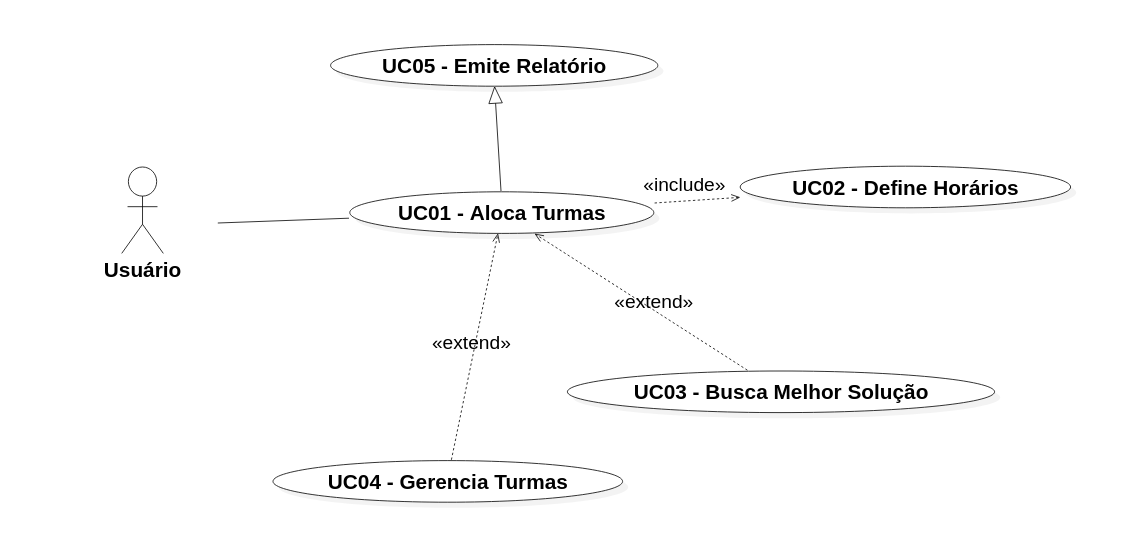
\includegraphics[width=1\textwidth]{TCC/imagens/casodeuso.png}
     \caption{Diagrama de Casos de Uso}
     \label{Diagrama de Casos de Uso}
\end{figure}

 
\subsubsection{Descrição dos Casos de Uso}


\begin{itemize}
    \item[] Descrição dos Atores
    
    \begin{itemize}
        \item[$\ast$] \textbf{Usuário}
        
        \textbf{Descrição} 
        
        Toda pessoa ou “software” que irá interagir com o sistema através de sua “interface” gráfica.
    \end{itemize}
    
    \item[] Casos de Uso
    
    \begin{itemize}
        \item[$\ast$] \textbf{$[$UC01$]$ -- Aloca Turmas}
        
        \textbf{Descrição}
        
         Este caso de uso permite que o usuário possa definir horários específicos de prova para alocar as turmas.
        
        \textbf{Pré-condições}
        \begin{enumerate}
            \item O usuário deve estar logado.
            \item O usuário deve ter turmas e seus respectivos alunos cadastrados no sistema.
            \item O usuário deve definir a quantidade de horários disponíveis para realização das provas.
        \end{enumerate}
       
        \textbf{Pós-condições}
        \begin{enumerate}
            \item  O sistema deve atribuir cada turma á um único horário.
            \item  O sistema deve informar a quantidade total de conflitos de alunos em duas turmas em um mesmo horário.
        \end{enumerate}
       
        
        \begin{table}[H]
            \centering
            \caption{Fluxo Principal de Interações de $[$UC01$]$}
            \vspace{0.5cm}
            \renewcommand\arraystretch{1.5}
            \begin{tabular}{c|p{6cm}|p{6cm}}
             
                \textbf{Sequência} & \textbf{Usuário} & \textbf{Sistema} \\ % Note a separação de col. e a quebra de linhas
                \hline                               % para uma linha horizontal
                1 & Seleciona uma turma e move para uma caixa de horário.  &  \\
                2 &   & Atribui a turma á um horário. \\
                3 & & Calcula o número de alunos que tenham duas provas em um mesmo de horário.          % não é preciso quebrar a última linha
                \\
                \hline
            \end{tabular}
        \end{table}
        
       
        
        \item[$\ast$] \textbf{$[$UC02$]$ -- Define Horários}
        
        \textbf{Descrição}
        
        Este caso de uso realiza a leitura da quantidade de horários de prova que o usuário dispõe para a realização das provas.
        
        \textbf{Pré-condições}
        \begin{enumerate}
            \item  O usuário deve estar logado. 
        \end{enumerate}
        
        \textbf{Pós-condições}
        \begin{enumerate}
            \item O sistema deve registrar como quantidade de horários um número maior ou igual a dois. 
            \item O sistema deve permitir a execução do caso de uso $[$UC01$]$.
        \end{enumerate}
        
     \begin{table}[H]
            \centering
            \caption{Sequência de Interações de $[$UC02$]$}
            \vspace{0.5cm}
            \renewcommand\arraystretch{1.5}
            \begin{tabular}{c|p{6cm}|p{6cm}}
             
                \textbf{Sequência} & \textbf{Usuário} & \textbf{Sistema} \\ % Note a separação de col. e a quebra de linhas
                \hline                               % para uma linha horizontal
                1 & Informa a quantidade de horários de prova disponível.  &  \\
                2 &   & Atualiza o número de caixas de horários.
                \\
                \hline
            \end{tabular}
        \end{table}
        
        \item[$\ast$] \textbf{$[$UC03$]$ -- Busca Melhor Solução}
        
        \textbf{Descrição}
        
        Este caso de uso permite ao sistema a executar um algoritmo de modo a buscar automaticamente uma alocação com o menor custo possível para as turmas selecionadas.
        
        \textbf{Pré-condições}
        \begin{enumerate}
            \item  O caso de uso $[$UC01$]$ deve ter sido executado.
            \item  O usuário precisa indicar todas as turmas que deverão realizar as provas nos horários indicados.
        \end{enumerate}
        
        \textbf{Pós-condições}
        \begin{enumerate}
            \item  O sistema deve encontrar a alocação que resulte no menor número de provas de segunda chamada forçadas pela alocação.
            \item O sistema deve encaminhar automaticamente o usuário para o caso de uso $[$UC05$]$.
        \end{enumerate}
        
        \begin{table}[H]
            \centering
            \caption{Fluxo Principal de Interações de $[$UC03$]$}
            \vspace{0.5cm}
            \renewcommand\arraystretch{1.5}
            \begin{tabular}{c|p{6cm}|p{6cm}}
             
                \textbf{Sequência} & \textbf{Usuário} & \textbf{Sistema} \\ % Note a separação de col. e a quebra de linhas
                \hline                               % para uma linha horizontal
                1 & Seleciona a opção de buscar a melhor solução.  &  \\
                2 &   & Executa algoritmo para buscar solução ideal. \\
                3 & & Redireciona para tela de Relatório com a solução ideal.          % não é preciso quebrar a última linha
                \\
                \hline
            \end{tabular}
        \end{table}
        
        \item[$\ast$] \textbf{$[$UC04$]$ -- Gerencia Turmas}
        
        \textbf{Descrição}
        
        Este caso de uso permite que o usuário crie, edite, remova, importe e exporte turmas, e seus respectivos alunos dentro do sistema.
        
        \textbf{Pré-condições}
        \begin{enumerate}
            \item  O usuário deve estar logado.
        \end{enumerate}
        
        \textbf{Pós-condições}
        \begin{enumerate}
            \item  O sistema deve atualizar o banco de dados com as novas informações assim que alteradas pelo usuário.
            \item  O sistema deve permitir alterações de forma simplificada pelo usuário.
            \item  O sistema deve exibir mensagens de alerta para o usuário em caso de alterações que não possam ser desfeitas.
        \end{enumerate}
        
       \begin{table}[H]
            \centering
            \caption{Fluxo de Interações de $[$UC04$]$ -- Criação de Turma}
            \vspace{0.5cm}
            \renewcommand\arraystretch{1.5}
            \begin{tabular}{c|p{6cm}|p{6cm}}
             
                \textbf{Sequência} & \textbf{Usuário} & \textbf{Sistema} \\ % Note a separação de col. e a quebra de linhas
                \hline                               % para uma linha horizontal
                1 & Seleciona a opção de “Adicionar Turma” na página de gerenciamento de turmas  &  \\
                2 &   & Redireciona a página atual para a página de “Criação de Turmas”  \\
                3 & Informa o nome da turma que deseja criar &    \\
                4 & Seleciona a opção para inserir o aluno & \\ 
                5 & & Cria a opção de inclusão de matrícula e nome para o novo aluno \\
                6 & Informa a matrícula e o nome do aluno & \\
                7 & Seleciona a opção “Criar Turma” & \\
                8 & & Grava turma no banco de dados \\ 
                9 & & Vincula alunos á turma criada \\
                10 & & Redireciona a página atual para a página de “Gerenciamento de Turmas"
                % não é preciso quebrar a última linha
                \\
                \hline
            \end{tabular}
        \end{table}
        
        \begin{table}[H]
            \centering
            \caption{Fluxo de Interações de $[$UC04$]$ -- Visualização de Turma}
            \vspace{0.5cm}
            \renewcommand\arraystretch{1.5}
            \begin{tabular}{c|p{6cm}|p{6cm}}
             
                \textbf{Sequência} & \textbf{Usuário} & \textbf{Sistema} \\ % Note a separação de col. e a quebra de linhas
                \hline                               % para uma linha horizontal
                1 & Seleciona a opção de “Visualizar” de uma turma  &  \\
                2 & & Redireciona a página atual para a página de “Visualização de Turma” \\
                3 & & Exibe uma lista em ordem alfabética com os alunos da turma         % não é preciso quebrar a última linha
                \\
                \hline
            \end{tabular}
        \end{table}
        
        \begin{table}[H]
            \centering
            \caption{Fluxo de Interações de $[$UC04$]$ -- Edição de Turma}
            \vspace{0.5cm}
            \renewcommand\arraystretch{1.5}
            \begin{tabular}{c|p{6cm}|p{6cm}}
             
                \textbf{Sequência} & \textbf{Usuário} & \textbf{Sistema} \\ % Note a separação de col. e a quebra de linhas
                \hline                               % para uma linha horizontal
                1 & Seleciona a opção de “Editar” uma turma  &  \\
                2 & & Redireciona a página atual para a página de “Edição de Turma” \\
                3 & & Exibe uma lista em ordem alfabética com os alunos da turma \\
                4 & & Habilita os campos de matrícula e nome para edição \\
                5 & Altera o nome e a matricula de um aluno & \\
                6 & Seleciona a opção “Salvar Alterações” & \\
                7 & & Atualiza a lista de alunos pertencentes á turma no banco de dados \\
                8 & & Redireciona a página atual para página de “Gerenciamento de Turmas” 
                % não é preciso quebrar a última linha
                \\
                \hline
            \end{tabular}
        \end{table}
        
        \begin{table}[H]
            \centering
            \caption{Fluxo de Interações de $[$UC04$]$ -- Exclusão de Turma}
            \vspace{0.5cm}
            \renewcommand\arraystretch{1.5}
            \begin{tabular}{c|p{6cm}|p{6cm}}
             
                \textbf{Sequência} & \textbf{Usuário} & \textbf{Sistema} \\ % Note a separação de col. e a quebra de linhas
                \hline                               % para uma linha horizontal
                1 & Seleciona a opção de “Apagar” uma turma  &  \\
                2 &   & Exibe um alerta \\
                3 & Seleciona a opção “Sim” no alerta &   \\
                4 & & Apaga a turma do banco de dados \\
                5 & & Atualiza a página de “Gerenciamento de Turmas"
                % não é preciso quebrar a última linha
                \\
                \hline
            \end{tabular}
        \end{table}
        
        \item[$\ast$] \textbf{$[$UC05$]$ -- Emite Relatório}
        
        \textbf{Descrição}
        
        Este caso de uso permite que o usuário visualize de forma gráfica os resultados e informações referentes a alocação feita, como a quantidade de alunos prejudicados pela alocação, e a lista de alunos que foram prejudicados.
        
        \textbf{Pré-condições}
        \begin{enumerate}
            \item  O caso de uso $[$UC01$]$ ou o caso de uso $[$UC02$]$ devem ter sido executados.
        \end{enumerate}
        
        \textbf{Pós-condições}
        \begin{enumerate}
            \item O sistema deve informar a quantidade de conflitos gerados pela alocação.
            \item O sistema deve informar os alunos prejudicados com duas provas alocadas em um mesmo horário.
            \item O sistema deve permitir o “download” e/ou impressão do relatório através de arquivo PDF.
        \end{enumerate}
        
       \begin{table}[H]
            \centering
            \caption{Fluxo Principal de Interações de $[$UC05$]$}
            \vspace{0.5cm}
            \renewcommand\arraystretch{1.5}
            \begin{tabular}{c|p{6cm}|p{6cm}}
             
                \textbf{Sequência} & \textbf{Usuário} & \textbf{Sistema} \\ % Note a separação de col. e a quebra de linhas
                \hline                               % para uma linha horizontal
                1 & Conclui a alocação das turmas em seus respectivos horários para realizarem as provas.  &  \\
                2 &   & Exibe a quantidade de provas de segunda chamada necessárias com a alocação.       \\
                3 & & Exibe a alocação feita.     \\
                4 & & Fornece a opção de gerar PDF do relatório. \\ 
                5 & & Fornece a opção de realizar nova alocação. % não é preciso quebrar a última linha
                \\
                \hline
            \end{tabular}
        \end{table}
        
    \end{itemize}
    
\end{itemize}




\subsection{Diagrama de Atividades}
 
 O diagrama de atividades auxilia na criação e representação de um fluxo de utilização de um sistema por um usuário.
 
 O diagrama \ref{Diagrama Atividades} apresenta o comportamento do sistema a medida em que um usuário acessa suas funcionalidades, iniciando em sua  primeira conexão ao sistema até a impressão do relatório contendo o resultado obtido com a alocação realizada.
 
 \begin{citacao}
     Os diagramas de atividades são uma técnica para descrever lógica de procedimento, processo de negócio e fluxo de trabalho. De várias formas, eles desempenham um papel semelhante aos fluxogramas, mas a principal diferença entre eles e a notação de fluxograma é que os diagramas suportam comportamento paralelo. \cite[p. 118]{fowler07}
 \end{citacao}
 
\begin{figure}[H]
     \centering
     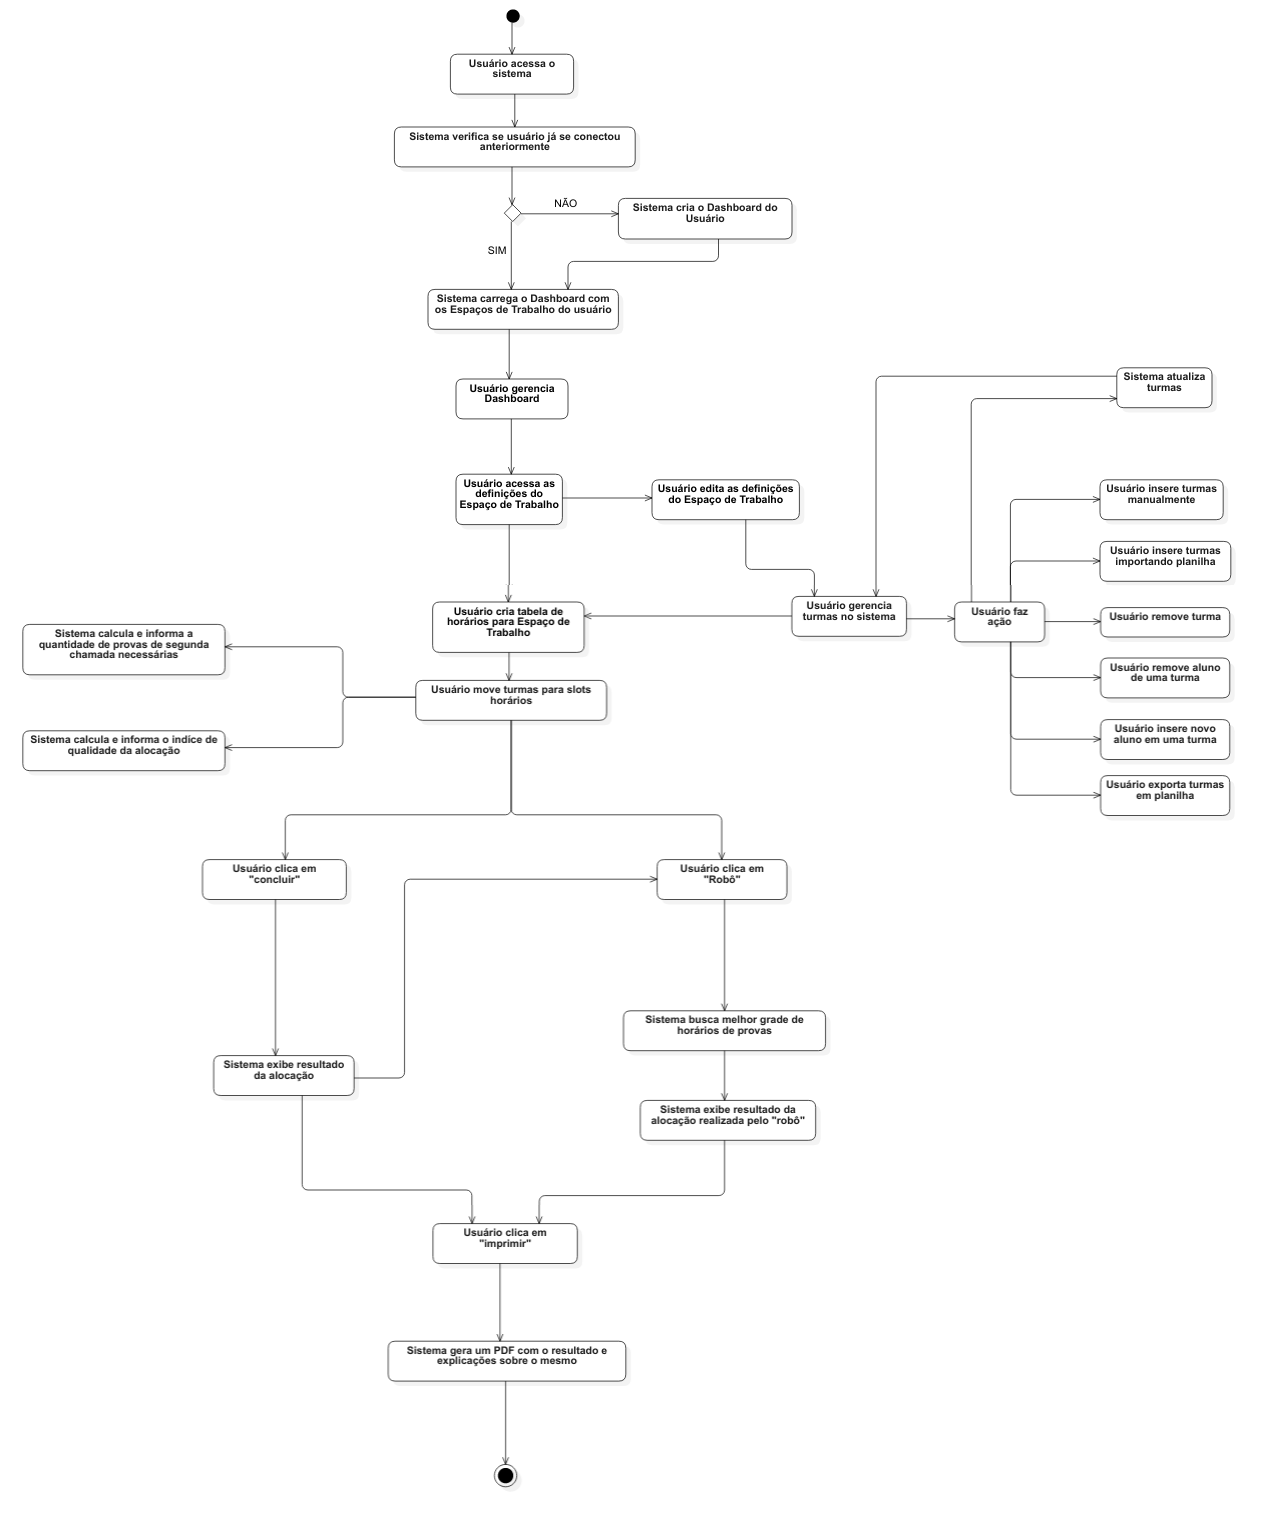
\includegraphics[width=1.1\textwidth]{TCC/imagens/atividades.png}
     \caption{Diagrama de Atividades}
     \label{Diagrama Atividades}
\end{figure}

 
 
\subsection{Diagrama de Classes}

O diagrama de classes é um dos diagramas mais utilizados em UML, ele apresenta a forma pela qual o código está estruturado, permitindo dessa forma, que outros desenvolvedores possam compreender o funcionamento do “software”, facilitando dessa maneira a organização do código e sua manutenção ao longo do tempo.

% O diagrama apresentado em \ref{Diagrama de Classes} consiste na utilização das classes \emph{usuário}, que será responsável por interagir com o sistema, \emph{espaço de trabalho}, qe poderá representar tanto uma instituição quanto um grupo de turmas, \emph{turmas}, e seus respectivos \emph{alunos}, e a \emph{grade de provas} que consiste no controle do resultado e a alocação.

 \begin{citacao}
      Um diagrama de classes descreve os objetos presentes no sistema e os vários relacionamentos estáticos existentes entre eles. Os diagramas de classes também mostram as propriedades e as operações de uma classe e as restrições que se aplicam à maneira como os objetos estão conectados. A UML utiliza a palavra característica como um termo geral que cobre as propriedades e operações de uma classe. \cite[p. 52]{fowler07}
 \end{citacao}
 
\begin{figure}[H]
     \centering
     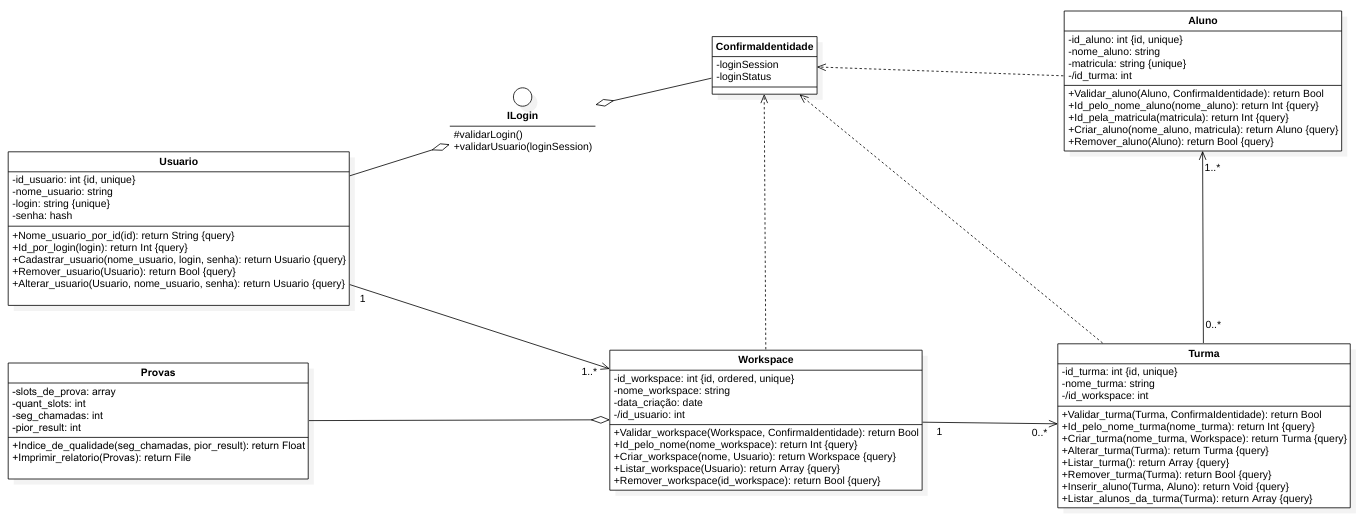
\includegraphics[width=1.4\textwidth,angle=270]{TCC/imagens/classes.png}
     \caption{Diagrama de Classes}
     \label{Diagrama de Classes}
\end{figure}


\subsection{Diagrama de Entidade-Relacionamento}

O diagrama de entidade-relacionamento é utilizado para permitir a representação geométrica das relações entre diferentes entendidas abstratas, podendo essas serem pessoas, cargos, objetos, imóveis e quaisquer outros conjuntos que possuam atributos em comum que os permita serem diferenciados.

O diagrama neste trabalho apresenta as relações entre turmas e seus respectivos alunos, as turmas que compõem um espaço de trabalho (\textit{workspace}), que representarão um conjunto de turmas,  por exemplo uma instituição ou turno, e dessa forma a relação entre um usuário e todos os seus espaços de trabalho.

  \begin{citacao}
   A técnica de modelagem de dados mais difundida e utilizada é a abordagem entidade-relacionamento (ER). Nesta técnica, o modelo de dados é representado através de um modelo entidade-relacionamento (ER). Usualmente, um modelo ER é representado graficamente, através de um diagrama entidade-relacionamento (DER). A abordagem ER foi criada em 1976 por Peter Chen. Ela pode ser considerada um padrão de fato para modelagem conceitual. \cite[p. 12]{heuser09}
    \end{citacao}
    
\begin{figure}[!h]
     \centering
     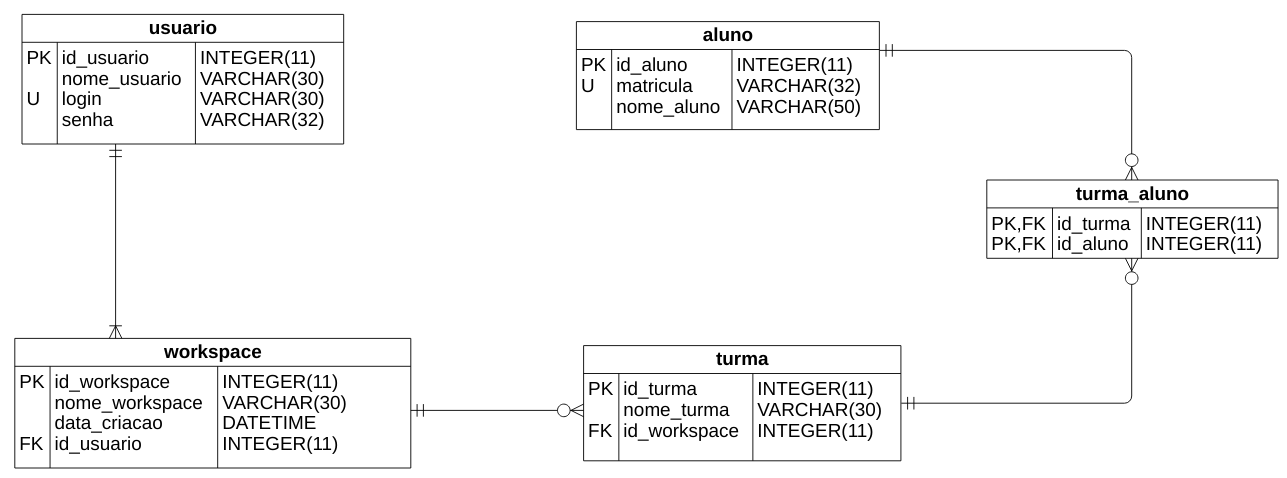
\includegraphics[width=1\textwidth,angle=270]{TCC/imagens/DER.png}
     \caption{Diagrama de Entidade Relacionamento}
     \label{Diagrama de Entidade Relacionamento}
\end{figure}
 
% \subsection{Diagrama de Fluxo de Telas}

\subsection{Relatórios}

O relatório gerado pelo sistema tem como propósito ser um documento para o usuário com as informações referentes a forma como as turmas foram distribuídas, possíveis conflitos causados pela alocação, e explicações sobre a construção e funcionamento do sistema.

Seu foco é: ser instrutivo, de modo a permitir que o usuário consiga replicar o resultado em uma universidade real. Ser didático, visando explicar as bases do problema matemático por trás do problema de horários de exames universitários e a proposta de solução usada no trabalho.

A partir do arquivo PDF gerado pelo sistema, é possível efetuar o “download” do relatório e salva-lo digitalmente, e também permite a impressão do mesmo, caso seja desejável ter uma versão física da solução.

Dessa forma o relatório serve tanto como uma instrução de como a grade de prova poderá ser realizada, como um documento com propósito explicativo que justifique a alocação e que antecipe os problemas que por ventura venham a acontecer, no caso os alunos com mais de uma prova em um mesmo horário.
	
	

    % \include{capitulos/algoritmo}

	% \include{capitulos/resultados}



	 \phantompart								%
	% --------------------------------------------------------------------
	% Insira abaixo o capitulo de Conclusão do Trabalho
	%
	% --------------------------------------------------------------------


	%\part{Considerações Finais}
    \chapter{Resultados Obtidos e Trabalhos Futuros}
\label{cap:resultados}

% \section{Conclusão da Pesquisa Realizada}
Este trabalho visou obter o melhor resultado possível considerando as turmas, seus alunos e a quantidade de horários disponíveis na instituição para realização das provas. Dessa forma foi apresentado tanto conceitualmente quanto de forma prática, nos resultados da aplicação proposta, a melhor alocação e suas possíveis consequências. Permitindo dessa forma, que ajustes por parte do usuário sejam realizadas sobre as provas de segunda chamada naquele cenário em específico.

Apresentamos formalmente neste trabalho o problema de programação de horários de exames universitários com suas respectivas classificações e restrições, demonstramos também a modelagem matemática para o problema e propomos um algoritmo capaz de obter uma solução adequada para as condições estabelecidas, além de ofertar essa solução na forma de um sistema que permite a busca pela resolução de forma automática e amigável para qualquer usuário.

% Foi utilizada a estrutura matemática da Teoria dos Grafos para modelar o problema, mais especificamente de Grafos de Interseção e Coloração de Vértices. Este modelo nos permitiu a utilização de um enorme acervo de pesquisas e publicações sobre o tema. 

Com o desenvolvimento de uma solução computacional, foi possível automatizar o processo de busca por soluções, facilitando o trabalho das pessoas e principalmente, permitindo-as obter uma melhor solução com uma expressiva redução no tempo de busca, em comparação com métodos manuais. 

Visando o desenvolvimento de um produto amigável para o usuário final (\emph{user-friendly}), foi um objetivo desse trabalho tornar transparente a utilização de abstrações, estruturas e modelos matemáticos, atendendo aos fundamentos de simplicidade, compatibilidade, navegabilidade e reusabilidade a fim de permitir o emprego futuro deste trabalho em pesquisas de natureza similar.

%  \section{Metodologia Cientifica Utilizada}

% \begin{enumerate}
%    \item Finalidade - Pesquisa Aplicada
%    \item Objetivos - Descritiva
%    \item Abordagem - Quantitativo
%    \item Método - Hipotético-dedutivo
%    \item Procedimentos - Bibliográfico, Experimental e Estudo de Caso
% \end{enumerate}

Em nossa pesquisa utilizamos a abordagem quantitativa, onde realizaríamos um teste de usabilidade a fim de validar nosso protótipo desenvolvido. Usaríamos como instrumento de coleta de dados um questionário, com 25 perguntas. Na elaboração das perguntas, procuramos investigar o conhecimento dos usuários sobre sua área de atuação profissional, a fim de detectar possíveis usuários finais, o conhecimento prévio do usuário sobre o tema, sua facilidade em identificar as funcionalidades do sistema e sua consequente utilização.

O instrumento não foi aplicado aos usuários na forma de um teste de usabilidade no ano de 2020, devido a limitações causadas devido as restrições distanciamento social impostas em meio a pandemia de Covid-19 causada pelo vírus Sars-Cov2, popularmente conhecido como Coronavírus.  Os usuário responderiam ao questionário em forma de entrevista enquanto realizariam o teste do sistema de forma guiada, na qual deveriam seguir instruções recebidas durante a utilização do sistema.

Contudo, o roteiro desenvolvido para a aplicação dos testes de usabilidade está disponível em apênce do trabalho e poderá ser aplicado juntamente as adequações observadas em \textbf{Trabalhos Futuros}.
% Através dos procedimentos de análise dos dados, chegamos aos gráficos apresentados a seguir, onde podemos observar as respostas mais comuns para as perguntas realizadas e identificar assim os problemas mais relatados e a percepção do uso da aplicação por usuários comuns.

% \section{Resultados dos Testes de Interface}




 \section{Trabalhos Futuros}

% ---

Segundo pesquisa realizada pelo \citeonline{ceticbr19}, 99\% da população brasileira que possuía acesso à “internet” tinha um aparelho celular em 2019, sendo que, para 58\% da população com acesso à “internet”, o aparelho celular era o único meio para se conectar a rede. Considerando informações desse gênero, fica evidente à necessidade de se criar futuramente adequações no protótipo visando atingir um público mais amplo.

Para que seja possível deixar o protótipo totalmente funcional em “smartphones”, será necessário realizar algumas adaptações na “interface” da aplicação, aumentando sua responsividade e adicionando mais ações para os eventos disparados ao pressionar sobre a tela do dispositivo, que são diferentes dos \emph{cliques} com o cursor do mouse. Dessa forma, tornar o protótipo inicial em um produto multiplataforma, sem perder seu propósito e funcionamento.

Visando obter um melhor desempenho, é interessante a realização de uma pesquisa para implementar outros métodos Heurísticos propostos na literatura, tanto para o problema de programação de horários de exames universitários, quanto expandi-los para problemas de escalonamento de horários de aulas com devidas adaptações. Dessa forma pretendemos comparar os diferentes resultados e desempenhos obtidos com cada proposta, visando ao final, utilizar desse conhecimento para, quem sabe, propor uma nova heurística específica que resolva o problema apresentado neste trabalho.

 Após a criação e implementação dessa heurística pretendemos a comparar seus resultados com demais heurísticas, caso ela se demonstre promissora, será um desejo utilizar instâncias de dados realistas para realizar testes. Para isso uma base de dados postulante seriam os dados do \emph{International Competition Timetabling} ou ICT, que se trata de uma competição internacional para avalizar algoritmos heurísticos (em grande parte) no processo de resolução do problema clássico de \emph{Timetabling}, que é alocar professores, turmas e salas em horários específicos dadas uma série de restrições utilizando uma base real de dados de uma determinada instituição universitária.

Apesar de o problema estudado no trabalho e o problema de alocação de professores em salas de aula, juntamente as suas turmas e horários serem similares em natureza, será necessário alterar sutilmente algumas informações, e acrescentar uma informação a base de dados, será necessário inicialmente retirar da modelagem os professores e suas restrições, as salas de aula e suas restrições, entre outras, e incluir o número máximo de horários de prova que aquele conjunto de turmas poderá fazer, para dessa forma ser possível utilizar uma base de dados real para submeter as heurísticas a testes e de acordo com seus resultados, buscar aplicá-las em problemas parecidos.


 
	 \chapter{Considerações Finais}
\label{cap:conclusao}
% ---

% \section{Problema Geral}  \section{Problema Específico}

% JUSTIFICATIVA + TEMA
Ao produzir um sistema amigável utilizando a coloração de grafos de interseção para resolver o problema de programação de horário de exames em universidades, obtivemos exito em facilitar a obtenção do resultado de uma forma simplificada e organizada.

% \section{Objetivos Gerais}
O trabalho trouxe uma abordagem em que se obteve o melhor resultado possível considerando as turmas, seus alunos e a quantidade de horários de provas disponíveis na instituição. Sendo apresentado conceitualmente e de forma prática na aplicação proposta, a melhor alocação e suas possíveis consequências, permitindo dessa forma, que fossem realizadas as aplicações das provas de segunda chamada da melhor forma possível.

% \section{Objetivos Específicos}

Mesmo possuindo vasta quantidade e qualidade de referências e propostas de algoritmos eficientes que objetivassem solucionar o problema, não foi observado em nenhuma das pesquisas citadas uma aplicação voltada para o usuário final, considerando a possibilidade da utilização do “software” por um leigo em matemática ou computação.

No decorrer do trabalho, foi apresentado formalmente o problema de programação de horários de exames universitários com suas respectivas classificações e restrições, demonstrada a modelagem matemática para o problema e propondo um algoritmo capaz de obter o melhor resultado, além de apresentado um sistema que permite a realização da busca pela resolução de forma automática, contudo se mantendo amigável para qualquer usuário.

% \section{Hipótese / Estratégia}

A documentação do processo, partindo da identificação de um problema de natureza combinatória até o desenvolvimento de um produto amigável para um usuário final, por meio da utilização de abstrações, estruturas e modelos matemáticos, não é comum em trabalhos de conclusão de curso da instituição, contudo, visando uma maior disseminação dessas informações no âmbito da instituição e possibilitar a (re)utilização futura de partes deste trabalho em pesquisas de problemas de natureza similar, optamos seguir por este caminho.

% \section{Organização do Trabalho}

Buscando desenvolver um “software” fosse capaz de resolver o problema, mantendo sua simplicidade e sendo intuitivo ao máximo para os usuários finais, foi necessário que o problema estivesse bem estruturado, possibilitando a solução encontrada por meio da aplicação fosse completamente satisfatória tanto do ponto de vista de usabilidade, quanto do ponto de vista conceitual e matemático.

% RESULTADOS OBTIDOS

\section{Limitações da Pesquisa}

No decorrer da pesquisa, uma série de referências foram consultadas a fim de fundamentar de forma expressiva os métodos, ferramentas e expressões usadas no trabalho. No entanto devido ao excedente de informações relativas a diversos pontos, fez-se necessário que o trabalho adotasse uma postura mais didática e por vezes superficial sobre alguns temas.

Devido a opção de se realizar um trabalho mais didático e prático, considerando ser uma pesquisa de graduação tecnóloga de Análise de Sistemas, a parte matemática do trabalho carece de maiores detalhes e aprofundamento. Contudo as referências citadas ao longo do trabalho possuem pesquisas com grande enfoque matemático, sendo de certa forma complementar ao apresentado.

A modelagem UML do sistema carece de uma documentação mais extensa ao se comparar com as recomendações de autores do tema, contudo a escolha por realizar uma documentação mais simples foca-se na flexibilização para possibilitar a reutilização da modelagem em futuras implementações. Contudo a opção deixa a documentação mais distante do sistema a ser desenvolvido de fato.

Na parte da análise dos resultados obtidos e observados com a utilização do protótipo através do teste de usabilidade não foi realizado, devido as restrições impostas pelo distanciamento social causado pela pandemia de Covid-19 causada pelo vírus Sars-Cov2, popularmente conhecido como Coronavírus, contudo o registro do questionário e roteiro permitirá a aplicação do experimento e a consequente validação do protótipo em oportunidades futuras.


\section{Recomendações para Pesquisas Futuras}

Os problemas de programação de horários são vastos na literatura e permitem a resolução de problemas de naturezas diferentes, assim como os problemas similares citados, de alocação de bandas em dias de um festival, escalas de equipes em uma companhia aérea e a distribuição de recursos militares. Existem ainda muitos outros problemas não enunciados que podem ser modelados da mesma forma e por fim serem solucionados pelos mesmos métodos.

Estudos de problemas similares podem focar tanto em explorar as abordagens da solução do modelo matemático, através de métodos determinísticos ou não-determinísticos, ou na criação de sistemas personalizados voltados para resolução de uma determinada demanda.

Trabalhos nas áreas da Teoria dos Grafos e de resolução de problemas de natureza combinatória por muitas vezes focam-se apenas na modelagem e solução matemática ou algorítmica do modelo, e muitas vezes não produz um sistema voltado para um usuário real, é recomendada a implementação de sistemas que apliquem essas as soluções, hoje abstratas, para muitos problemas.

Observa-se também que existe a possibilidade de se expandir as variáveis consideradas no problema, de forma que sejam ponderadas questões como quantidade máxima de alunos a realizarem provas em um mesmo horário, quantidade de salas disponíveis simultaneamente para realização dos exames, quantidade de professores ou aplicadores disponíveis em cada horário, minimização da quantidade de provas de segunda chamada para um mesmo aluno, entre muitos outros que poderiam ser inclusos.

Ao se prosseguir com pesquisas e desenvolvimento, no âmbito principalmente da graduação, de ferramentas voltadas para temas similares ao apresentado nesse trabalho, cada vez mais serão populares os métodos de modelagem e resolução de problemas de natureza combinatória, que estão entre os mais complexos da computação e talvez os que resolvam o maior número de problemas cotidianos considerados complicados. Também será aumentada a quantidade de aplicações automatizadas para problemas cotidianos, beneficiando dessa forma toda a sociedade, além proporcionar aumento considerável do acervo de conhecimento científico em língua portuguesa sobre esses problemas.
 
   

 	\postextual									%
 	% --------------------------------------------------------------------
 	% Insira abaixo os capítulos pós-textuais do seu trabalho
 	% como: bibliografia, apêndices e anexos
 	% --------------------------------------------------------------------
    
 	% para inserir bibtex -> \bibliography{localdoarquivo/nomedoarquivo} (não coloque extensão)
    
    \nocite{poulsen13,rocha13,gotlieb63,wren96,schaerf99,santos07,poulsen12,burke95a,garey79,dwerra95,ross95,burke95b,cormen14,page-jones01,larman00,fowler07,sommerville11,pressman11,szwarcfiter94,szwarcifter86,sedgewick,feofiloff11,yoshiko12,vredeveld_02,goldbarg_12,goldbarg_15,heuser09}
   
   \nocite{bezerra2007principios, biajolinovas, borges2003resoluccao, brucker2007, burke2010decomposition, burke2002recent, burke2007practice, cacchiani2013tutorial, cerioli2012minicurso, richard1967theory, cormen2001, csima1964, da2010heuristicas, daalgoritmo, diverio2009teoria, eiselt2013decision, elmaghraby2012symposium, feofiloff2011minicurso, klein1994algoritmos, knuth1997stable, kostuch2004hardness, levitin2012introduction, martin2019codigo, menezes2017formulaccoes, sipser2007introduccao, monteiro2017heuristicas, muhlenthaler2015fairness, neufeld1974graph, oliveira2011timetabling, pereira2017inserccao, pinedo2005planning, pinedo2012scheduling, reis2006introduccao, rodrigues2008tratamento, schmidt1980timetable, werner2018special}
	\bibliography{referencias/referencias}
 	
 	 % ---------------------------------------------------------
	% Apêndices
	% ---------------------------------------------------------
 	
 	\begin{apendicesenv}

% Imprime uma página indicando o início dos apêndices
\partapendices

% ----------------------------------------------------------
\chapter{Roteiro}
\label{cap:roteiro}
A seguir está o roteiro para realização do teste de usabilidade do sistema desenvolvido, e de forma conjunta as perguntas referentes ao questionário de percepção do usuário.

\begin{enumerate}
    \item[I --] \textbf{Apresentação}

Agradeço a participação no teste de usabilidade do protótipo do sistema de agendamento de provas.

    \item[II --] \textbf{Identificação do Usuário}

Antes de iniciarmos é necessário informar os seguintes dados:

\begin{itemize}
    \item Qual seu nome?
    \item Qual seu “e-mail”?
    \item Qual profissão ou ocupação?
    \item Já utilizou ou viu esse sistema anteriormente?
    \item Conhece o trabalho ao qual o sistema pertence?
\end{itemize} 

Esses dados serão utilizados para permitir quantificar sua experiência com a usabilidade do sistema.

    \item[III --] \textbf{Identificação do Sistema}
   
Você estará sendo orientado(a), conforme as ação você deverá tomar ao utilizar o sistema, e simultaneamente serão realizadas perguntas sobre sua experiência. 
 
\begin{citacao}
    Neste momento do teste o usuário deverá ser conduzido até á página onde se encontra o sistema, e deverá ser realizado login utilizando um usuário predefinido que só é possuidor do espaço de trabalho padrão: “exemplo”.
\end{citacao}

Observe a página atual do sistema por 15 segundos e responda:

\begin{itemize}
    \item Qual a finalidade dessa página para você? 
    \item Você consegue dizer quais os recursos estão disponíveis nessa página?
\end{itemize}

Agora identifique onde está o menu principal do sistema e visualize suas informações.

Agora crie um novo \textbf{Espaço de Trabalho} com o título “Minha Escola”.

Acesse o \textbf{Espaço de Trabalho} “Minha Escola”.

Retorne até a página “\textbf{Dashboard}”, por favor.

Apague o \textbf{Espaço de Trabalho} “Minha Escola”. 

Responda a seguir:

\begin{itemize}
    \item Você teve alguma dificuldade em seguir alguma instrução?
\end{itemize}

    \item[IV --] \textbf{Espaço de Trabalho}

Acesse as \textbf{Definições} do \textbf{Espaço de Trabalho} “exemplo”.

Observe por 15 segundos esta página e responda a seguir.

\begin{itemize}
    \item Qual a finalidade dessa página para você? 
    \item Você consegue dizer quais os recursos estão disponíveis nessa página?
\end{itemize}

    \item[V --] \textbf{Gerenciamento das Turmas}
    
Acesse a página para \textbf{Gerenciar as Turmas} do “exemplo”.

Observe a página por 15 segundos e responda:

\begin{itemize}
    \item Qual a finalidade dessa página para você? 
    \item Você consegue dizer quais os recursos estão disponíveis nessa página?
\end{itemize}

Visualize os alunos de alguma das turmas.

Insira um novo aluno na turma.

Remova esse aluno da turma.

Retorne as \textbf{Definições} do \textbf{Espaço de Trabalho} “exemplo”.

\begin{itemize}
    \item Você teve alguma dificuldade em seguir alguma instrução até esse momento?
\end{itemize}
    
    \item[VI --] \textbf{Criar Tabela de Horários}

Crie uma \textbf{Tabela de Horário} para “exemplo”.

Visualize as opções no menu secundário da página.

Observe a página por 15 segundos e responda a seguir:

\begin{itemize}
    \item Qual a finalidade dessa página para você? 
    \item Você consegue dizer quais os recursos estão disponíveis nessa página?
\end{itemize}

Aumente a quantidade de horários de prova.

Defina o horário em que a primeira turma deverá realizar prova.

Defina o horário para as demais turmas de “exemplo” realizarem prova.

Observe a página por 10 segundos e responda a seguir:

\begin{itemize}
    \item Você consegue dizer quais os recursos estão disponíveis nessa página?
\end{itemize}

Gere um \textbf{Relatório} com os horários de prova que você determinou.

    \item[VII --] \textbf{Relatório}

Observe a página por 15 segundos e responda a seguir:

\begin{itemize}
    \item Qual a finalidade dessa página para você? 
    \item Você consegue dizer quais os recursos estão disponíveis nessa página?
\end{itemize}

Visualize os alunos que deverão realizar duas provas diferentes em um mesmo horário.

Utilize o \textbf{Robô} para encontrar uma nova tabela de horários de prova.

    \item[VIII --] \textbf{Robô}
    
Observe a página por 15 segundos e responda a seguir:

\begin{itemize}
    \item Existe alguma diferença para a página anterior? 
\end{itemize}

Salve o relatório do resultado como um \textbf{PDF}.

    \item[IX --] \textbf{Avaliação Geral}
    
Responda as perguntas a seguir para finalizar o teste.

\begin{itemize}
    \item Você utilizaria esse sistema para gerar grades de horários de prova?
    \item Entre 1 e 5, qual seria sua avaliação sobre sua utilização do sistema?
    \item Você recomendaria esse sistema para uma pessoa que precisasse criar grades de horários de prova?
    \item Você conhece ou já utilizou algum sistema similar a esse?
    \item Se você precisasse definir o sistema em uma palavra, qual seria?
\end{itemize}

Muito obrigado por participar deste teste de usabilidade.

\end{enumerate}

\end{apendicesenv}
 	
    % ---------------------------------------------------------
	% Anexos
	% ---------------------------------------------------------

 	% \include{capitulos/anexo}
      
\begin{anexosenv}
\partanexos
\chapter{Prot\'otipo}
\pagestyle{simple}
\label{cap:manual}

\section{Instalação}

\subsection{Pré-requisitos do Projeto}

Programas necessários para realizar a utilização do \textit{software}:

\begin{itemize}
    \item \textbf{Apache Server}.
    \item \textbf{PHP} \textit{7.0 ou superior}.
    \item \textbf{MariaDB} \textit{10 ou superior}.
    \item \textbf{GIT}.
\end{itemize}

Após verificar a existência dos programas citados e suas respectivas versões, pode ser iniciado o processo de instalação.

Para realizar a instalação deve-se entrar no diretório indicado pelo servidor \textbf{Apache} no seu sistema operacional através terminal (ou \textit{console}), e após isso executar os comandos de acordo com o tutorial contido no repositório do protótipo  \url{http://github.com/FilipeRodrigues3003/TCC/agendador}. Com isso você irá copiar os arquivos do protótipo para o diretório do seu servidor local.


\section{Utilização}

Após a instalação pode-se acessar o software a partir de \url{//localhost/agendador} para acessar o protótipo em caso de instalação seu próprio computador, ou através de \url{http://ipdoseuservidor/agendador} caso tenha feito a instalação em um servidor remoto.

Ao acessar pela primeira vez será exibida a página de \textit{\textbf{Login}} conforme figura \ref{tela-login} abaixo, caso o usuário ainda não possua um \textit{login}, este deverá clicar sobre o botão \textbf{Cadastre-se}.

%% Tela Login
\begin{figure}[H]
     \centering
     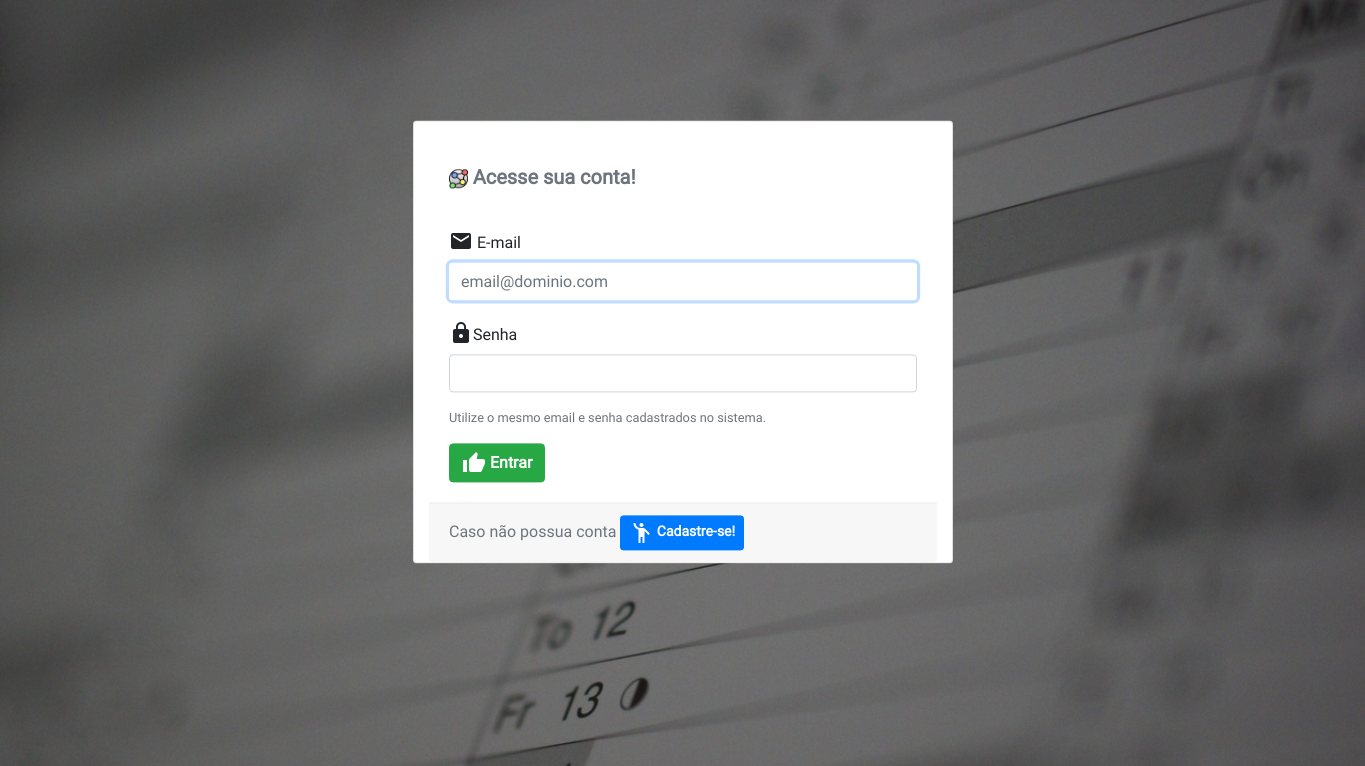
\includegraphics[width=0.8\textwidth]{TCC/imagens/sistema/01.png}
     \caption{Tela de Login}
     \label{tela-login}
\end{figure}

\subsection{Cadastro de Usuários}

Para que seja possível utilizar o sistema, é necessário que o usuário possua um \textit{login} no mesmo, e para isso o usuário deverá realizar um pequeno cadastro na página apresentada na figura \ref{tela-cadastro-usuario}. 

O usuário deverá informar obrigatoriamente: seu nome completo, endereço de \textit{e-mail} válido e uma senha.

%% Tela Cadastro de Usuário
\begin{figure}[H]
     \centering
     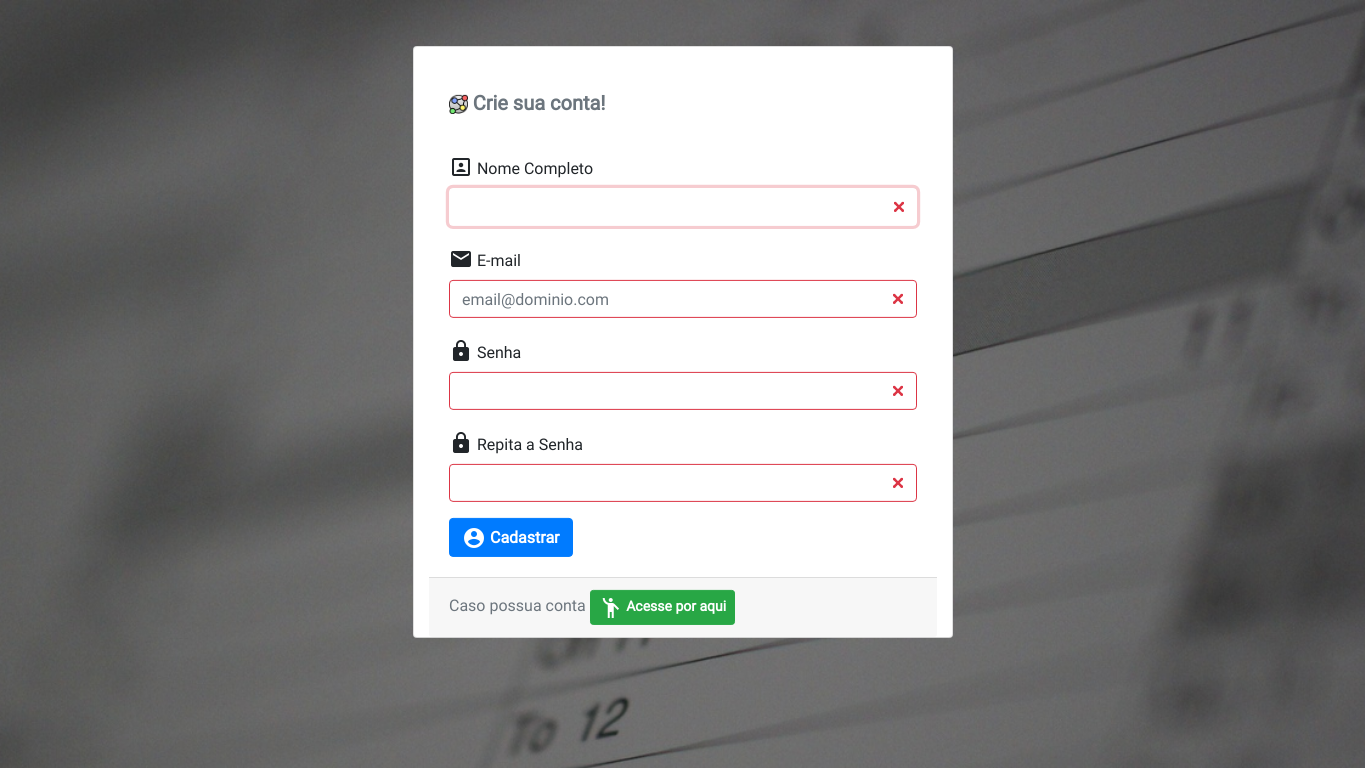
\includegraphics[width=0.8\textwidth]{TCC/imagens/sistema/02.png}
     \caption{Tela de Cadastro de Usuário}
     \label{tela-cadastro-usuario}
\end{figure}

A partir do momento em que o usuário realizar seu cadastro, será possível efetuar \textit{login} no sistema. Para isso o usuário deverá submeter seu \textit{e-mail} e senha (conforme informado no cadastro).


\subsection{Dashboard}

Após efetuar o \textit{login}, o usuário estará na tela de \textbf{Dashboard} do sistema, na qual visualizará seus \textbf{espaços de trabalho}, o \textbf{menu de navegação principal}, no topo da página, além da opção de \textbf{criar novos espaços de trabalho}.

%% Tela de Dashboard
\begin{figure}[H]
     \centering
     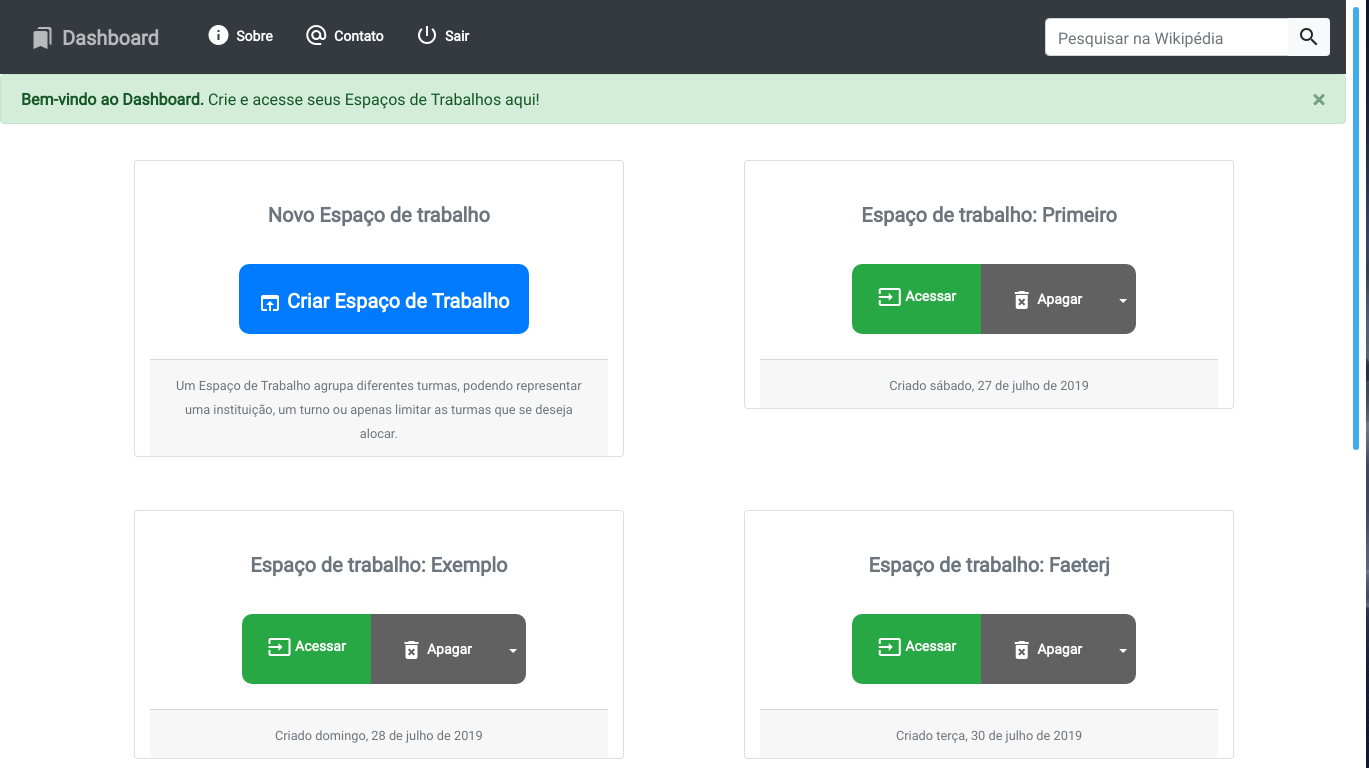
\includegraphics[width=0.8\textwidth]{TCC/imagens/sistema/03.png}
     \caption{Tela de Dashboard}
     \label{tela-dashboard}
\end{figure}

Um \textbf{espaço de trabalho} aqui é análogo a uma instituição, turno ou qualquer outra forma pela qual o usuário deseja separar as turmas que deverão ter as grades de prova geradas.

Para se \textbf{criar um novo espaço de trabalho} deve-se clicar no botão azul escrito "Criar Espaço de Trabalho"\ no \textit{\textbf{Dashboard}}, e informar o nome que o espaço de trabalho deverá ter, como mostrado na figura \ref{tela-new-workspace}.
%% Tela Login
\begin{figure}[H]
     \centering
     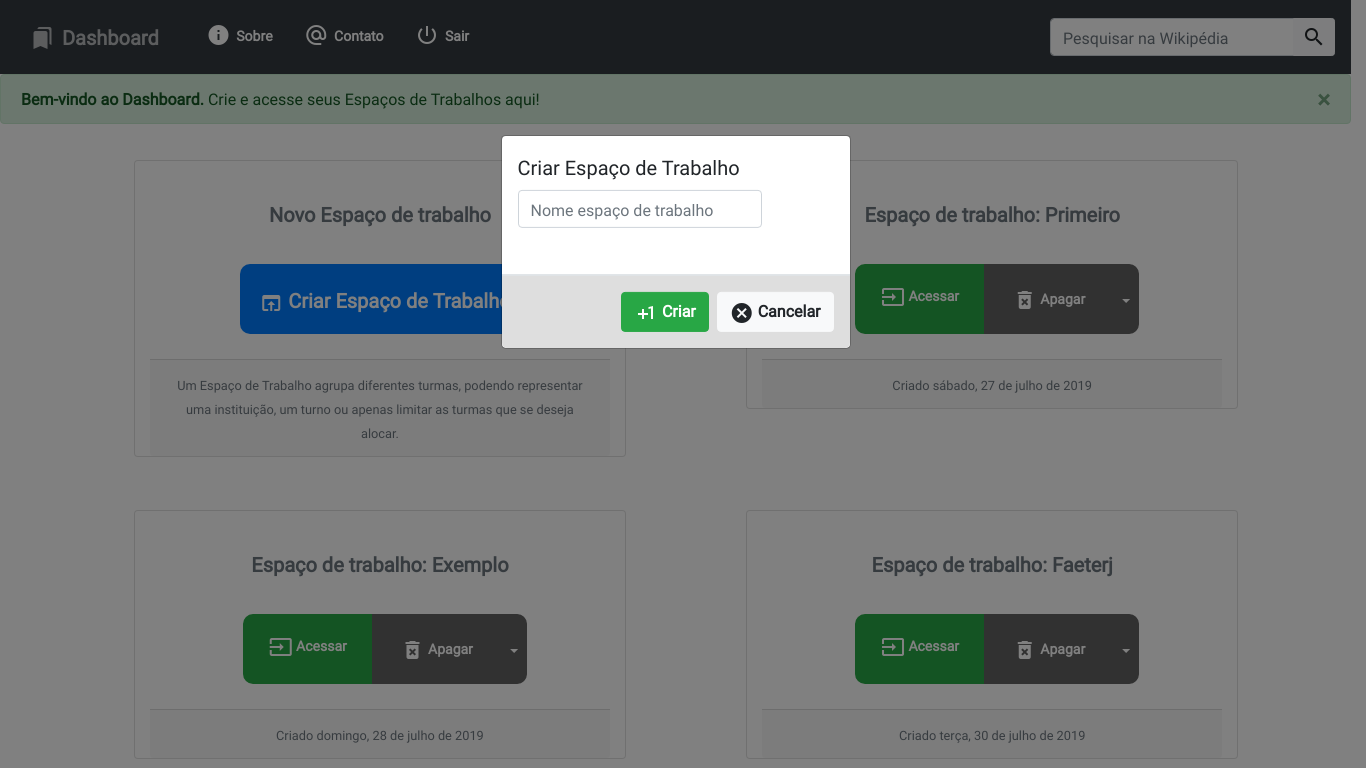
\includegraphics[width=0.8\textwidth]{TCC/imagens/sistema/03b.png}
     \caption{Tela de Criação de Novo Espaço de Trabalho}
     \label{tela-new-workspace}
\end{figure}

No canto direito do \textbf{menu de navegação principal} temos uma barra de pesquisa, que serve para auxiliar o usuário em caso de dúvidas com termos técnicos, fazendo consultas diretamente na enciclopédia online \url{Wikepédia.org} observado na figura \ref{tela-wiki}, possibilitando dessa forma esclarecer as dúvidas sem ser necessário deixar a tela do sistema como apresentado na figura \ref{tela-popup}.
%% Tela Login
\begin{figure}[H]
     \centering
     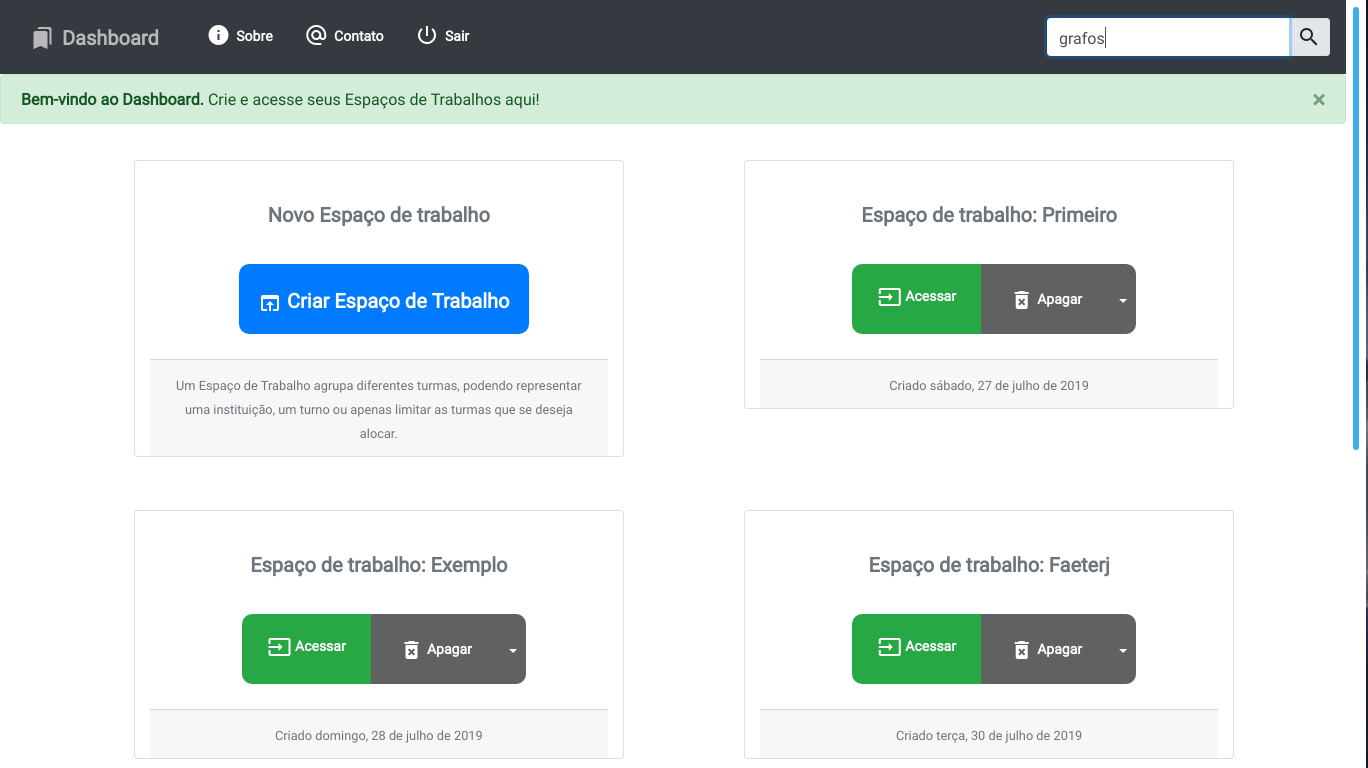
\includegraphics[width=0.8\textwidth]{TCC/imagens/sistema/03c.png}
     \caption{Tela de Campo de Busca na Wikipédia}
     \label{tela-wiki}
\end{figure}

%% Tela Login
\begin{figure}[H]
     \centering
     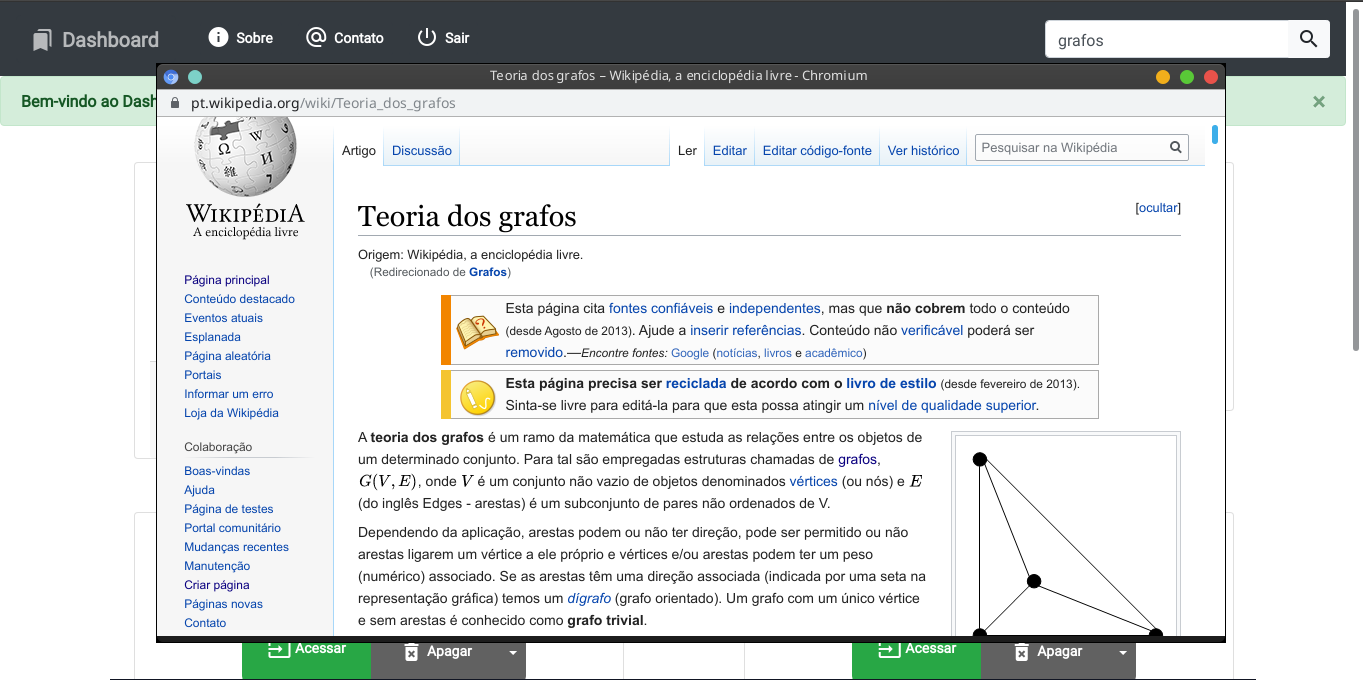
\includegraphics[width=0.8\textwidth]{TCC/imagens/sistema/03d.png}
     \caption{Tela de Campo de Busca na Wikipédia Pop-up}
     \label{tela-popup}
\end{figure}

Ainda no \textbf{menu de navegação principal}, da esquerda para direita observamos as seguintes opções:

Em \textbf{Sobre} que apresentará informações sobre o sistema, como o autor, os objetivos do projeto e como foi realizado o desenvolvimento do protótipo, assim como vemos na figura \ref{tela-sobre}
%% Tela Login
\begin{figure}[H]
     \centering
     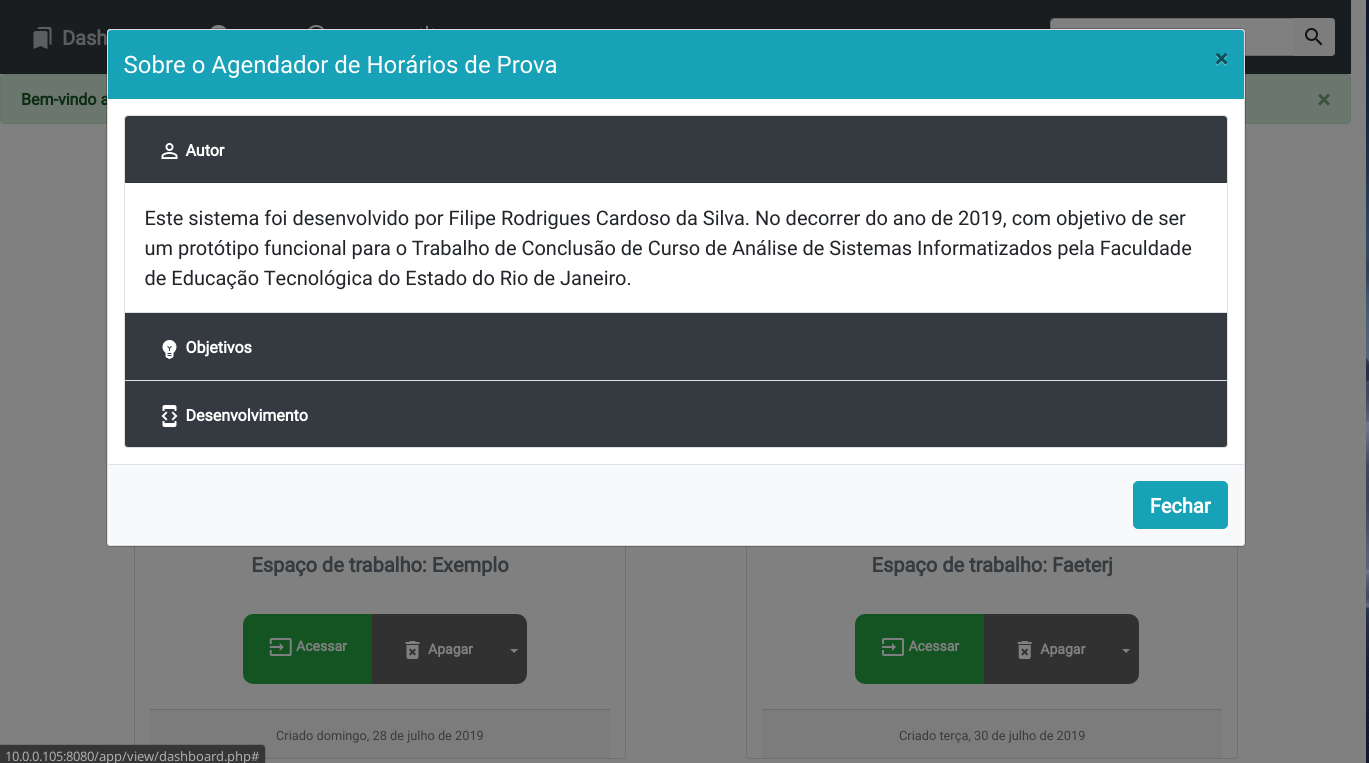
\includegraphics[width=0.8\textwidth]{TCC/imagens/sistema/04.png}
     \caption{Tela Sobre o Sistema}
     \label{tela-sobre}
\end{figure}

Em sequencia temos a opção \textbf{Contato}, que permite o envio de um \textit{e-mail},  conforme visto na figura \ref{tela-contato}, enviando-o para o desenvolvedor do sistema, para informar de possíveis problemas ou possibilitar o contato por qualquer que seja o motivo.
%% Tela Login
\begin{figure}[H]
     \centering
     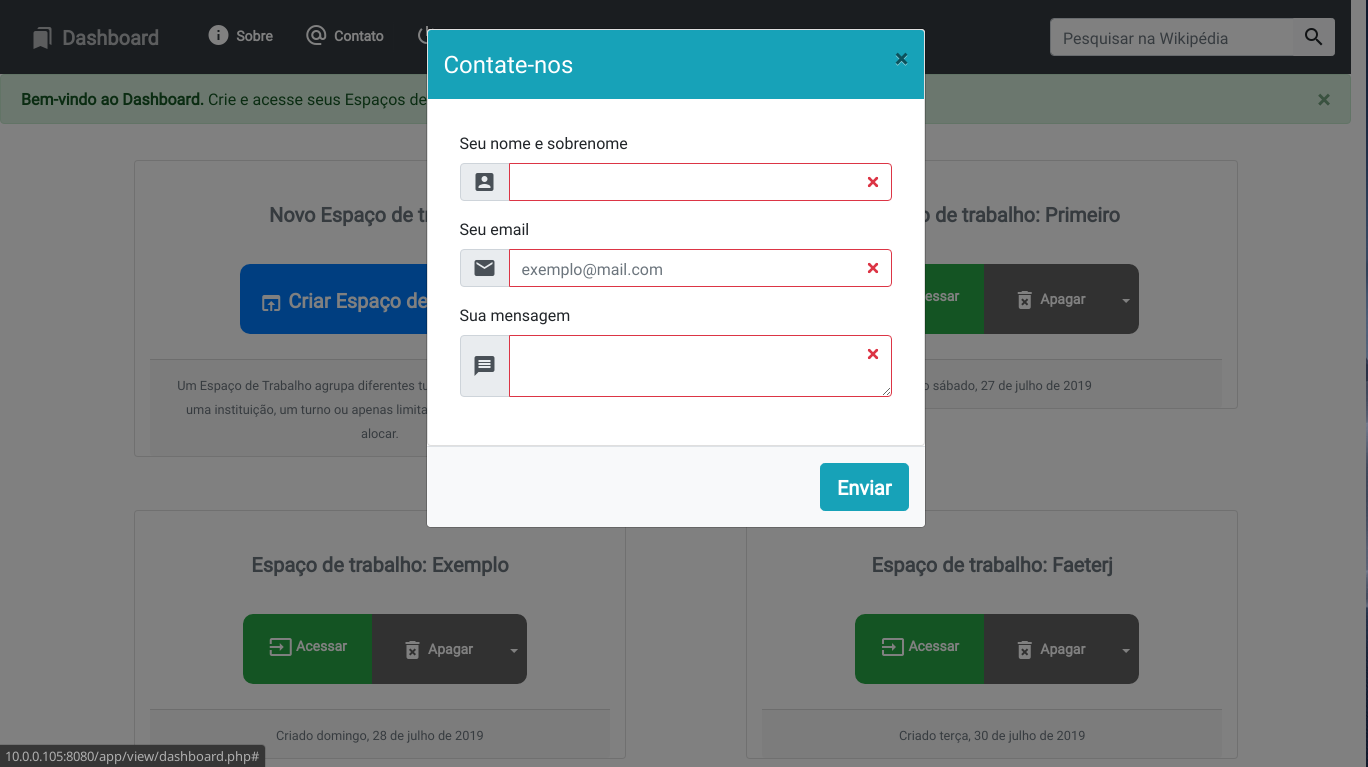
\includegraphics[width=0.8\textwidth]{TCC/imagens/sistema/05.png}
     \caption{Tela de Contato}
     \label{tela-contato}
\end{figure}

No \textbf{\textit{Dashboard}} temos ainda em cada espaço de trabalho as opções de acessar, apagar e um menu flutuante, como mostrada na figura \ref{tela-opcoes-rapidas}, com opções adicionais, facilitando o acesso à algumas funcionalidades do espaço de trabalho como importar e exportar as turmas presentes sem precisar acessar o espaço de trabalho.

%% Tela Login
\begin{figure}[H]
     \centering
     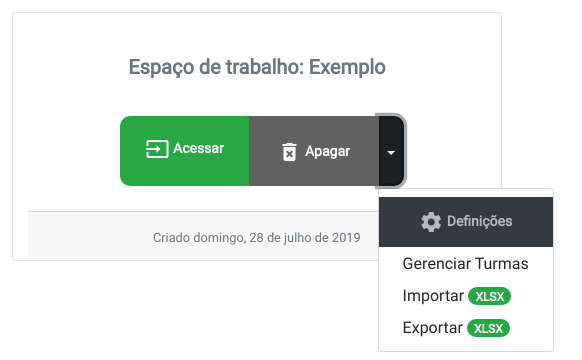
\includegraphics[width=0.8\textwidth]{TCC/imagens/sistema/06.png}
     \caption{Opções Rápidas do Espaço de Trabalho}
     \label{tela-opcoes-rapidas}
\end{figure}

\subsection{Definições do Espaço de Trabalho}

Ao acessar um espaço de trabalho, o usuário é redirecionado para a tela de \textbf{Definições do Espaço de Trabalho}, na qual é possível acessar as opções de configuração daquele espaço.

Dentre as suas opções (figura \ref{tela-definicoes}) temos a opção de criar uma tabela de horários, gerenciar as turmas pertencentes ao espaço de trabalho, adicionar turmas manualmente ou por arquivo (como visto na figura \ref{tela-definicoes-2}) ou exportar as turmas do espaço (figura \ref{tela-definicoes-3}), ainda temos a opção \textbf{Robô}, que demonstra uma explicação do que é o "Robô"\ usado no sistema (figura \ref{tela-robo}).

%% Home 1
\begin{figure}[H]
     \centering
     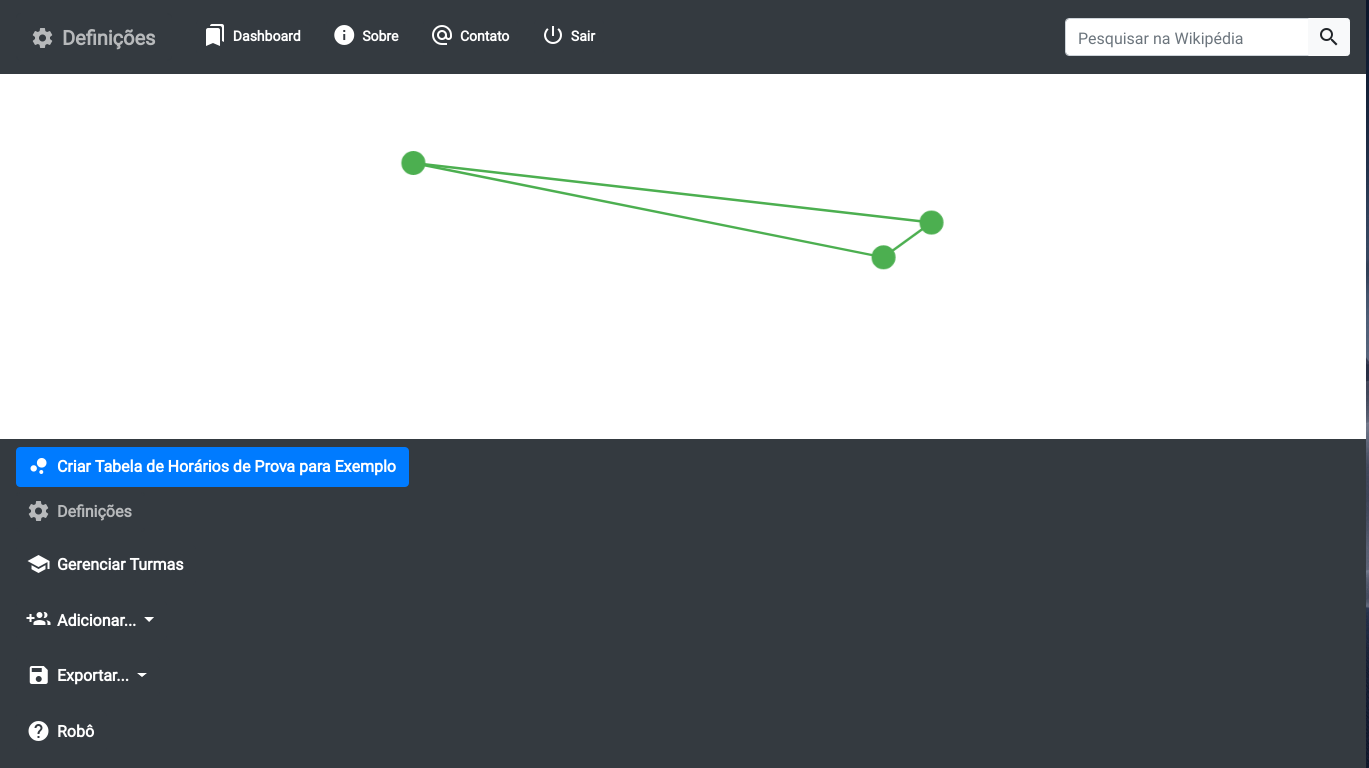
\includegraphics[width=0.8\textwidth]{TCC/imagens/sistema/07.png}
     \caption{Tela de Definições do Espaço de Trabalho}
     \label{tela-definicoes}
\end{figure}

%% Home 2
\begin{figure}[H]
     \centering
     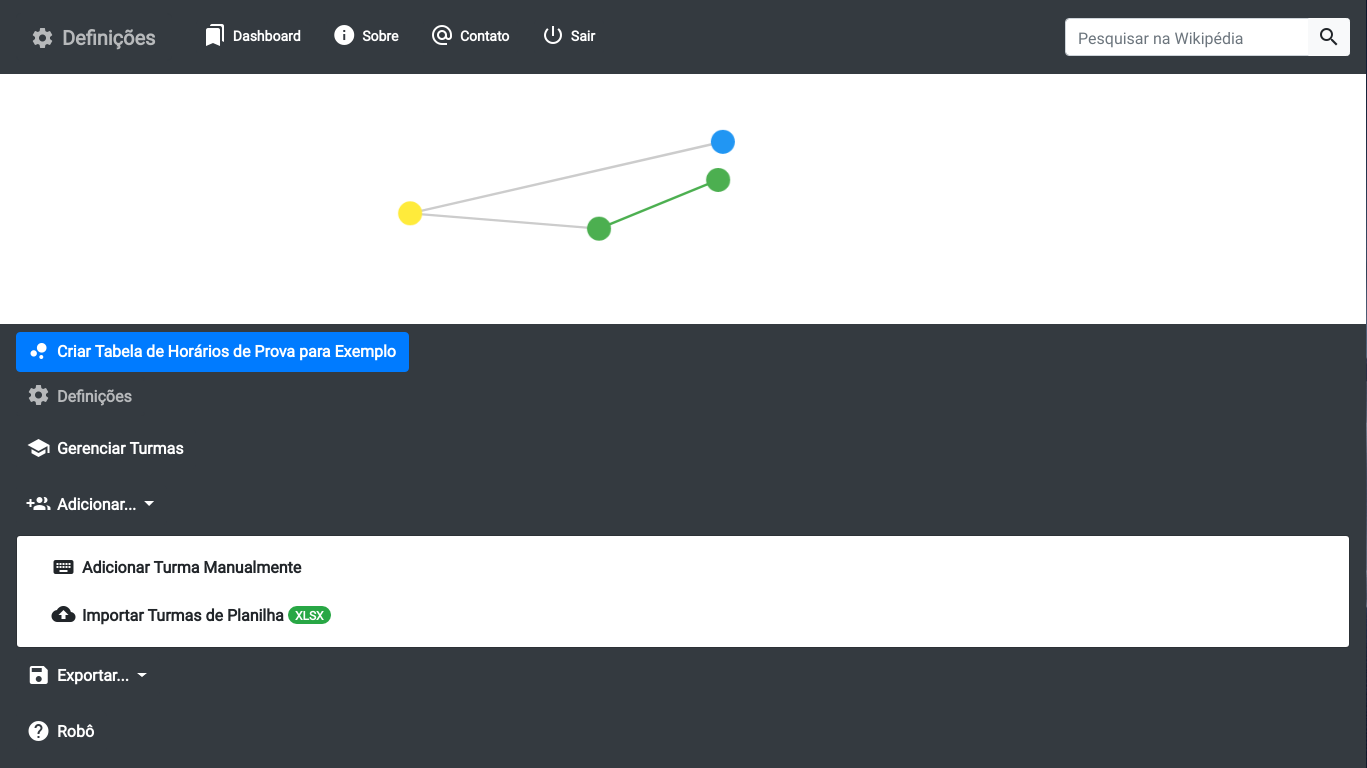
\includegraphics[width=0.8\textwidth]{TCC/imagens/sistema/07b.png}
     \caption{Tela de Definições do Espaço de Trabalho - Caixa de Seleção para Adicionar Dados}
     \label{tela-definicoes-2}
\end{figure}

%% Home 3
\begin{figure}[H]
     \centering
     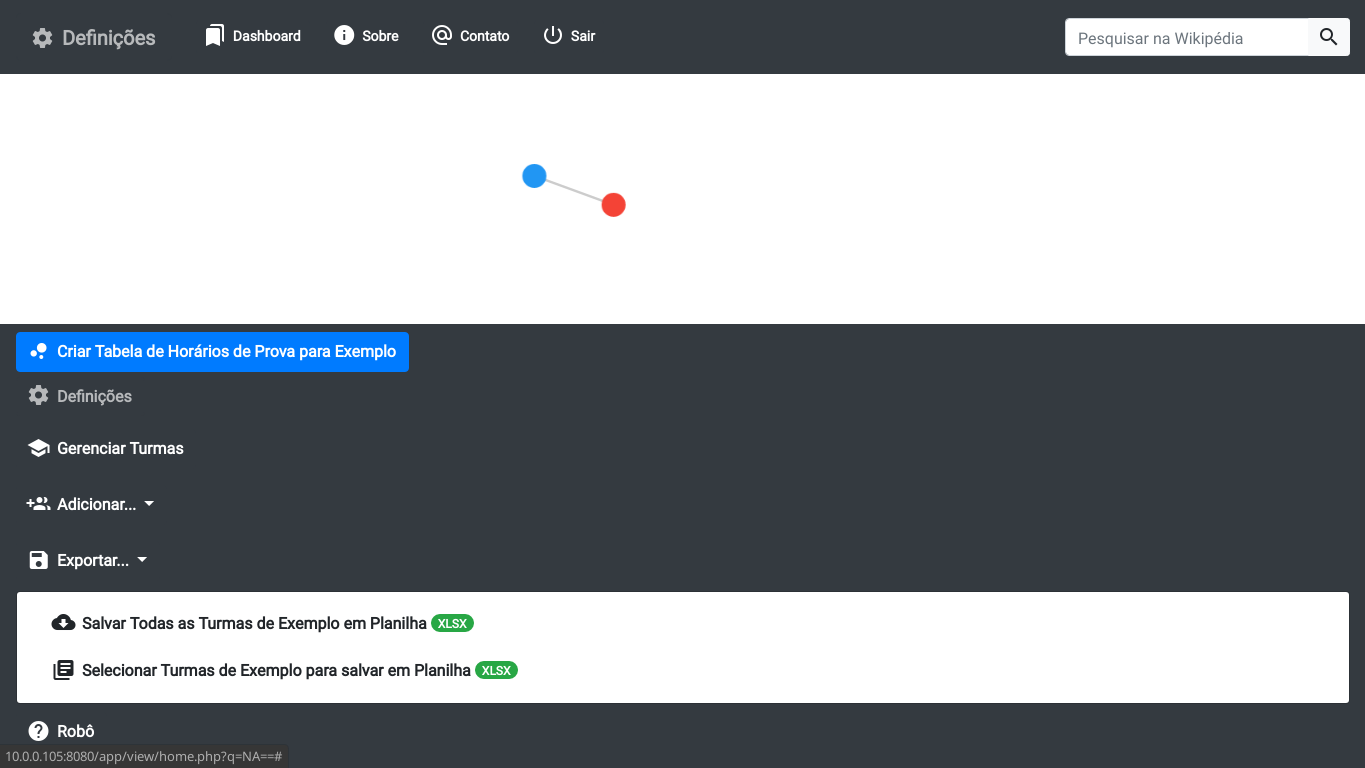
\includegraphics[width=0.8\textwidth]{TCC/imagens/sistema/07c.png}
     \caption{Tela de Definições do Espaço de Trabalho - Caixa de Seleção para Exportar Dados}
     \label{tela-definicoes-3}
\end{figure}

%% Home 4
\begin{figure}[H]
     \centering
     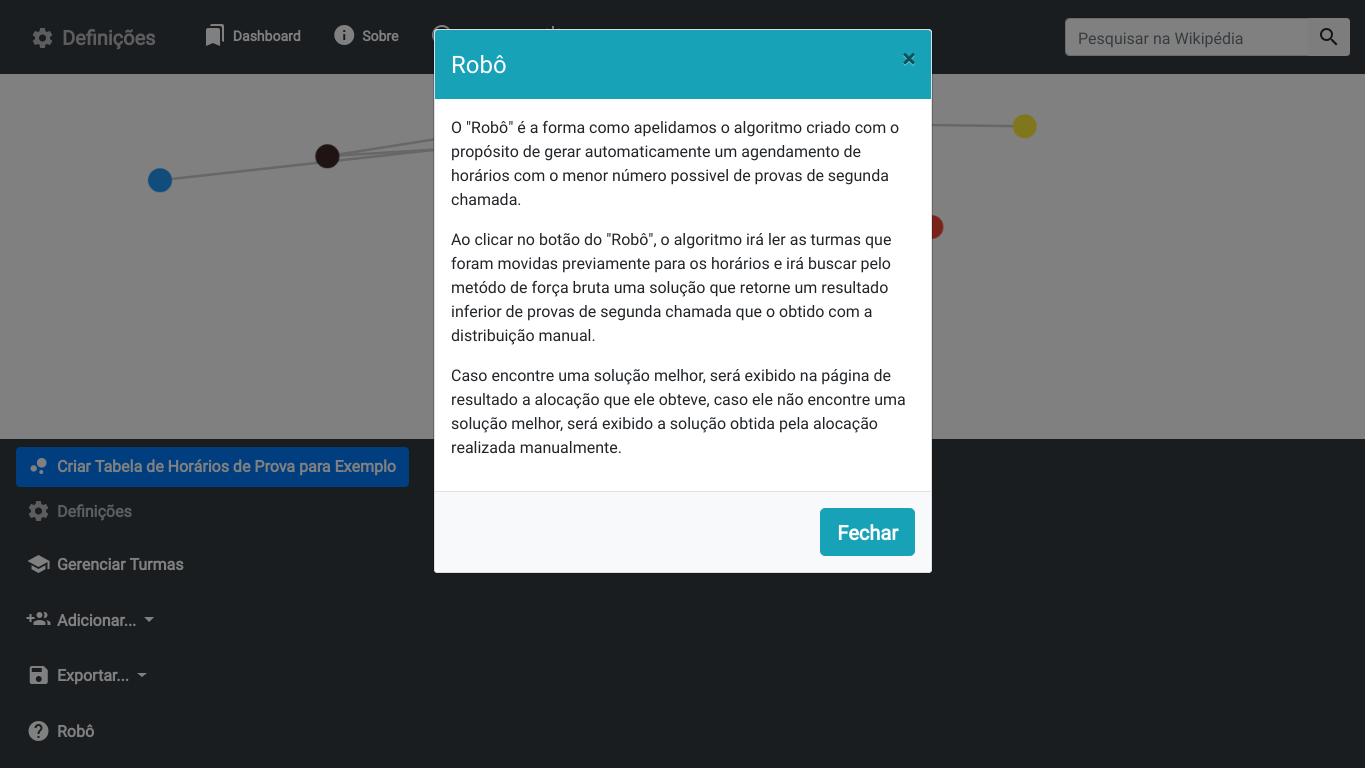
\includegraphics[width=0.8\textwidth]{TCC/imagens/sistema/07d.png}
     \caption{Tela de Explicação da Solução através do uso do Robô}
     \label{tela-robo}
\end{figure}

\subsection{Gerenciar Turmas}

Ao acessar a opção de \textbf{Gerenciar Turmas}, o usuário é direcionado para a página em que visualizará as turmas que estão presentes naquele espaço de trabalho (figura \ref{tela-gerenciador}). Nesta página o usuário poderá \textbf{adicionar uma turma}, e caso já tenha adicionado turmas, terá as opções de visualizar, editar e apagar as turmas e seus alunos.

Quando selecionada a opção de \textbf{visualizar turma}, o usuário tem acesso a uma listagem de alunos que pertencem aquela turma (figura \ref{tela-visu-1}), a opção de retornar a tela de gerenciamento de turmas, e a de edição da turma (figura \ref{tela-visu-2}).
%% Gerenciar turmas
\begin{figure}[H]
     \centering
     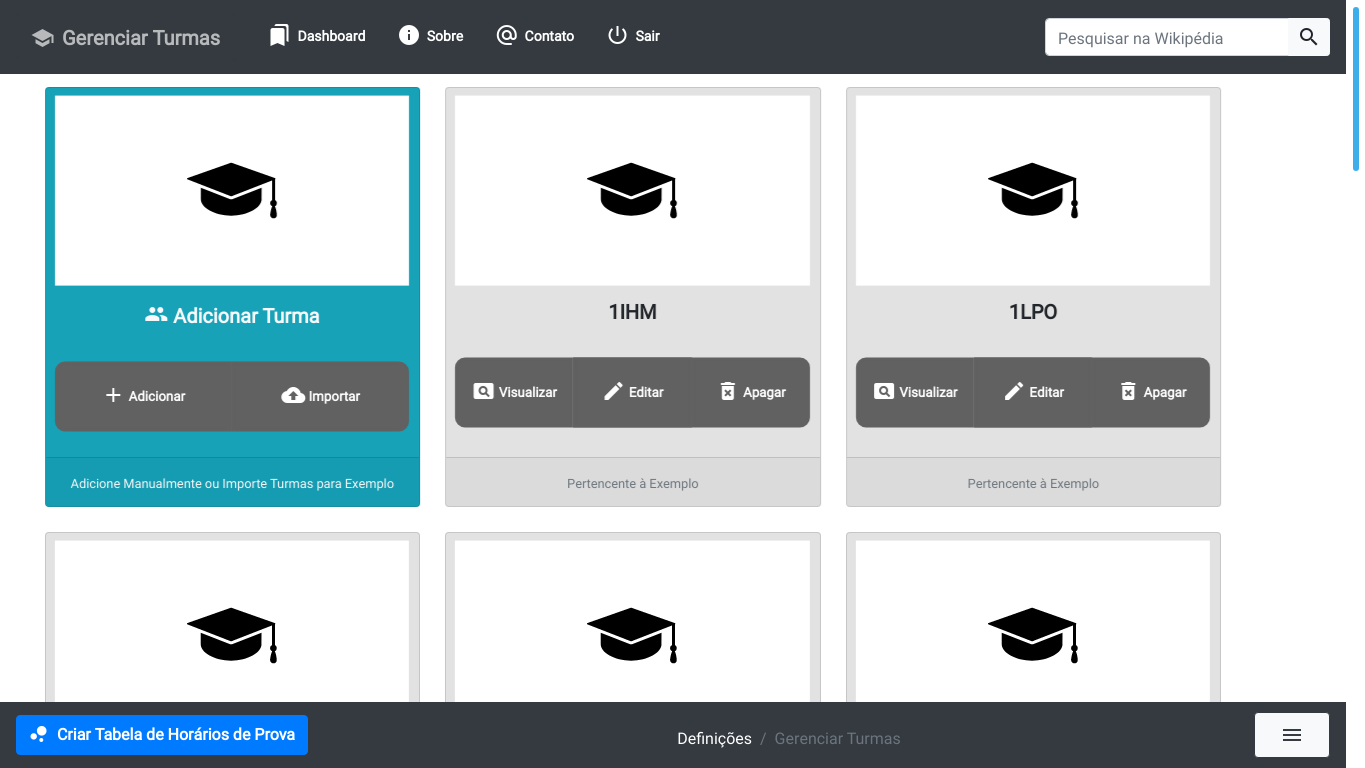
\includegraphics[width=0.8\textwidth]{TCC/imagens/sistema/08.png}
     \caption{Tela de Gerenciamento de Turmas}
     \label{tela-gerenciador}
\end{figure}

%% Visualizar alunos da turma 1
\begin{figure}[H]
     \centering
     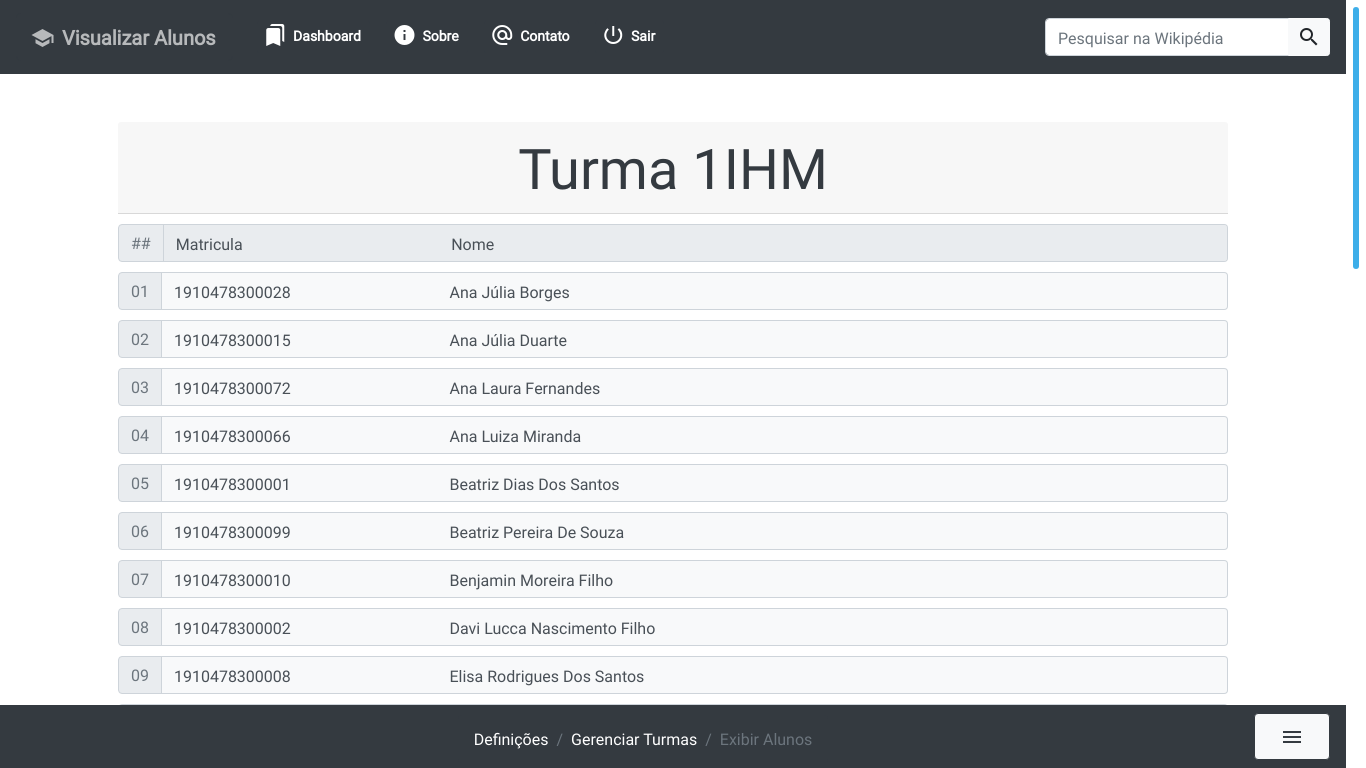
\includegraphics[width=0.8\textwidth]{TCC/imagens/sistema/09.png}
     \caption{Tela de Visualização da Turma}
     \label{tela-visu-1}
\end{figure}

%% Visualizar alunos da turma 2
\begin{figure}[H]
     \centering
     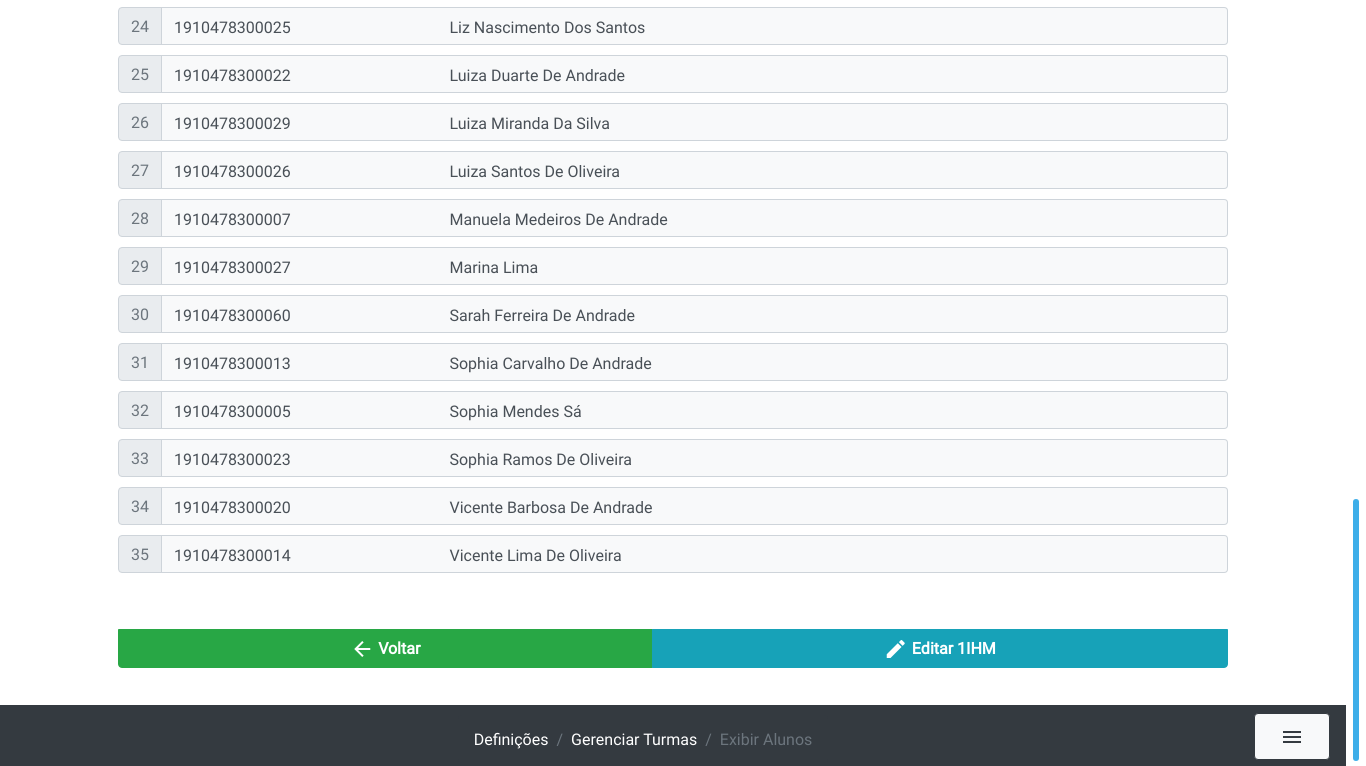
\includegraphics[width=0.8\textwidth]{TCC/imagens/sistema/09b.png}
     \caption{Tela de Visualização da Turma -- Cont.}
     \label{tela-visu-2}
\end{figure}

Para se \textbf{editar uma turma}, o usuário será direcionado para a página de edição (figura \ref{tela-edit-1}), onde poderá modificar a matrícula ou nome de um aluno em especifico, remove-lo da turma ou adicionar um novo aluno na turma (figura \ref{tela-edit-2}).


%% Editar alunos da turma 1
\begin{figure}[H]
     \centering
     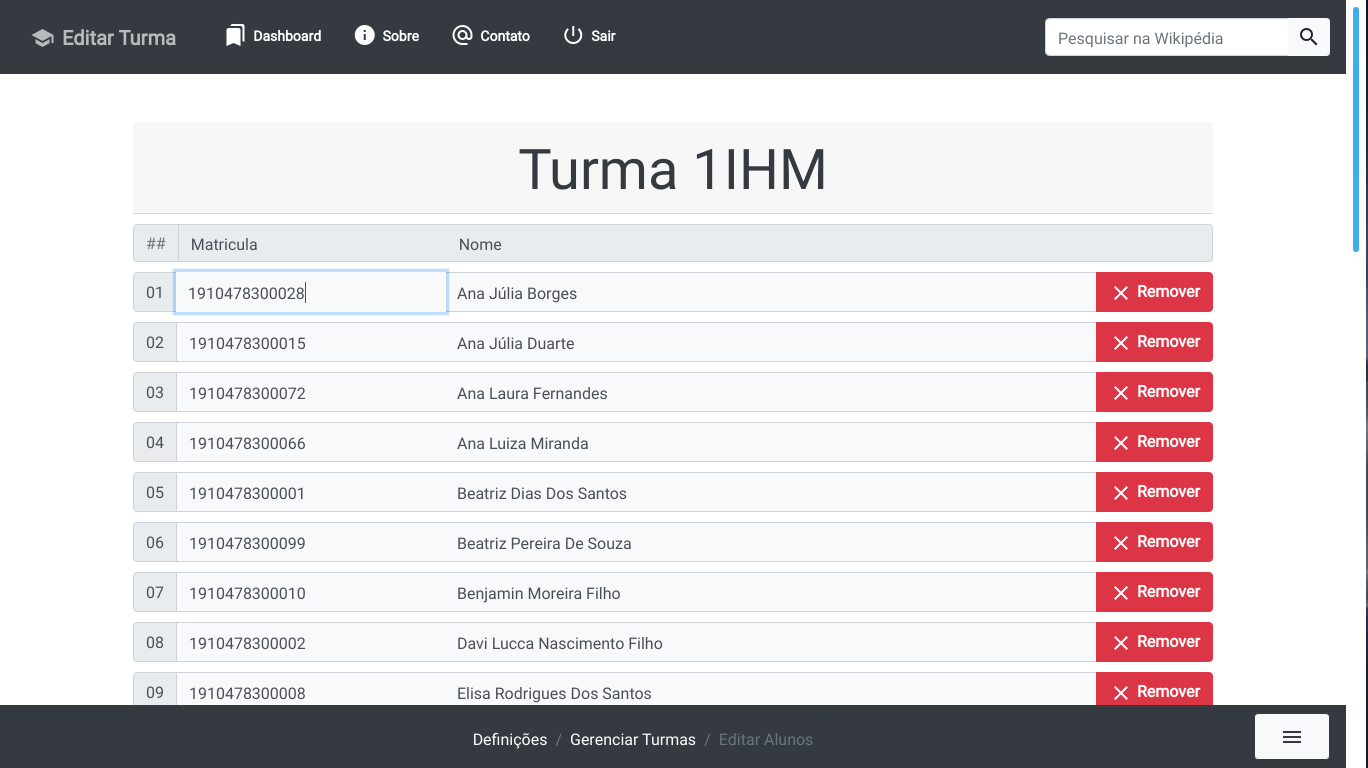
\includegraphics[width=0.8\textwidth]{TCC/imagens/sistema/10a.png}
     \caption{Tela de Edição de Turmas}
     \label{tela-edit-1}
\end{figure}

%% Editar alunos da turma 2
\begin{figure}[H]
     \centering
     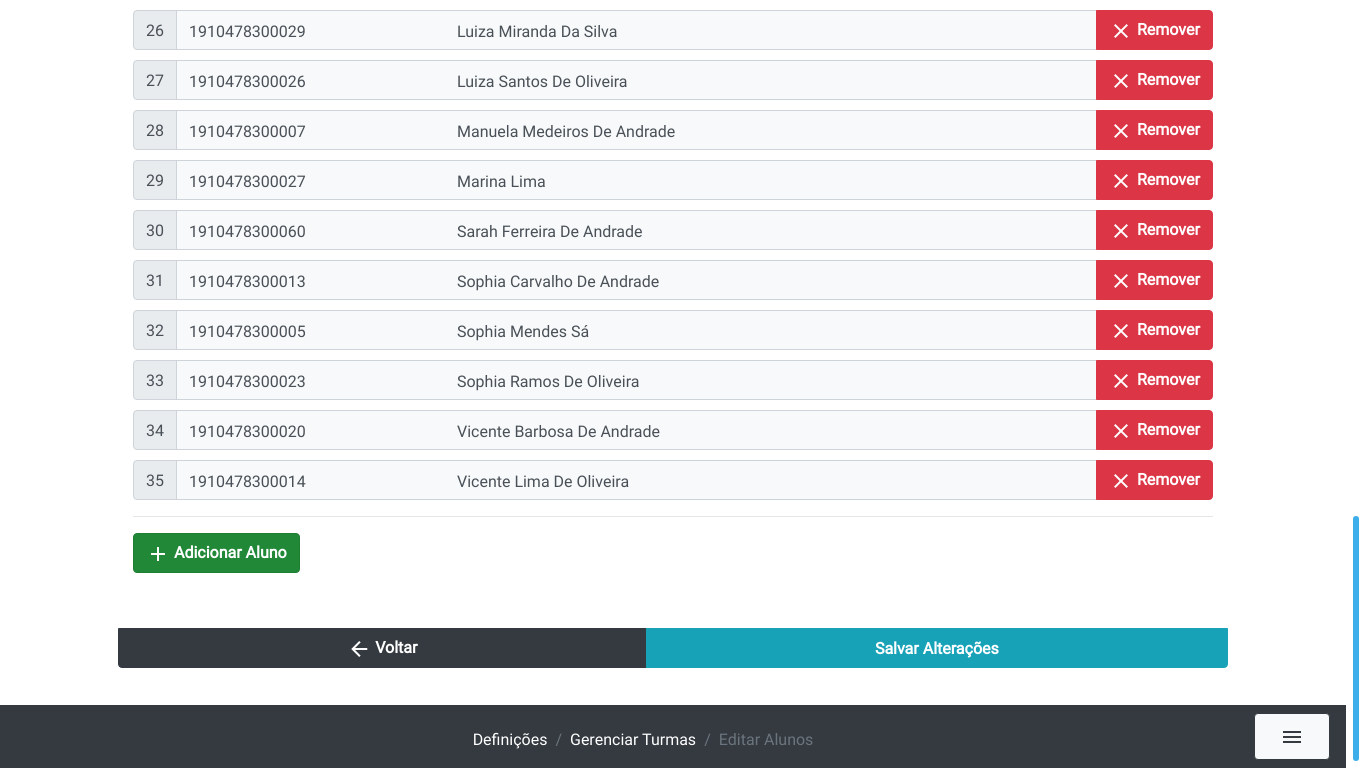
\includegraphics[width=0.8\textwidth]{TCC/imagens/sistema/10b.png}
     \caption{Tela de Edição de Turmas -- Cont.}
     \label{tela-edit-2}
\end{figure}

Para se \textbf{apagar uma turma}, uma mensagem irá informar que, ao apagar a turma ela não poderá ser recuperada posteriormente (figura \ref{tela-delete}).

%% Apagar turma
\begin{figure}[H]
     \centering
     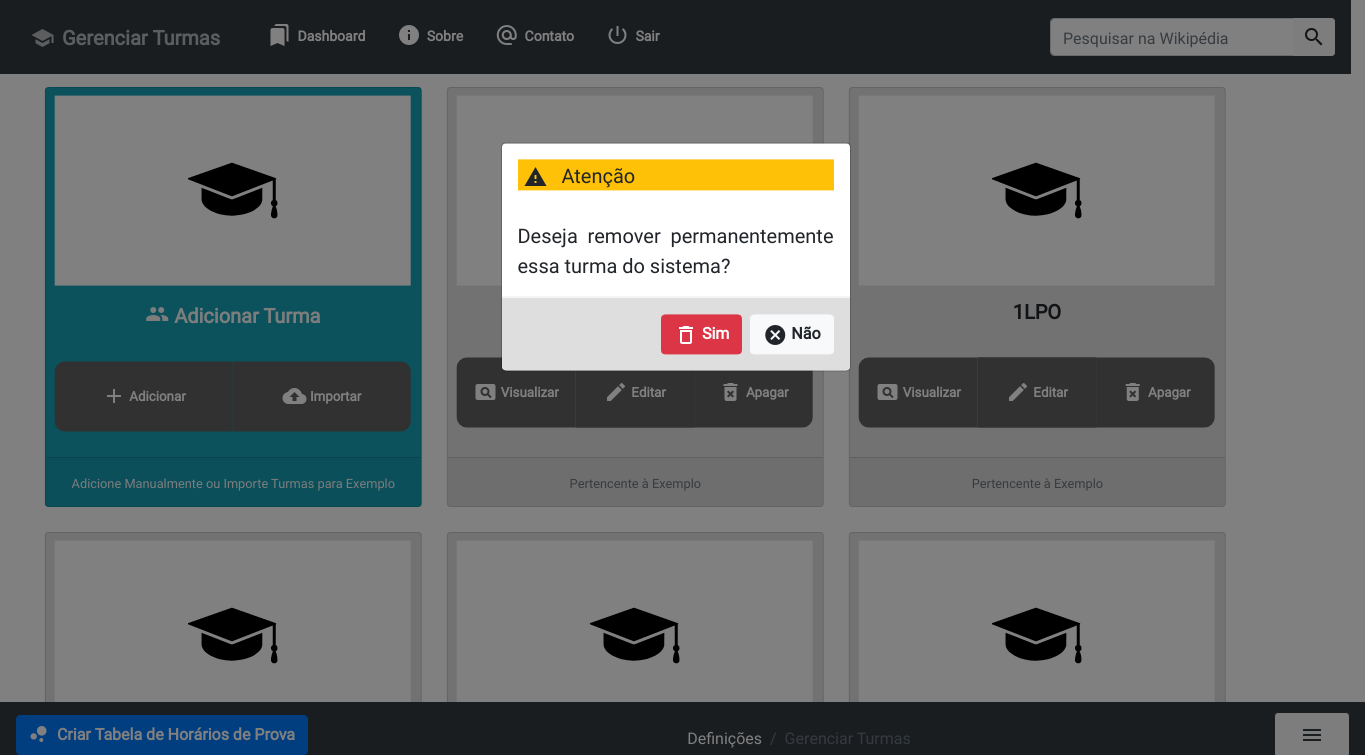
\includegraphics[width=0.8\textwidth]{TCC/imagens/sistema/11.png}
     \caption{Notificação ao Apagar Turma}
     \label{tela-delete}
\end{figure}

Para criar uma nova turma o usuário deverá \textbf{Adicionar Turma} na tela de \textbf{Gerenciamento de Turmas} (conforme na figura \ref{tela-gerenciador}), e para incluir a nova turma deverá informar o nome dessa turma (figura \ref{tela-create}), e opcionalmente deverá informar os alunos que a compõe, informando a matrícula e o nome completo do aluno (figura \ref{tela-create-2}).
%% Criar turma 1
\begin{figure}[H]
     \centering
     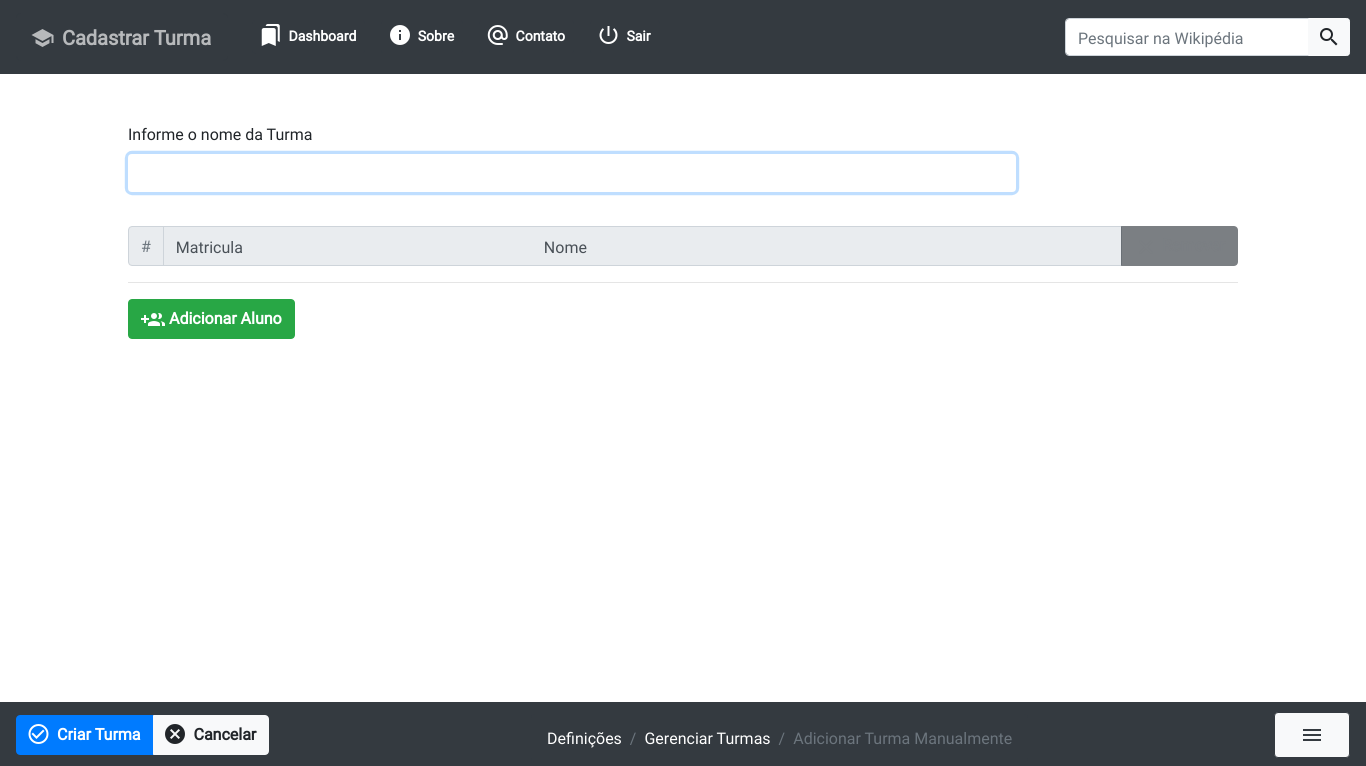
\includegraphics[width=0.8\textwidth]{TCC/imagens/sistema/14.png}
     \caption{Tela de Criação de Nova Turma}
     \label{tela-create}
\end{figure}

%% Criar turma 2
\begin{figure}[H]
     \centering
     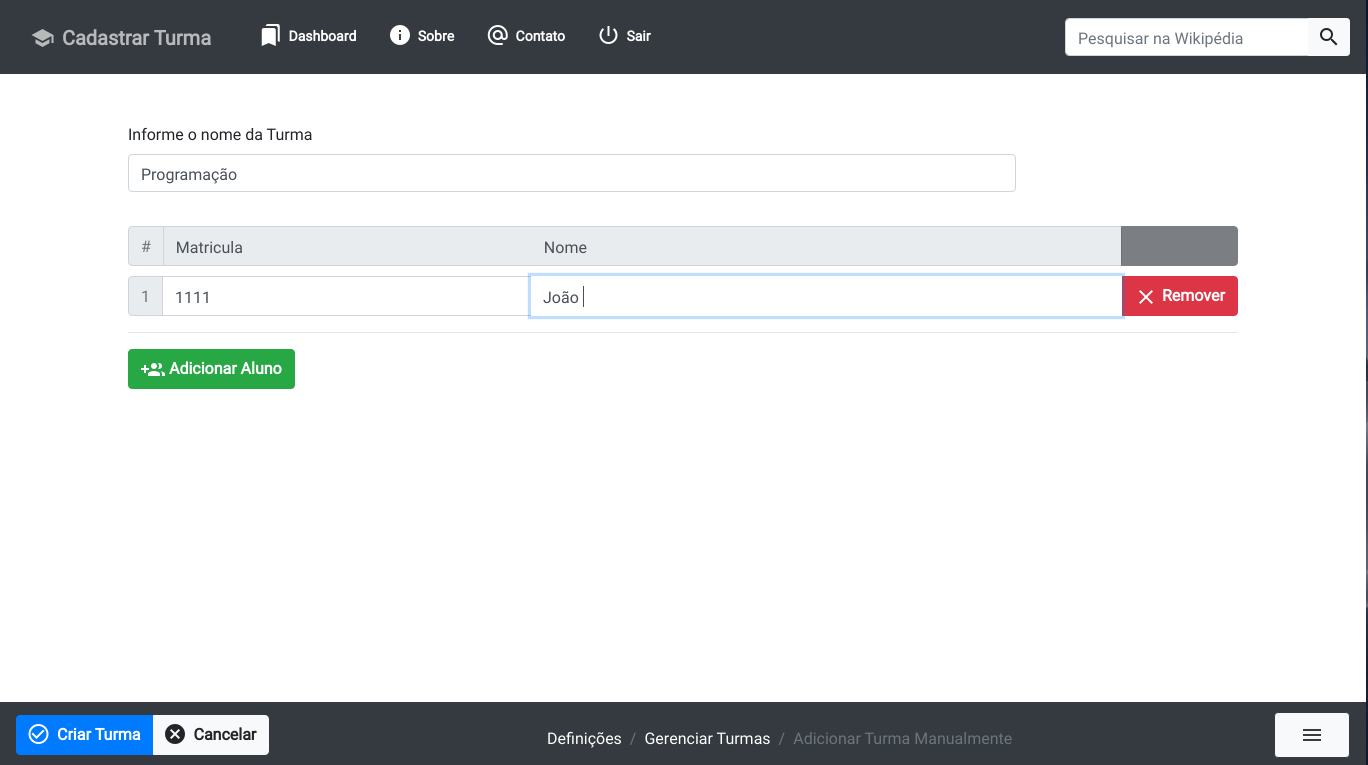
\includegraphics[width=0.8\textwidth]{TCC/imagens/sistema/14a.png}
     \caption{Tela de Criação de Nova Turma -- Cont.}
     \label{tela-create-2}
\end{figure}

Outra opção na página de Gerenciamento de turmas é a \textbf{inclusão de turmas por importação de um arquivo XSLX} (planilha \textit{MS Excel}), que deve estar formatada de acordo com o padrão do sistema e assim só será necessário realizar o \textit{update} do arquivo clicando em enviar e as turmas serão importadas para o espaço de trabalho (figura \ref{tela-import}).

%% Importar turmas de planilha
\begin{figure}[H]
     \centering
     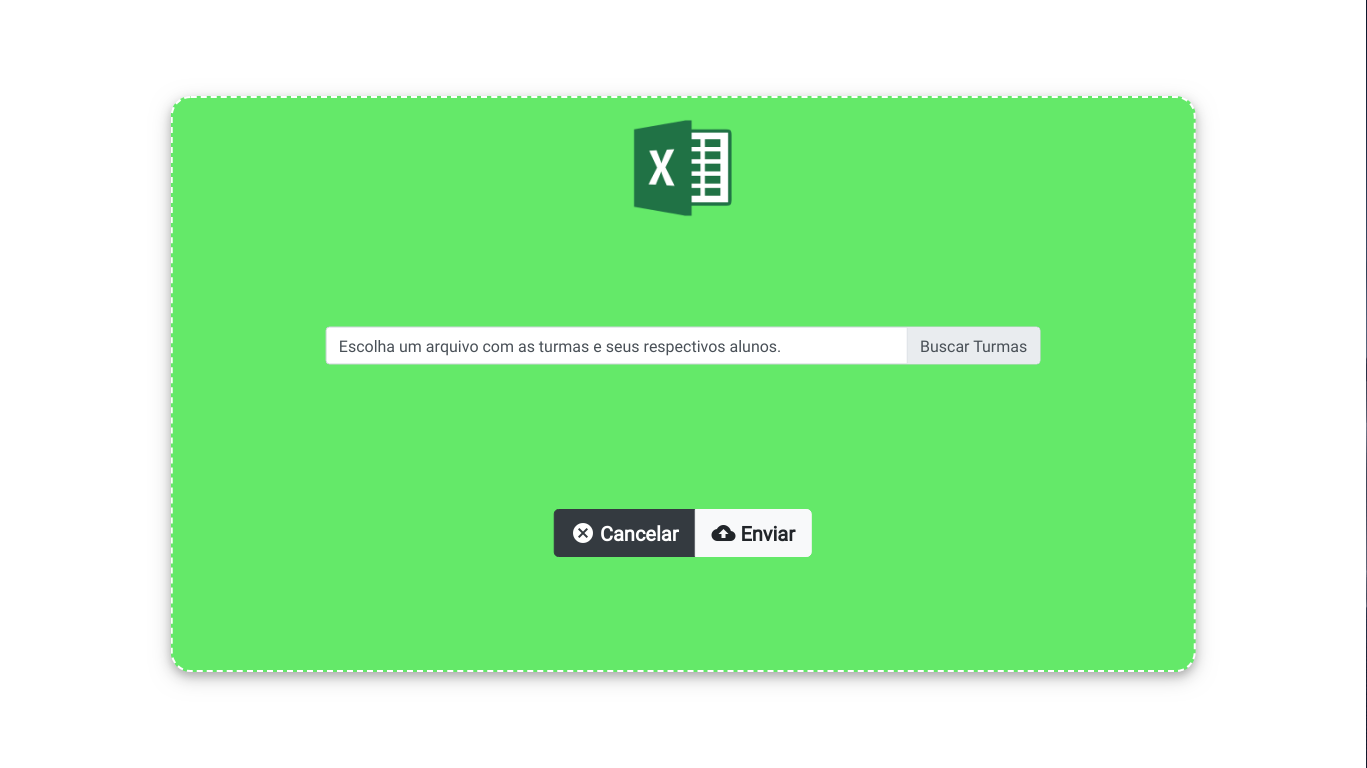
\includegraphics[width=0.8\textwidth]{TCC/imagens/sistema/15.png}
     \caption{Tela de Importação de Turmas por Arquivo}
     \label{tela-import}
\end{figure}

\subsection{Alocar Turmas em Horários de Prova}

A tela onde iremos \textbf{alocar as turmas nos horários de prova} é a principal página do sistema, pois é aqui que criaremos as tabelas de horários de prova (figura \ref{tela-aloc-2h}). Devemos informar nessa página a quantidade de horários que dispomos para realizar as provas (na figura \ref{tela-aloc-3h} foi definido que existem três horários disponíveis para realizar a prova).
%% Alocar 1
\begin{figure}[H]
     \centering
     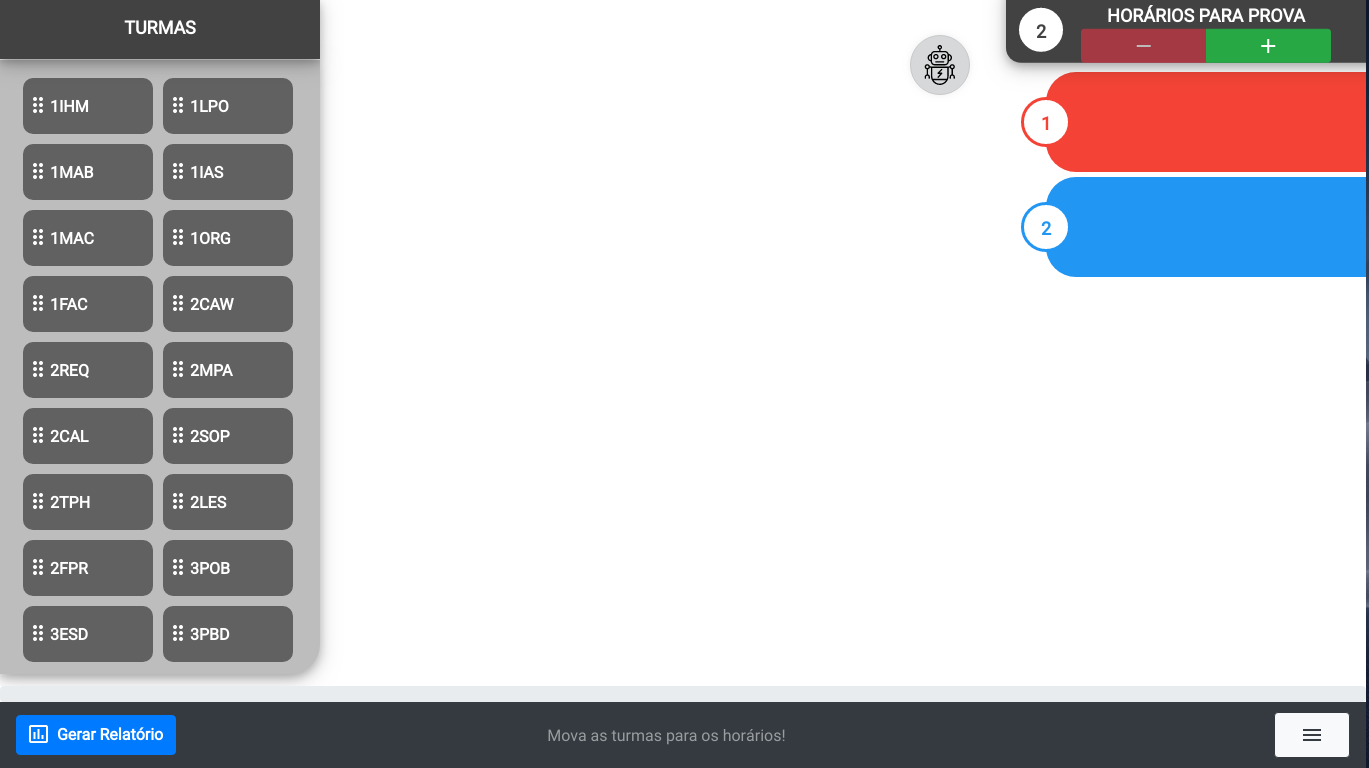
\includegraphics[width=0.8\textwidth]{TCC/imagens/sistema/12a.png}
     \caption{Tela de Alocar Turmas em 2 Horários}
     \label{tela-aloc-2h}
\end{figure}

%% Alocar 2
\begin{figure}[H]
     \centering
     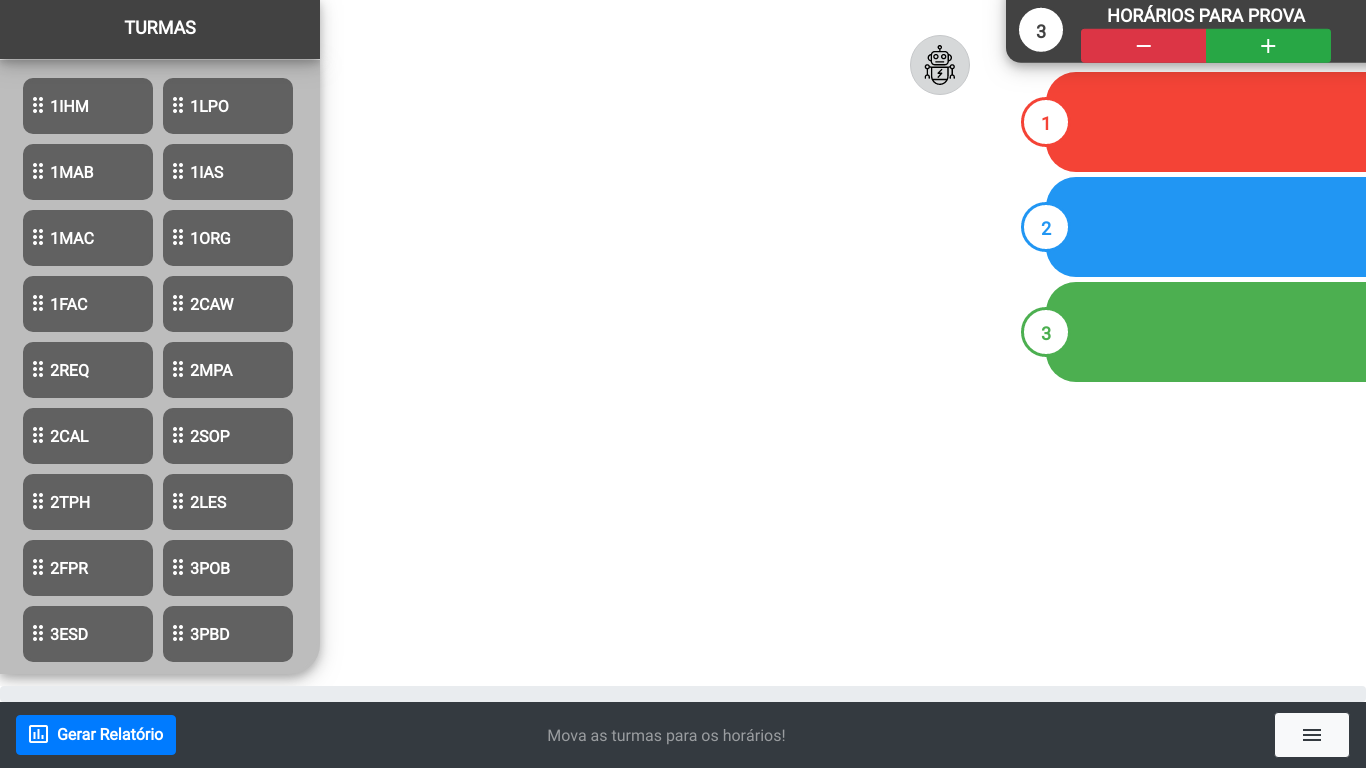
\includegraphics[width=0.8\textwidth]{TCC/imagens/sistema/12b.png}
     \caption{Tela de Alocar Turmas em 3 Horários}
     \label{tela-aloc-3h}
\end{figure}

Na barra situada na parte de baixo na página temos o menu secundário (figura \ref{tela-aloc-menu}), que apresenta as opções referentes ao espaço de trabalho e as turmas, assim como opções já apresentadas.
%% Alocar 1
\begin{figure}[H]
     \centering
     \includegraphics[width=0.8\textwidth]{TCC/imagens/sistema/12b-2.png}
     \caption{Tela de Alocar Turmas em 3 Horários -- Menu}
     \label{tela-aloc-menu}
\end{figure}


%% ===========================================================
%% ===========   EXEMPLO DE ALOCAÇÃO DE TURMAS ===============

    \begin{table}[h]
        \centering
        \caption{Exemplos de alocações e seus resultados}
        \vspace{0.5cm}
        \renewcommand\arraystretch{1.5}
        \begin{tabular}{c|c|c|c|c}
         
            \textbf{Figura} & \textbf{Moveu as Turmas} & \textbf{Para os Horários}  & \textbf{Conflitos} & \textbf{Taxa de Conflitos}\\ % Note a separação de col. e a quebra de linhas
            \hline                               % para uma linha horizontal
            \ref{tela-aloc-ex1} &   1HM  &   1  &    0   & 0\% \\
            \ref{tela-aloc-ex2} &   1IAS  &   2  &    0   & 0\% \\
            \ref{tela-aloc-ex3} &   1MAB  &   3  &    0   & 0\% \\
            \ref{tela-aloc-ex4} &  1LPO e 1IAS   &   2 e 1  &    8   & 15\% \\ 
            \ref{tela-aloc-ex5} &  1MAC e 1ORG   &  2 e 3   &    26   & 19\% \\ 
            \ref{tela-aloc-ex6} &   TODAS  &   1  &    140   & 100\% \\ 
            \ref{tela-aloc-ex7} &   1LPO, 1MAB, 1IAS  &   2  &    57   & 41\%
            % não é preciso quebrar a última linha
            \\
            \hline
        \end{tabular}
        \label{tabela-exemplo}
    \end{table}

Para se alocar uma turma em um horário basta clicar na turma, manter pressionado e arrastar até o \textbf{\textit{slot}} de horário desejado. Na tabela \ref{tabela-exemplo} temos descrita uma sequência de movimentações para exemplificar o funcionamento dessa tela. 

Os conflitos são correspondentes ao número de provas de segunda chamada, necessárias para a realização daquela tabela de horários de prova. 

A taxa de conflitos é obtida através do maior número de conflito possível para as turmas selecionadas, divido pela quantidade de conflitos da solução atual multiplicado por 100.






%% ===========================================================

%% Alocar 2
\begin{figure}[H]
     \centering
     \includegraphics[width=0.8\textwidth]{TCC/imagens/sistema/12c.png}
     \caption{Tela de Alocar Turmas -- Exemplo 1}
     \label{tela-aloc-ex1}
\end{figure}

%% Alocar 1
\begin{figure}[H]
     \centering
     \includegraphics[width=0.8\textwidth]{TCC/imagens/sistema/12d.png}
     \caption{Tela de Alocar Turmas -- Exemplo 2}
     \label{tela-aloc-ex2}
\end{figure}

%% Alocar 2
\begin{figure}[H]
     \centering
     \includegraphics[width=0.8\textwidth]{TCC/imagens/sistema/12e.png}
     \caption{Tela de Alocar Turmas -- Exemplo 3}
     \label{tela-aloc-ex3}
\end{figure}

%% Alocar 1
\begin{figure}[H]
     \centering
     \includegraphics[width=0.8\textwidth]{TCC/imagens/sistema/12f.png}
     \caption{Tela de Alocar Turmas -- Exemplo 4}
     \label{tela-aloc-ex4}
\end{figure}

%% Alocar 2
\begin{figure}[H]
     \centering
     \includegraphics[width=0.8\textwidth]{TCC/imagens/sistema/12g.png}
     \caption{Tela de Alocar Turmas -- Exemplo 5}
     \label{tela-aloc-ex5}
\end{figure}



%% Alocar 2
\begin{figure}[H]
     \centering
     \includegraphics[width=0.8\textwidth]{TCC/imagens/sistema/12h.png}
     \caption{Tela de Alocar Turmas -- Exemplo 6}
     \label{tela-aloc-ex6}
\end{figure}

%% Alocar 2
\begin{figure}[H]
     \centering
     \includegraphics[width=0.8\textwidth]{TCC/imagens/sistema/12i.png}
     \caption{Tela de Alocar Turmas -- Exemplo 7}
     \label{tela-aloc-ex7}
\end{figure}



 





\subsection{Gerar Relatório da Alocação}
%% ===========================================================
%% ===========   EXEMPLO DE GERAÇÃO DE RESULTADO =============


Agora vamos usar a tabela de horários de prova mostrada na figura \ref{tela-grade1} como a grade de horários que desejamos utilizar, dessa forma podemos clicar no botão \textbf{Gerar Relatório} para concluir a alocação das turmas e visualizar o resultado de forma detalhada como nas figuras \ref{tela-grade2} e \ref{tela-grade3}.

Na figura \ref{tela-grade4} percebemos que em caso de clicarmos na linha da imagem (aresta do Grafo) será exibido os alunos que pertencem as duas turmas que a linha conecta. Já na figura \ref{tela-grade5} vemos que ao clicar na turma (no vértice do Grafo) temos a lista com todos os alunos pertencentes aquela turma.

%% ===========================================================
%% Alocando Turmas 1
\begin{figure}[H]
     \centering
     \includegraphics[width=0.8\textwidth]{TCC/imagens/sistema/13a.png}
     \caption{Gerando uma Grade de Prova -- pt. 1}
     \label{tela-grade1}
\end{figure}

%% Alocando Turmas 2
\begin{figure}[H]
     \centering
     \includegraphics[width=0.8\textwidth]{TCC/imagens/sistema/13b-1.png}
     \caption{Gerando uma Grade de Prova -- pt. 2}
     \label{tela-grade2}
\end{figure}



%% Alocando Turmas 3
\begin{figure}[H]
     \centering
     \includegraphics[width=0.8\textwidth]{TCC/imagens/sistema/13b-2.png}
     \caption{Gerando uma Grade de Prova -- pt. 3}
     \label{tela-grade3}
\end{figure}

%% Alocando Turmas 4
\begin{figure}[H]
     \centering
     \includegraphics[width=0.8\textwidth]{TCC/imagens/sistema/13b-3.png}
     \caption{Gerando uma Grade de Prova -- pt. 4}
     \label{tela-grade4}
\end{figure}

%% Alocando Turmas 5
\begin{figure}[H]
     \centering
     \includegraphics[width=0.8\textwidth]{TCC/imagens/sistema/13b-4.png}
     \caption{Gerando uma Grade de Prova -- pt. 5}
     \label{tela-grade5}
\end{figure}

Ao final da página de relatório temos uma opção descrita como "Deseja tentar encontrar um resultado melhor usando nosso robô?"\ (figura \ref{tela-grade6}), essa opção irá utilizar o algoritmo criado para o sistema para buscar a melhor distribuição de turmas nos horários, isto é a alocação que vai gerar o menor número de provas de segunda chamada por conflitos de horário. 


%% Alocando Turmas 6
\begin{figure}[H]
     \centering
     \includegraphics[width=0.8\textwidth]{TCC/imagens/sistema/13b-5.png}
     \caption{Gerando uma Grade de Prova -- pt. 6}
     \label{tela-grade6}
\end{figure}

Caso o usuário opte por essa opção ele será redirecionado para uma nova página de \textbf{relatório} (figura \ref{tela-grade7}). 

Vale dizer que caso o usuário clicasse no \textbf{botão do "Robô"}\ na página de\textbf{ criação de tabela de horário} (figuras \ref{tela-aloc-2h} e \ref{tela-aloc-3h} ele seria direcionado para esse mesmo relatório.

Vemos na figura \ref{tela-grade7} que além de apresentar a quantidade de provas necessárias para realização das provas, esse relatório também irá apresentar a quantidade de provas necessárias na solução manual, que foi gerada anteriormente, e o quanto o "Robô"\ conseguiu melhorar o resultado manual. 

Além das diferenças já citadas, a página vai apresentar as mesmas informações quanto aos horários em que as turmas foram alocadas, e uma figura interativa (de um Grafo) que representa a relação entre as turmas, contanto não haverá mais a opção de tentar uma solução melhor com o "Robô"\ já que essa se trata da melhor solução possível (figura \ref{tela-grade8}).


%% Alocando Turmas 5
\begin{figure}[H]
     \centering
     \includegraphics[width=0.8\textwidth]{TCC/imagens/sistema/13c-1.png}
     \caption{Gerando uma Grade de Prova -- pt. 7}
     \label{tela-grade7}
\end{figure}

%% Alocando Turmas 5
\begin{figure}[H]
     \centering
     \includegraphics[width=0.8\textwidth]{TCC/imagens/sistema/13c-2.png}
     \caption{Gerando uma Grade de Prova -- pt. 8}
     \label{tela-grade8}
\end{figure}



\subsection{Imprimir Relatório}

Na base da tela de relatório temos o menu secundário com algumas opções semelhantes as que já foram apresentadas (figura \ref{tela-grade9}), e além dessas existe a opção de \textbf{Imprimir Relatório}, a qual possibilita gerar um arquivo para impressão ou para \textit{download} (figura \ref{tela-relatorio}).

%% Alocando Turmas 5
\begin{figure}[H]
     \centering
     \includegraphics[width=0.8\textwidth]{TCC/imagens/sistema/13c-3.png}
     \caption{Gerando uma Grade de Prova -- pt. 9}
     \label{tela-grade9}
\end{figure}
%% Tela Relatório em PDF
\begin{figure}[H]
     \centering
     \includegraphics[width=0.8\textwidth]{TCC/imagens/sistema/13d-1.png}
     \caption{Gerando Relatório}
     \label{tela-relatorio}
\end{figure}


\includepdf[pages=1,pagecommand=\chapter{Relatório}\label{cap:resultado}]{arquivos/anexo-b.pdf}

\end{anexosenv}

\includepdf[pages=2-]{arquivos/anexo-b.pdf}
   
    % -------------------------------------------------------------
	% Índice Remissivo
	% -------------------------------------------------------------
 	 \phantompart								%
	\printindex									%
 	
\end{document}

% --------------------------------------------------------------------
%
%							FIM DO DOCUMENTO
%
% --------------------------------------------------------------------